\documentclass{standalone} % Utilise la classe standalone pour compiler uniquement le TikZ
%\include{pakage_tikz}
\usepackage{tikz}          % Charge le package TikZ
\usepackage{xcolor}        % Gestion avancée des couleurs
\usepackage{amsmath}       % Gestion des formules mathématiques
\usetikzlibrary{arrows.meta} % Pour gérer les flèches avec des formes spécifiées comme "triangle"
\usetikzlibrary {decorations.pathmorphing}
\usepackage{pgfplots}
\pgfplotsset{compat=1.18}
\usepackage[active,tightpage]{preview}
\PreviewEnvironment{tikzpicture}
\usetikzlibrary{arrows.meta}
\usetikzlibrary {arrows.meta,bending,positioning}
\usetikzlibrary {datavisualization.formats.functions}
%PREAMBULE pour schÃéma
\usepackage{pgfplots}
\usepackage{tikz}
\usepackage[european resistor, european voltage, european current]{circuitikz}
\usetikzlibrary{arrows,shapes,positioning}
\usetikzlibrary{decorations.markings,decorations.pathmorphing,
decorations.pathreplacing}
\usetikzlibrary{calc,patterns,shapes.geometric}
\usepackage{anyfontsize}
\usepackage{bm}

\usetikzlibrary {fadings,patterns}
\usetikzlibrary{hobby} % <-- indispensable pour use Hobby shortcut

\setlength\PreviewBorder{5pt}
%\usepgfplotslibrary{external}
%\tikzexternalize

%% Automatiser cela : une solution plus élégante  nouvelle page, tu peux utiliser la commande \newpage juste avant chaque \begin{tikzpicture}
%\let\oldtikzpicture\tikzpicture
%\let\endoldtikzpicture\endtikzpicture
%\renewenvironment{tikzpicture}{\newpage\oldtikzpicture}{\endoldtikzpicture}
%\usepackage{etoolbox} % dans le préambule, si pas encore utilisé
%\pretocmd{\tikzpicture}{\clearpage}{}{}


% Définition de la fonction pour générer la grille
\newcommand{\drawgrid}[4]{


	\begin{scope}[opacity = 0.2]
	
	
    	% Paramètres : #1=xmin, #2=xmax, #3=ymin, #4=ymax

   	 	% Grille principale en cm
    	\draw[very thin, gray] (#1,#3) grid (#2,#4); % Grille de base (1 cm)
    
    	\draw[very thin, gray] (#1,#3) grid[step=0.1] (#2,#4);

    	\draw[thin, black] (#1,#3) edge[thick,line width=0.8ex,->,>=Stealth ] (#2,#3); 
    
    	\foreach \x in {#1,..., #2} {
        	\draw[shift={(\x, #3)}] (0,-0.1) edge[line width=0.8ex] node[pos = -1 , below] {\x} (0,0.1); % Lignes verticales en mm
    	}

    	\draw[thin, black] (#1,#3)edge[thick,line width=0.8ex,->,>=Stealth ] (#1,#4); 
    
    	\foreach \y in {#3,..., #4} {
        	\draw[shift={(#1, \y)}] (-0.1 , 0 ) edge[line width=0.8ex] node[pos = -1 , left ] {\y} (0.1 , 0); % Lignes verticales en mm
    	}
    
    \end{scope}


}


\newcommand{\Axex}[1][$x$]{ % "x" est la valeur par défaut de #1
    \draw
        (-10, 0) edge[thick, line width=0.8ex, ->, >=Triangle, color=\colorThree] 
        node[shift = {(0,1)} , pos=1.01, below]{ \huge #1 } (10, 0)
        ;
}

\newcommand{\Axetheta}[1][$\theta$]{
	\draw
		(-10, 0 ) edge [thick,line width=0.8ex,->,>=Triangle , color = \colorThree ]node [pos=1.01,right]{\huge #1 } ( 10  , 0 )
	;
}

\newcommand{\Axedensity}[1][$n$]{
	\draw
		(0, -1 ) edge [thick,line width=0.8ex,->,>=Triangle , color = \colorThree ]node [pos=1.01,left  ]{\huge #1 } ( 0  , 6 )
	;
}

\newcommand{\Axedistribution}[1][$\nu$]{
	\draw
		(0, -1 ) edge [thick,line width=0.8ex,->,>=Triangle , color = \colorThree ]node [pos=1.01,left  ]{\huge #1 } ( 0  , 6 )
	;
}

\newcommand{\Axesphase}[2][$x$]{
	\Axex[#1]
	\begin{scope}[rotate = 90]
		\Axetheta[#2]	
	\end{scope}
}

\newcommand{\Axesdensity}[2][$x$]{
	\Axex[#1]
	\Axedensity[#2]
}

\newcommand{\Axesdistribution}[2][\theta]{
	\Axetheta[#1]
	\Axedistribution[#2]
}

\newcommand{\Axetemps}[1][Deformation]{
	\draw 
		(-5 , 0 ) edge [line width=2.8ex, color=\colorOne ]( 0, 0)
		(43 , 0 ) edge [line width=2.8ex, color=\colorOne , ->, >=Triangle] node[pos = 1.0 , right , scale = 2 ] { \fontsize{60pt}{720pt}\selectfont $\tilde{t}$} ( 50 , 0)
		( 0 , 1 ) edge [line width=2.0ex, color=\colorOne ] ( 0 , -1 )  
		( 43 , 1 ) edge [line width=2.0ex, color=\colorOne ] ( 43 , -1 ) 
		(0 , 0) edge[<->, > = stealth, line width=2.8ex, color=\colorOne ]  node [ rectangle , midway, fill = white , scale = 2 ] {\fontsize{600pt}{720pt}\selectfont \bf  #1}(43, 0)  
	;

}

\newcommand{\Palette}[1][\colorOne]{
	\clip[decorate, decoration={random steps, segment length=3pt, amplitude=3pt}]
        	(-1,-1) rectangle (1,1);
	\draw[fill=#1 , color = #1 ] (-2,-2) rectangle (2,2);
}






% Définition des couleurs avec les codes HTML
\definecolor{colorOne}{HTML}{443E46}
%\definecolor{colorTwo}{HTML}{F6DEB8}
\definecolor{colorTwo}{HTML}{FFFFFF}

\definecolor{colorThree}{HTML}{908CA4}
\definecolor{colorFour}{HTML}{57659E}
\definecolor{colorFive}{HTML}{C57284}
\definecolor{colorSix}{HTML}{FF5B69}

% Raccourcis pour les couleurs
\def\colorOne{colorOne}
\def\colorTwo{colorTwo}
\def\colorThree{colorThree}
\def\colorFour{colorFour}
\def\colorFive{colorFive}
\def\colorSix{colorSix}

\definecolor{colorGold}{HTML}{FFD700}
\def\colorGold{colorGold}



% Graduation ordonné
	
\newcommand{\GraduationYMm}[2]{
	\foreach \r in {1,...,9} {
		\draw 
			({-0.25 * 0.5 * (cos(3.14*0.2*\r r)^2 + 1)}, #1*#2 - #2 + 0.1*#2*\r) 
			edge [thick, line width=0.3ex, color=\colorOne] 
			({0.25 * 0.5 * (cos(3.14*0.2*\r r)^2 + 1)}, #1*#2 - #2 + 0.1*#2*\r);
	}
}

\newcommand{\GraduationYCm}[4]{% #1: min, #2: max, #3: liste
  \foreach \R in {#1,...,#2} {
    \pgfmathparse{#3[\R-(#1)]} % index dans la liste
    \let\labelText\pgfmathresult

    \draw[color=\colorThree]
      (-0.3, \R*#4)
      edge [thick, line width=0.5ex, color=\colorOne]
      node [pos=-0.0, left]{\Large \labelText}
      (0.3, \R*#4);

    %\GraduationYMm{\R}{#4}
  }

  % Graduation supplémentaire à #2 + 3
  \pgfmathparse{#2 + 1}
  \edef\extendedPosition{\pgfmathresult}
  %\GraduationYMm{\extendedPosition}{#4}
}

\newcommand{\GraduationXMm}[2]{
	\foreach \r in {1,...,9} {
		\draw 
			( #1*#2 - #2 + 0.1*#2*\r,{-0.25 * 0.5 * (cos(3.14*0.2*\r r)^2 + 1)}) 
			edge [thick, line width=0.3ex, color=\colorOne] 
			( #1*#2 - #2 + 0.1*#2*\r,{0.25 * 0.5 * (cos(3.14*0.2*\r r)^2 + 1)});
	}
}

\newcommand{\GraduationXCm}[4]{% #1: min, #2: max, #3: liste
  \foreach \R in {#1,...,#2} {
    \pgfmathparse{#3[\R-(#1)]} % index dans la liste
    \let\labelText\pgfmathresult

    \draw[color=\colorThree]
      (\R*#4,-0.3)
      edge [thick, line width=0.5ex, color=\colorOne]
      node [pos=-0.0, below]{\Large \labelText}
      (\R*#4,0.3);

    %\GraduationXMm{\R}{#4}
  }

  % Graduation supplémentaire à #2 + 3
  \pgfmathparse{#2 + 1}
  \edef\extendedPosition{\pgfmathresult}
  %\GraduationXMm{\extendedPosition}{#4}
}

% Définition de la fonction pour générer la grille
\newcommand{\backgrowngrid}[6]{


	\begin{scope}[xscale = #5 , yscale = #6 ]
	
	
    	% Paramètres : #1=xmin, #3=xmax, #2=ymin, #4=ymax
    	%\clip[scale = 0.95 , decorate, decoration={random steps, segment length=0.1 cm, amplitude=0.2cm}](#1 , #2 ) rectangle ( #3 , #4 ) ;
    	\pgfmathparse{#1-1}  
    	\let\valXmin\pgfmathresult
    	\pgfmathparse{#2-1}  
    	\let\valYmin\pgfmathresult
    	\pgfmathparse{#3+1}  
    	\let\valXmax\pgfmathresult
    	\pgfmathparse{#4+1}  
    	\let\valYmax\pgfmathresult
    	
    	\draw[fill = \colorThree , opacity = 0.1]  (\valXmin , \valYmin ) rectangle ( \valXmax , \valYmax ) ;

   	 	% Grille principale en cm
    	\draw[very thin, line width=0.5ex ,  color=\colorTwo] (\valXmin , \valYmin ) grid ( \valXmax , \valYmax ); % Grille de base (#5 cm , #6 cm )
    
    	%\draw[very thin, line width=0.3ex ,  color=\colorTwo] (#1,#2) grid[step=0.1] (#3,#4);

    	%\draw[thin, black] (#1,#2) edge[thick,line width=0.8ex,->,>=Stealth ] (#3,#2); 
    
    	%\foreach \x in {#1,..., #3} {
    	%	\pgfmathparse{int(\x * #5)} % calcule et arrondit \pgfmathparse{round((\x * #5)/10)*10} Par exemple, au multiple de 10 le plus proche 
    	%	\let\val\pgfmathresult
        %	\draw[shift={(\x, #2)}] (0,-0.1) edge[line width=0.8ex] node[pos = -1 , below] {\val} (0,0.1); % Lignes verticales en mm
    	%}

    	%\draw[thin, black] (#1,#2)edge[thick,line width=0.8ex,->,>=Stealth ] (#1,#4); 
    
    	%\foreach \y in {#2,..., #4} {
    	%	\pgfmathparse{int(\y * #6)} % calcule et arrondit  
    	%	\let\val\pgfmathresult
        %	\draw[shift={(#1, \y)}] (-0.1 , 0 ) edge[line width=0.8ex] node[pos = -1 , left ] {\val} (0.1 , 0); % Lignes verticales en mm
    	%}
    
    \end{scope}


}

\usepackage[french, english]{babel} 

\AtBeginDocument{\shorthandoff{:;!?}}
\tikzset{every picture/.style={execute at begin picture={\shorthandoff{:;!?};}}}
\tikzstyle{every picture}+=[remember picture]
\tikzstyle{na} = [shape=rectangle,inner sep=0pt]


\newcommand{\ptFleche}[2]{		% Déclaration d'une extrémité de flèche
    \shorthandoff{:;!?}% <- désactive les shorthands
    \tikz[baseline=(#1.base)]\node[na](#1){#2};
}



\begin{document}

% Bethe Fondamentale 
\begin{tikzpicture}
	\begin{scope}[shift={(0,0)}]
	
		%\node[right] at (-12 , 1) {\fontsize{20pt}{5pt}\selectfont \bf (a) État fondamental (Mer de Fermi) } ;
	
		\draw[shift = {(0,0)}]
		(-11, 0) edge[thick, line width=0.5ex, ->, >=Stealth, color=\colorOne] node[shift = {(0,0)} , pos=1.0, below]{ \huge \color{\colorOne} $I$ } (13, 0)
		;
		
		\def\listetuple{-9/{-\frac{N-1}{2}{\quad}} ,  9/{+\frac{N-1}{2}{\quad}} }
		\def\listetrais{ -9 , -8.5 ,  -8 , -7.5,  -7 , -6.5 ,  -6 , -5.5 ,-5, -4.5 ,-4,  -3.5 , -3 , -2.5 , -2, -1.5 ,  -1 , -0.5 ,   0 , 0.5 ,   1, 1.5 , 2, 2.5 , 3 , 3.5 ,  4, 4.5 ,  5 , 5.5,   6 , 6.5 ,  7 , 7.5 , 8 , 8.5,  9 }

		% Loop over listetrais
		\foreach \r in \listetrais {
   	 		% Initialize found variable to zero
    		% Initialize found variable to zero
    		%\pgfmathsetmacro\found{0}
    		\global\def\found{0}
    		\xdef\nomtheta{}
    
    		% Check if \r is in listetuple
    		\foreach \x/\y in \listetuple { 
        		\ifdim \r pt=\x pt % If \r matches any \x in listetuple
            		\global\def\found{1} ;
           		 	\xdef\nomtheta{\y} % Set \nomtheta to the corresponding \y
            		%\pgfmathsetmacro\found{1} % Set found to 1            
          		  	%\global\pgfmathsetmacro\found{1}
        		\fi
    		}
    
    		%\node [circle, draw, red] (A) at (\r, 2) {\found , $\nomtheta$};
    
    		% Draw the line and display \nomtheta if found
    		\ifnum\found=1
        		\draw[color=\colorOne, thick, line width=0.5ex] 
        	    	(\r, -0.5) -- (\r, 0.5) node[color=\colorOne , pos=-0.5] {\fontsize{20pt}{5pt}\selectfont \bf $\nomtheta$} ;
        	 	\filldraw[line width=0.5ex, color=\colorSix, outer color=\colorSix, inner color=\colorSix] 
        	    	(\r, 0) circle (4pt);
    		\else 
        		% Draw without \nomtheta and add a blue circle if not found
        		\draw[color=\colorOne, thick, line width=0.5ex] 
         	  	 	(\r, -0.5) -- (\r, 0.5);
        		\filldraw[line width=0.5ex, color=\colorSix, outer color=\colorSix, inner color=\colorSix]  
            		(\r, 0) circle (4pt); 
    		\fi
		}
		
		%\drawgrid{-15}{15}{-2}{2}
		\useasboundingbox (-14,-2) rectangle (14.2,2);
	\end{scope}
	
\end{tikzpicture}

% Bethe Exité
\begin{tikzpicture}

	
	\begin{scope}[shift={(0,-4)}]
		
		%\node[right] at (-12 , 1) {\fontsize{20pt}{5pt}\selectfont \bf (b) Excitation de type I } ;
		
		\draw[shift = {(0,0)}]
		(-11, 0) edge[thick, line width=0.5ex, ->, >=Stealth, color=\colorOne] node[shift = {(0,0)} , pos=1.0, below]{ \huge \color{\colorOne} $I$ } (13, 0)
		;
		\draw[color=\colorOne, dashed, line width=0.5ex] 
        	   (-9, -0.5) -- (-9, 0.5) node[color=\colorOne , pos=-0.5] {\fontsize{20pt}{5pt}\selectfont \bf $-\frac{N-1}{2}{\quad}$} 
        	   (9, -0.5) -- (9, 0.5) node[color=\colorOne , pos=-0.5] {\fontsize{20pt}{5pt}\selectfont \bf $+\frac{N-1}{2}{\quad}$} 
        	   
        ;
		
		\def\listetuple{ -9.5 , -9 , -8.5 ,  -8 , -7.5,  -7  ,  -6 , -5.5 ,-5, -4.5 ,-4,  -3.5 , -3 , -2.5 , -2, -1.5 ,  -1 , -0.5 ,   0 , 0.5 ,   1, 1.5 , 2, 2.5 , 3 , 3.5 ,  4, 4.5 ,  5 , 5.5,   6 , 6.5 ,  7 , 7.5 , 8 , 8.5,  12 }
		\def\listetrais{ -9.5 , -9 , -8.5 ,  -8 , -7.5,  -7 , -6.5 ,  -6 , -5.5 ,-5, -4.5 ,-4,  -3.5 , -3 , -2.5 , -2, -1.5 ,  -1 , -0.5 ,   0 , 0.5 ,   1, 1.5 , 2, 2.5 , 3 , 3.5 ,  4, 4.5 ,  5 , 5.5,   6 , 6.5 ,  7 , 7.5 , 8 , 8.5,  9 , 12 }

		% Loop over listetrais
		\foreach \r in \listetrais {
   	 		% Initialize found variable to zero
    		% Initialize found variable to zero
    		%\pgfmathsetmacro\found{0}
    		\global\def\found{0}
    		\xdef\nomtheta{}
    
    		% Check if \r is in listetuple
    		\foreach \x/\y in \listetuple { 
        		\ifdim \r pt=\x pt % If \r matches any \x in listetuple
            		\global\def\found{1} ;
           		 	\xdef\nomtheta{\y} % Set \nomtheta to the corresponding \y
            		%\pgfmathsetmacro\found{1} % Set found to 1            
          		  	%\global\pgfmathsetmacro\found{1}
        		\fi
    		}
    
    		%\node [circle, draw, red] (A) at (\r, 2) {\found , $\nomtheta$};
    
    		% Draw the line and display \nomtheta if found
    		\ifnum\found=1
        		\draw[color=\colorOne, thick, line width=0.5ex] 
        	    	(\r, -0.5) -- (\r, 0.5) ;
        	 	\filldraw[line width=0.5ex, color=\colorSix, outer color=\colorSix, inner color=\colorSix] 
        	    	(\r, 0) circle (4pt);
    		\else 
        		% Draw without \nomtheta and add a blue circle if not found
        		\draw[color=\colorOne, dashed , line width=0.5ex] 
         	  	 	(\r, -0.5) -- (\r, 0.5);
        		\filldraw[line width=0.5ex, color=\colorSix, outer color=\colorTwo, inner color=\colorTwo]  
            		(\r, 0) circle (4pt); 
    		\fi
		}	
		
		\draw[->,  color=\colorSix , thick , line width=0.5ex] 
			(9, 1 ) to[out=45, in=135] (12 , 1 )
		;
		\draw[<-,  color=\colorSix , thick , line width=0.5ex] 
			(-9.5, 1 ) to[out=45, in=135] (-6.5 , 1 )
		;
		%\drawgrid{-15}{15}{-2}{2}	
		\useasboundingbox (-14,-2) rectangle (14.2,2);
	\end{scope}
	
	
	

\end{tikzpicture}

% rho Fondamentale 
\begin{tikzpicture}

	%\drawgrid{-12}{7}{-4}{7}
	\begin{scope}[shift={(0,10)}]
		\draw[shift={(0,0)}]
			(-13, 0 ) edge [thick,line width=0.8ex,->,>=Stealth , color = colorOne ]node [pos=1.01,below  ]{\huge$\theta$}	( 13  , 0 )
		;
		\draw[shift={(0,0)}]
			(-12, -1 ) edge [thick,line width=0.8ex,->,>=Stealth , color = colorOne ]node [pos=0.9,left  ]{\huge$\rho$}	( -12  , 10 )
		;
		\draw[shift={(0,0)}]
			(12, -1 ) edge [thick,line width=0.8ex,->,>=Stealth , color = colorOne ]node [pos=0.9,right  ]{\huge$\nu$}	( 12  , 10 )
		;

		
		\draw[shift={(0,0)} , thick,line width=1.6ex  , color = colorSix ]
			(-13,0) -- (-7,0) -- ( -7 , 3 ) to [controls=+(90:4) and +(90:4)] ( 7 , 3 ) -- ( 7 , 0 ) -- ( 13 , 0 )
		;

		\draw[shift={(0,0)} , thick,line width=1.0ex  , color = colorFour ]
			(-13,0) -- (-7,0) -- ( -7 , 8 ) -- ( 7 , 8 ) -- ( 7 , 0 ) -- ( 13 , 0 )
		;

		%\drawgrid{-12}{12}{-1}{7}
	\end{scope}




\def\colorslide{blue!50!black}

\def\Occupation{
	\def\traitx{0.3}
	\def\traity{0.5}
	\draw[shift={(0,0)}]
		(-13.5 , 0 ) edge [thick,line width=0.8ex ]( -3.2  , 0 )
		( -3.2 - \traitx  , 0 - \traity ) edge [thick,line width=0.8ex ]( -3.2 + \traitx  , 0 + \traity  )
		( -2.8 - \traitx  , 0 - \traity ) edge [thick,line width=0.8ex ]( -2.8 + \traitx  , 0 + \traity  )
		(-2.8 , 0 ) edge [thick,line width=0.8ex ](2.8  , 0 )
		( 2.8 - \traitx  , 0 - \traity ) edge [thick,line width=0.8ex ]( 2.8 + \traitx  , 0 + \traity  )
		( 3.2 - \traitx  , 0 - \traity ) edge [thick,line width=0.8ex ]( 3.2 + \traitx  , 0 + \traity  )
		(3.2, 0 ) edge [thick,line width=0.8ex,->,>=Stealth , color = black ]node [pos=1.01,below  ]{\huge$\theta$}	( 13  , 0 )
	;
	\draw[shift={(0,0)}, color=\colorOne]
		(-10.5 , -1.5 ) edge [thick,line width=0.8ex , ->,>=Stealth  ]( -10.5  , 4.5 )
	;
		
	\foreach \r in {0 , ... , 3 } {
%		\draw[
%		decoration={
%		markings,
%    	mark connection node=my node,
%    	mark=at position 0 with{\node [blue,transform shape] (my node) {\large \r};}},
%		color=gray, thick, 
%		line width=0.5ex] decorate { 
%            (-11.0, \r) -- (-10.1, \r )}
%        ;
        \draw[
			color=\colorOne,
			] 
            (-11.0, \r + 0.5 ) edge[color=\colorThree , thick,line width=0.5ex] node [pos=-0.5 ]{\large\color{\colorFour} $\r$ } (-10.3, \r + 0.5)
        	;
	
	}
	

	
	% Graduation abcsisse 
	% Définitions des listes
% Definitions of the lists
\def\listetuple{-6/\theta_{1}, -5/\theta_{2} ,  -4/\theta_{3},  -2/\theta_{a-1} , -1/\theta_{a} , 0/\theta_{a+1} , 0.5/{} , 1/{} , 2/{} , 4/{} , 5/\theta_{N-1} , 6/\theta_{N} }
\def\listetrais{-13, -12 , -11, -10, -9 , -8 , -7 ,  -6 , -5, -4, -2 , -1, 0 , 0.5, 1, 2, 4 , 5 ,  6 , 7 , 8 ,8.5, 9 ,  10 , 11, 12 }

% Loop over listetrais
\foreach \r in \listetrais {
    % Initialize found variable to zero
    % Initialize found variable to zero
    %\pgfmathsetmacro\found{0}
    \global\def\found{0}
    \xdef\nomtheta{}
    
    % Check if \r is in listetuple
    \foreach \x/\y in \listetuple { 
        \ifdim \r pt=\x pt % If \r matches any \x in listetuple
            \global\def\found{1} ;
            \xdef\nomtheta{\y} % Set \nomtheta to the corresponding \y
            %\pgfmathsetmacro\found{1} % Set found to 1            
            %\global\pgfmathsetmacro\found{1}
        \fi
    }
    
    %\node [circle, draw, red] (A) at (\r, 2) {\found , $\nomtheta$};
    
    % Draw the line and display \nomtheta if found
    \ifnum\found=1
        \draw[color=\colorOne, thick, line width=0.5ex] 
            (\r, -0.3) -- (\r, 0.3) node[color=\colorSix , pos=-0.5] {\large $\nomtheta$};
         \filldraw[line width=0.5ex, color=\colorSix, outer color=\colorSix, inner color=\colorSix] 
            (\r, 0) circle (4pt);
    \else 
        % Draw without \nomtheta and add a blue circle if not found
        \draw[color=\colorOne, thick, line width=0.5ex] 
            (\r, -0.3) -- (\r, 0.3);
        \filldraw[line width=0.5ex, color=\colorSix, outer color=\colorTwo, inner color=\colorTwo] 
            (\r, 0) circle (4pt); 
    \fi
}

\def\listetrais{-9.5/\theta_{i-1}/0/0, -6.5/\theta_{i}/3/3  ,   -1.5/\theta_{j}/4/4 , 1.5/\theta_{j+1}/-1/3 , 3.5/\theta_{\ell-1}/3/3 , 6.5/\theta_{\ell}/0/0 , 9.5/\theta_{\ell+1}/-1/0 };



\foreach \r/\nomx/\y/\ys in \listetrais {
	\draw[
		decoration={
		markings,
    	mark connection node=my node,
    	mark=at position .5 with{\node [blue,transform shape] (my node) {\large \color{\colorFour} $\nomx$};}},
		color=\colorThree , thick, 
		line width=0.5ex] decorate { 
            (\r, 0.12) -- (\r, -1.2)}
        ;
     
     \ifdim \y pt > -1 pt 
     	\draw[
			decoration={
			markings,
    		mark connection node=my node,
    		mark=at position .5 with{\node [blue,transform shape] (my node) {\large \color{\colorFour} $\ell \rho(\nomx) \delta \theta  $};}},
			color=\colorThree, thick, 
			line width=0.5ex] decorate { 
            (\r, \y + 0.5 ) -- (\r +3, \y + 0.5)}
        ;
        % \draw[
		% 	decoration={
		% 	markings,
    	% 	mark connection node=my node,
    	% 	mark=at position .5 with{\node [blue,transform shape] (my node) {\large \color{\colorFive} $ \ell \rho_s(\nomx) \delta \theta  $};}},
		% 	color=\colorFive, thick, 
		% 	line width=0.5ex] decorate { 
        %     (\r, \ys + 0.5) -- (\r +3, \ys + 0.5 )}
        % ;
     \fi 
     \ifdim \r pt= -1.5 pt
     	\draw[
     		decoration={
			markings,
    		mark connection node=my node,
    		mark=at position .5 with{\node [blue,transform shape] (my node) {\large \color{\colorFour}  $\delta \theta $};},
    		%mark=at position 0.1  with {\arrow[blue, line width=0.5ex]{<}},
    		%mark=at position 1  with {\arrow[blue, line width=0.5ex]{>}}
    		},
        	color=\colorThree,
        	thick,
        	line width=0.5ex,
        	%arrows={Computer Modern Rightarrow[line cap=round]-Computer Modern Rightarrow[line cap=round]}
   			](\r, -1.2) edge[arrows={Computer Modern Rightarrow[line cap=round]-}] (\r + 0.4, -1.2)decorate {
    		(\r, -1.2) -- (\r + 3, -1.2)}(\r + 2, -1.2) edge[arrows={-Computer Modern Rightarrow[line cap=round]}] (\r + 3, -1.2)
    		;
    \fi
			
	
}


			
}


\begin{scope}
	%\draw[help lines , width=1.5ex] (-8,-3) grid (8,3);\draw[help lines ,width=0.5ex , opacity = 0.5] (-3,-3) grid[step=0.1] (3,3));
	
	%\draw[help lines] 
	%	(-3,-3) edge[width=1.5ex] grid (3,3)	
	%	(-3,-3) edge[width=0.5ex , opacity = 0.5] grid (3,3)	
	%;
	\begin{scope}[shift={(0,1)},rotate=0,opacity=1,color=black]
		\Occupation	
		
		%\node[anchor=east, font=\bfseries] at (-11, 0) {\color{red}\large (T = 0 )} ;	
	\end{scope}
	
	
	
	\begin{scope}[shift={(-10.5,-2.5)},rotate=0,opacity=1,color=black]
	
	\begin{scope}[shift={(-0,-0.5)},rotate=0,opacity=1,color=black]
	
		\draw[shift={(0,0)} ,line width=1ex,rounded corners = 1ex,color=\colorOne , opacity =1 ,fill=\colorOne!00 , pattern={north east lines} , pattern color=\colorOne!00 ]
			(0 , -1 ) rectangle (5,1)
		;
		

		\begin{scope}[shift={(0.5,0.5)}]
			\draw[color=\colorOne, thick, line width=0.5ex] 
            (0, -0.3) -- (0, 0.3) ;
            \filldraw[line width=0.5ex, color=\colorSix, outer color=\colorSix, inner color=\colorSix] 
            (0, 0) circle (4pt);
            
            \node[anchor=west, font=\bfseries] at (0.2, 0) {\color{\colorSix}\large : quasi-particule};
		\end{scope}
		
		\begin{scope}[shift={(0.5,-0.5)}]
			\draw[color=\colorOne, thick, line width=0.5ex] 
            (0, -0.3) -- (0, 0.3) ;
            \filldraw[line width=0.5ex, color=\colorSix, outer color=\colorTwo, inner color=\colorTwo] 
            (0, 0) circle (4pt);
            
            \node[anchor=west, font=\bfseries] at (0.2, 0) {\color{\colorSix}\large : troue};
		\end{scope}

	\end{scope}
	
	\begin{scope}[shift={(13.5,1.0)},rotate=0,opacity=1,color=black]	
		
		\draw[shift={(0,0)} ,line width=1ex,rounded corners = 1ex,color=\colorOne , opacity =1 ,fill=\colorOne!00 , pattern={north east lines} , pattern color=\colorOne!00 ]
			(0 , -2 ) rectangle (7.5,1)
		;
		
		\node[anchor=west] at (0.5, 0.5) {\color{\colorFour}\large $\rho$ };\node[anchor=west, font=\bfseries] at (1, 0.5) {\color{\colorFour}\large : distribution de rapidité};
		
		\node[anchor=west] at (0.5, -0.5) {\color{\colorFour}\large $\rho_h$ };\node[anchor=west, font=\bfseries] at (1, -0.5) {\color{\colorFour}\large  : densité de troue};

		\node[anchor=west] at (0.5, -1.5) {\color{\colorFour}\large ${\color{\colorFive}\rho_s} = \rho + \rho_h $ } node[anchor=west , font=\bfseries] at (3.1 , -1.5 )  {\color{\colorFour}\large {\color{\colorFive} : densité d'état}};
		
	\end{scope}
	
	% \begin{scope}[shift={(14.5,0)},rotate=0,opacity=1,color=black]	
		
	% 	\draw[shift={(0,0)} ,line width=1ex,rounded corners = 1ex,color=\colorOne , opacity =1 ,fill=\colorOne!00 , pattern={north east lines} , pattern color=\colorOne!00 ]
	% 		(0 , -0.5 ) rectangle (7.0,0.5)
	% 	;
			
	% \end{scope}
	
	
	\end{scope}
	
	%\drawgrid{-15}{15}{-7}{2}

		
	
\end{scope}



%\begin{scope}[shift={(0,-5)},transform canvas={scale=0.6}]
\begin{scope}[shift={(0,-5)},scale=1.0]

		
		%\draw[shift = {(0,0)}](-23, 0) edge[thick, line width=0.5ex, ->, >=Stealth, color=\colorOne] node[shift = {(0,0)} , pos=1.0, below]{ \huge \color{\colorOne} $I$ } (23, 0);

		\def\traitx{0.3}
		\def\traity{0.5}
		\draw[shift={(0,0)}]
			(-13.5 , 0 ) edge [thick,line width=0.8ex ]( -3.2  , 0 )
			( -3.2 - \traitx  , 0 - \traity ) edge [thick,line width=0.8ex ]( -3.2 + \traitx  , 0 + \traity  )
			( -2.8 - \traitx  , 0 - \traity ) edge [thick,line width=0.8ex ]( -2.8 + \traitx  , 0 + \traity  )
			(-2.8 , 0 ) edge [thick,line width=0.8ex ](2.8  , 0 )
			( 2.8 - \traitx  , 0 - \traity ) edge [thick,line width=0.8ex ]( 2.8 + \traitx  , 0 + \traity  )
			( 3.2 - \traitx  , 0 - \traity ) edge [thick,line width=0.8ex ]( 3.2 + \traitx  , 0 + \traity  )
			(3.2, 0 ) edge [thick,line width=0.8ex,->,>=Stealth , color = black ]node [pos=1.01,below  ]{\huge \color{\colorOne}  $I$}	( 13  , 0 )
		;
		
		\def\listetuple{
			 -8.5/{I_{1}}, -8/{I_{2}} , -7.5/{I_{3}} , -7/{} , -6.5/{} , -6/{} , -5.5/{} , -5/{} , -4.5/{} , -4/{} , -3.5/{} ,  -2.0/{} , -1.5/{} , -1/{} , -0.5/{I_{a}} , 0/{} , 0.5/{} , 1/{} , 1.5/{} , 2/{} , 2.5/{} , 4/{} , 4.5/{} , 5/{} , 5.5/{} , 6/{} , 6.5/{} , 7/{} , 7.5/{} , 8/{} , 8.5/{I_N}
		}
		\def\listetrais{
			 -13, -12.5, -12, -11.5, -11, -10.5, -10, -9.5, -9, -8.5, -8, -7.5, -7, -6.5, -6, -5.5, -5, -4.5, -4, -3.5,  -2.0, -1.5, -1, -0.5, 0, 0.5, 1, 1.5, 2, 2.5, 4, 4.5, 5, 5.5, 6, 6.5, 7, 7.5, 8, 8.5, 9, 9.5, 10, 10.5, 11, 11.5, 12, 12.5
		}


		% Loop over listetrais
		\foreach \r in \listetrais {
   	 		% Initialize found variable to zero
    		% Initialize found variable to zero
    		%\pgfmathsetmacro\found{0}
    		\global\def\found{0}
    		\xdef\nomtheta{}
    
    		% Check if \r is in listetuple
    		\foreach \x/\y in \listetuple { 
        		\ifdim \r pt=\x pt % If \r matches any \x in listetuple
            		\global\def\found{1} ;
           		 	\xdef\nomI{\y} % Set \nomtheta to the corresponding \y
            		%\pgfmathsetmacro\found{1} % Set found to 1            
          		  	%\global\pgfmathsetmacro\found{1}
        		\fi
    		}
    
    		%\node [circle, draw, red] (A) at (\r, 2) {\found , $\nomI$};
    
    		% Draw the line and display \nomI if found
    		\ifnum\found=1
        		\draw[color=\colorOne, thick, line width=0.5ex] 
        	    	(\r - 0.25, -0.5) -- (\r - 0.25, 0.5) node[shift = {(0,0.2)} ,color=\colorSix , pos=-0.5] {\large $\nomI$};
        	 	\filldraw[line width=0.5ex, color=\colorSix, outer color=\colorSix, inner color=\colorSix] 
        	    	(\r - 0.25, 0) circle (4pt);
    		\else 
        		% Draw without \nomIand add a blue circle if not found
        		\draw[color=\colorOne, dashed , line width=0.5ex] 
         	  	 	(\r - 0.25, -0.5) -- (\r - 0.25, 0.5);
        		\filldraw[line width=0.5ex, color=\colorSix, outer color=\colorTwo, inner color=\colorTwo]  
            		(\r - 0.25, 0) circle (4pt); 
    		\fi
		}
		
	\draw[
     		decoration={
			markings,
    		mark connection node=my node,
    		mark=at position .5 with{\node [blue,transform shape] (my node) {\fontsize{10pt}{5pt}\selectfont \bf \color{\colorFour}  $\delta I $};},
    		%mark=at position 0.1  with {\arrow[blue, line width=0.5ex]{<}},
    		%mark=at position 1  with {\arrow[blue, line width=0.5ex]{>}}
    		},
        	color=\colorThree,
        	thick,
        	line width=0.5ex,
        	%arrows={Computer Modern Rightarrow[line cap=round]-Computer Modern Rightarrow[line cap=round]}
   			](-1.1, -1.2) edge[arrows={Computer Modern Rightarrow[line cap=round]-}] (-1, -1.2)decorate {
    		(-1, -1.2) -- (1, -1.2)}(1, -1.2) edge[arrows={-Computer Modern Rightarrow[line cap=round]}] (1.1, -1.2)
    		;	
		
	
\end{scope}

\begin{scope}[shift={(0,-5)}]
	\draw[color=\colorOne, dashed , line width=0.5ex]
		(-0.9 , 0.7) --  (-1.5 , 4.6)
		(0.9 , 0.7) --  (1.5 , 4.6)
	;
	
\end{scope}


%\drawgrid{-12}{7}{-4}{7}


\end{tikzpicture}

% rho Exité
\begin{tikzpicture}[use Hobby shortcut]

	%\drawgrid{-12}{7}{-4}{7}
	\begin{scope}[shift={(0,10)}]
		\draw[shift={(0,0)}]
			(-13, 0 ) edge [thick,line width=0.8ex,->,>=Stealth , color = colorOne ]node [pos=1.01,below  ]{\huge$\theta$}	( 13  , 0 )
		;
		\draw[shift={(0,0)}]
			(-12, -1 ) edge [thick,line width=0.8ex,->,>=Stealth , color = colorOne ]node [pos=0.9,left  ]{\huge$\rho$}	( -12  , 10 )
		;
		\draw[shift={(0,0)}]
			(12, -1 ) edge [thick,line width=0.8ex,->,>=Stealth , color = colorOne ]node [pos=0.9,right  ]{\huge$\nu$}	( 12  , 10 )
		;

		
		\draw[shift={(0,0)} , thick,line width=1.6ex  , color = colorSix ]
			%(-13,0) .. (-7,0) .. ( -7 , 3 ) to [controls=+(90:4) and +(90:4)] ( 7 , 3 ) -- ( 7 , 0 ) -- ( 13 , 0 )
			(-13,0) -- (-10,0) .. (-8,1) .. ( -7 , 3 ) .. ( 7 , 3 ) .. (8,1) ..( 10 , 0 ) -- ( 13 , 0 )
		;

		\draw[shift={(0,0)} , thick,line width=1.0ex  , color = colorFour ]
			(-13,0) -- (-10,0) (-10,0)  edge [in=180,out=0]( -4 , 8 ) ( -4 , 8 ) -- ( 4 , 8 ) ( 4 , 8 ) edge [in=180,out=0] ( 10 , 0 ) ( 10 , 0 ) -- ( 13 , 0 )
		;

		%\drawgrid{-12}{12}{-1}{7}
	\end{scope}




\def\colorslide{blue!50!black}

\def\Occupation{
	\def\traitx{0.3}
	\def\traity{0.5}
	\draw[shift={(0,0)}]
		(-13.5 , 0 ) edge [thick,line width=0.8ex ]( -3.2  , 0 )
		( -3.2 - \traitx  , 0 - \traity ) edge [thick,line width=0.8ex ]( -3.2 + \traitx  , 0 + \traity  )
		( -2.8 - \traitx  , 0 - \traity ) edge [thick,line width=0.8ex ]( -2.8 + \traitx  , 0 + \traity  )
		(-2.8 , 0 ) edge [thick,line width=0.8ex ](2.8  , 0 )
		( 2.8 - \traitx  , 0 - \traity ) edge [thick,line width=0.8ex ]( 2.8 + \traitx  , 0 + \traity  )
		( 3.2 - \traitx  , 0 - \traity ) edge [thick,line width=0.8ex ]( 3.2 + \traitx  , 0 + \traity  )
		(3.2, 0 ) edge [thick,line width=0.8ex,->,>=Stealth , color = black ]node [pos=1.01,below  ]{\huge$\theta$}	( 13  , 0 )
	;
	\draw[shift={(0,0)}, color=\colorOne]
		(-10.5 , -1.5 ) edge [thick,line width=0.8ex , ->,>=Stealth  ]( -10.5  , 4.5 )
	;
		
	\foreach \r in {0 , ... , 3 } {
%		\draw[
%		decoration={
%		markings,
%    	mark connection node=my node,
%    	mark=at position 0 with{\node [blue,transform shape] (my node) {\large \r};}},
%		color=gray, thick, 
%		line width=0.5ex] decorate { 
%            (-11.0, \r) -- (-10.1, \r )}
%        ;
        \draw[
			color=\colorOne,
			] 
            (-11.0, \r + 0.5 ) edge[color=\colorThree , thick,line width=0.5ex] node [pos=-0.5 ]{\large\color{\colorFour} $\r$ } (-10.3, \r + 0.5)
        	;
	
	}
	

	
	% Graduation abcsisse 
	% Définitions des listes
% Definitions of the lists
\def\listetuple{-6/\theta_{1}, -5/\theta_{2} ,  -4/\theta_{3},  -2/\theta_{a-1} , -1/\theta_{a} , 0/\theta_{a+1} , 0.5/{} , 1/{} , 2/{} , 4/{} , 5/\theta_{N-1} , 6/\theta_{N} }
\def\listetrais{-13, -12 , -11, -10, -9 , -8 , -7 ,  -6 , -5, -4, -2 , -1, 0 , 0.5, 1, 2, 4 , 5 ,  6 , 7 , 8 ,8.5, 9 ,  10 , 11, 12 }

% Loop over listetrais
\foreach \r in \listetrais {
    % Initialize found variable to zero
    % Initialize found variable to zero
    %\pgfmathsetmacro\found{0}
    \global\def\found{0}
    \xdef\nomtheta{}
    
    % Check if \r is in listetuple
    \foreach \x/\y in \listetuple { 
        \ifdim \r pt=\x pt % If \r matches any \x in listetuple
            \global\def\found{1} ;
            \xdef\nomtheta{\y} % Set \nomtheta to the corresponding \y
            %\pgfmathsetmacro\found{1} % Set found to 1            
            %\global\pgfmathsetmacro\found{1}
        \fi
    }
    
    %\node [circle, draw, red] (A) at (\r, 2) {\found , $\nomtheta$};
    
    % Draw the line and display \nomtheta if found
    \ifnum\found=1
        \draw[color=\colorOne, thick, line width=0.5ex] 
            (\r, -0.3) -- (\r, 0.3) node[color=\colorSix , pos=-0.5] {\large $\nomtheta$};
         \filldraw[line width=0.5ex, color=\colorSix, outer color=\colorSix, inner color=\colorSix] 
            (\r, 0) circle (4pt);
    \else 
        % Draw without \nomtheta and add a blue circle if not found
        \draw[color=\colorOne, thick, line width=0.5ex] 
            (\r, -0.3) -- (\r, 0.3);
        \filldraw[line width=0.5ex, color=\colorSix, outer color=\colorTwo, inner color=\colorTwo] 
            (\r, 0) circle (4pt); 
    \fi
}

\def\listetrais{-9.5/\theta_{i-1}/0/0, -6.5/\theta_{i}/3/3  ,   -1.5/\theta_{j}/4/4 , 1.5/\theta_{j+1}/-1/3 , 3.5/\theta_{\ell-1}/3/3 , 6.5/\theta_{\ell}/0/0 , 9.5/\theta_{\ell+1}/-1/0 };



\foreach \r/\nomx/\y/\ys in \listetrais {
	\draw[
		decoration={
		markings,
    	mark connection node=my node,
    	mark=at position .5 with{\node [blue,transform shape] (my node) {\large \color{\colorFour} $\nomx$};}},
		color=\colorThree , thick, 
		line width=0.5ex] decorate { 
            (\r, 0.12) -- (\r, -1.2)}
        ;
     
     \ifdim \y pt > -1 pt 
     	\draw[
			decoration={
			markings,
    		mark connection node=my node,
    		mark=at position .5 with{\node [blue,transform shape] (my node) {\large \color{\colorFour} $\ell \rho(\nomx) \delta \theta  $};}},
			color=\colorThree, thick, 
			line width=0.5ex] decorate { 
            (\r, \y + 0.5 ) -- (\r +3, \y + 0.5)}
        ;
        % \draw[
		% 	decoration={
		% 	markings,
    	% 	mark connection node=my node,
    	% 	mark=at position .5 with{\node [blue,transform shape] (my node) {\large \color{\colorFive} $ \ell \rho_s(\nomx) \delta \theta  $};}},
		% 	color=\colorFive, thick, 
		% 	line width=0.5ex] decorate { 
        %     (\r, \ys + 0.5) -- (\r +3, \ys + 0.5 )}
        % ;
     \fi 
     \ifdim \r pt= -1.5 pt
     	\draw[
     		decoration={
			markings,
    		mark connection node=my node,
    		mark=at position .5 with{\node [blue,transform shape] (my node) {\large \color{\colorFour}  $\delta \theta $};},
    		%mark=at position 0.1  with {\arrow[blue, line width=0.5ex]{<}},
    		%mark=at position 1  with {\arrow[blue, line width=0.5ex]{>}}
    		},
        	color=\colorThree,
        	thick,
        	line width=0.5ex,
        	%arrows={Computer Modern Rightarrow[line cap=round]-Computer Modern Rightarrow[line cap=round]}
   			](\r, -1.2) edge[arrows={Computer Modern Rightarrow[line cap=round]-}] (\r + 0.4, -1.2)decorate {
    		(\r, -1.2) -- (\r + 3, -1.2)}(\r + 2, -1.2) edge[arrows={-Computer Modern Rightarrow[line cap=round]}] (\r + 3, -1.2)
    		;
    \fi
			
	
}


			
}


\begin{scope}
	%\draw[help lines , width=1.5ex] (-8,-3) grid (8,3);\draw[help lines ,width=0.5ex , opacity = 0.5] (-3,-3) grid[step=0.1] (3,3));
	
	%\draw[help lines] 
	%	(-3,-3) edge[width=1.5ex] grid (3,3)	
	%	(-3,-3) edge[width=0.5ex , opacity = 0.5] grid (3,3)	
	%;
	\begin{scope}[shift={(0,1)},rotate=0,opacity=1,color=black]
		\Occupation	
		
		%\node[anchor=east, font=\bfseries] at (-11, 0) {\color{red}\large (T = 0 )} ;	
	\end{scope}
	
	
	
	\begin{scope}[shift={(-10.5,-2.5)},rotate=0,opacity=1,color=black]
	
	\begin{scope}[shift={(-0,-0.5)},rotate=0,opacity=1,color=black]
	
		\draw[shift={(0,0)} ,line width=1ex,rounded corners = 1ex,color=\colorOne , opacity =1 ,fill=\colorOne!00 , pattern={north east lines} , pattern color=\colorOne!00 ]
			(0 , -1 ) rectangle (5,1)
		;
		

		\begin{scope}[shift={(0.5,0.5)}]
			\draw[color=\colorOne, thick, line width=0.5ex] 
            (0, -0.3) -- (0, 0.3) ;
            \filldraw[line width=0.5ex, color=\colorSix, outer color=\colorSix, inner color=\colorSix] 
            (0, 0) circle (4pt);
            
            \node[anchor=west, font=\bfseries] at (0.2, 0) {\color{\colorSix}\large : quasi-particule};
		\end{scope}
		
		\begin{scope}[shift={(0.5,-0.5)}]
			\draw[color=\colorOne, thick, line width=0.5ex] 
            (0, -0.3) -- (0, 0.3) ;
            \filldraw[line width=0.5ex, color=\colorSix, outer color=\colorTwo, inner color=\colorTwo] 
            (0, 0) circle (4pt);
            
            \node[anchor=west, font=\bfseries] at (0.2, 0) {\color{\colorSix}\large : troue};
		\end{scope}

	\end{scope}
	
	\begin{scope}[shift={(13.5,1.0)},rotate=0,opacity=1,color=black]	
		
		\draw[shift={(0,0)} ,line width=1ex,rounded corners = 1ex,color=\colorOne , opacity =1 ,fill=\colorOne!00 , pattern={north east lines} , pattern color=\colorOne!00 ]
			(0 , -2 ) rectangle (7.5,1)
		;
		
		\node[anchor=west] at (0.5, 0.5) {\color{\colorFour}\large $\rho$ };\node[anchor=west, font=\bfseries] at (1, 0.5) {\color{\colorFour}\large : distribution de rapidité};
		
		\node[anchor=west] at (0.5, -0.5) {\color{\colorFour}\large $\rho_h$ };\node[anchor=west, font=\bfseries] at (1, -0.5) {\color{\colorFour}\large  : densité de troue};

		\node[anchor=west] at (0.5, -1.5) {\color{\colorFour}\large ${\color{\colorFive}\rho_s} = \rho + \rho_h $ } node[anchor=west , font=\bfseries] at (3.1 , -1.5 )  {\color{\colorFour}\large {\color{\colorFive} : densité d'état}};
		
	\end{scope}
	
	% \begin{scope}[shift={(14.5,0)},rotate=0,opacity=1,color=black]	
		
	% 	\draw[shift={(0,0)} ,line width=1ex,rounded corners = 1ex,color=\colorOne , opacity =1 ,fill=\colorOne!00 , pattern={north east lines} , pattern color=\colorOne!00 ]
	% 		(0 , -0.5 ) rectangle (7.0,0.5)
	% 	;
			
	% \end{scope}
	
	
	\end{scope}
	
	%\drawgrid{-15}{15}{-7}{2}

		
	
\end{scope}

%\begin{scope}[shift={(0,-5)},transform canvas={scale=0.6}]
\begin{scope}[shift={(0,-5)},scale=1.0]

		
		%\draw[shift = {(0,0)}](-23, 0) edge[thick, line width=0.5ex, ->, >=Stealth, color=\colorOne] node[shift = {(0,0)} , pos=1.0, below]{ \huge \color{\colorOne} $I$ } (23, 0);

		\def\traitx{0.3}
		\def\traity{0.5}
		\draw[shift={(0,0)}]
			(-13.5 , 0 ) edge [thick,line width=0.8ex ]( -3.2  , 0 )
			( -3.2 - \traitx  , 0 - \traity ) edge [thick,line width=0.8ex ]( -3.2 + \traitx  , 0 + \traity  )
			( -2.8 - \traitx  , 0 - \traity ) edge [thick,line width=0.8ex ]( -2.8 + \traitx  , 0 + \traity  )
			(-2.8 , 0 ) edge [thick,line width=0.8ex ](2.8  , 0 )
			( 2.8 - \traitx  , 0 - \traity ) edge [thick,line width=0.8ex ]( 2.8 + \traitx  , 0 + \traity  )
			( 3.2 - \traitx  , 0 - \traity ) edge [thick,line width=0.8ex ]( 3.2 + \traitx  , 0 + \traity  )
			(3.2, 0 ) edge [thick,line width=0.8ex,->,>=Stealth , color = black ]node [pos=1.01,below  ]{\huge \color{\colorOne}  $I$}	( 13  , 0 )
		;
		
		\def\listetuple{
			 -8.5/{I_{1}}, -8/{I_{2}} , -7.5/{I_{3}} , -7/{} , -6.5/{} , -6/{} , -5.5/{} , -5/{} , -4.5/{} , -4/{} , -3.5/{} ,  -2.0/{} , -1.5/{} , -1/{} , -0.5/{I_{a}} , 0/{} , 0.5/{} , 1/{} , 1.5/{} , 2/{} , 2.5/{} , 4/{} , 4.5/{} , 5/{} , 5.5/{} , 6/{} , 6.5/{} , 7/{} , 7.5/{} , 8/{} , 8.5/{I_N}
		}
		\def\listetrais{
			 -13, -12.5, -12, -11.5, -11, -10.5, -10, -9.5, -9, -8.5, -8, -7.5, -7, -6.5, -6, -5.5, -5, -4.5, -4, -3.5,  -2.0, -1.5, -1, -0.5, 0, 0.5, 1, 1.5, 2, 2.5, 4, 4.5, 5, 5.5, 6, 6.5, 7, 7.5, 8, 8.5, 9, 9.5, 10, 10.5, 11, 11.5, 12, 12.5
		}


		% Loop over listetrais
		\foreach \r in \listetrais {
   	 		% Initialize found variable to zero
    		% Initialize found variable to zero
    		%\pgfmathsetmacro\found{0}
    		\global\def\found{0}
    		\xdef\nomtheta{}
    
    		% Check if \r is in listetuple
    		\foreach \x/\y in \listetuple { 
        		\ifdim \r pt=\x pt % If \r matches any \x in listetuple
            		\global\def\found{1} ;
           		 	\xdef\nomI{\y} % Set \nomtheta to the corresponding \y
            		%\pgfmathsetmacro\found{1} % Set found to 1            
          		  	%\global\pgfmathsetmacro\found{1}
        		\fi
    		}
    
    		%\node [circle, draw, red] (A) at (\r, 2) {\found , $\nomI$};
    
    		% Draw the line and display \nomI if found
    		\ifnum\found=1
        		\draw[color=\colorOne, thick, line width=0.5ex] 
        	    	(\r - 0.25, -0.5) -- (\r - 0.25, 0.5) node[shift = {(0,0.2)} ,color=\colorSix , pos=-0.5] {\large $\nomI$};
        	 	\filldraw[line width=0.5ex, color=\colorSix, outer color=\colorSix, inner color=\colorSix] 
        	    	(\r - 0.25, 0) circle (4pt);
    		\else 
        		% Draw without \nomIand add a blue circle if not found
        		\draw[color=\colorOne, dashed , line width=0.5ex] 
         	  	 	(\r - 0.25, -0.5) -- (\r - 0.25, 0.5);
        		\filldraw[line width=0.5ex, color=\colorSix, outer color=\colorTwo, inner color=\colorTwo]  
            		(\r - 0.25, 0) circle (4pt); 
    		\fi
		}
		
	\draw[
     		decoration={
			markings,
    		mark connection node=my node,
    		mark=at position .5 with{\node [blue,transform shape] (my node) {\fontsize{10pt}{5pt}\selectfont \bf \color{\colorFour}  $\delta I $};},
    		%mark=at position 0.1  with {\arrow[blue, line width=0.5ex]{<}},
    		%mark=at position 1  with {\arrow[blue, line width=0.5ex]{>}}
    		},
        	color=\colorThree,
        	thick,
        	line width=0.5ex,
        	%arrows={Computer Modern Rightarrow[line cap=round]-Computer Modern Rightarrow[line cap=round]}
   			](-1.1, -1.2) edge[arrows={Computer Modern Rightarrow[line cap=round]-}] (-1, -1.2)decorate {
    		(-1, -1.2) -- (1, -1.2)}(1, -1.2) edge[arrows={-Computer Modern Rightarrow[line cap=round]}] (1.1, -1.2)
    		;	
		
	
\end{scope}

\begin{scope}[shift={(0,-5)}]
	\draw[color=\colorOne, dashed , line width=0.5ex]
		(-0.9 , 0.7) --  (-1.5 , 4.6)
		(0.9 , 0.7) --  (1.5 , 4.6)
	;
	
\end{scope}


%\drawgrid{-12}{7}{-4}{7}


\end{tikzpicture}

% Echelle hydro
\begin{tikzpicture}
    %\drawgrid{-12}{7}{-10}{7}
    \begin{scope}[shift={(0,0)}]
        \draw[
            decoration={
                markings,
                % mark=at position 0.0 with {
                %     \arrow[line width=0.5ex, color=\colorThree]{Computer Modern Rightarrow[reversed]}
                % },
                % mark=at position 1.0 with {
                %     \arrow[line width=0.5ex, color=\colorThree]{Computer Modern Rightarrow}
                % },
				mark connection node=my node,
                mark=at position 0.5 with {
                    \node[
                        color=\colorThree,
                        transform shape,
						scale = 1.0,
						font = \fontsize{20}{5}\selectfont \bfseries
                    ] (my node) { \color{\colorThree}  $L \gg \ell $};
                },%System size  \leftarrow 
            },
            %postaction={decorate},
            color=\colorThree,
            thick,
            line width=0.5ex
        ] 
		(-10, 0) edge[arrows={Computer Modern Rightarrow[line cap=round]-}] (-9, 0) decorate {(-9.5, 0) -- (9.5, 0)} (9, 0) edge[arrows={-Computer Modern Rightarrow[line cap=round]}] (10, 0)
		;

		% Now we use the fading in another picture:
		\pgfdeclarehorizontalshading{multiGradient}{200bp}{
  			color(0bp)=(\colorTwo);
  			color(50bp)=(\colorTwo!70!\colorFour);
  			color(100bp)=(\colorFour);
  			color(150bp)=(\colorFour!70!\colorTwo);
  			color(200bp)=(\colorTwo)
		}

		\begin{scope}[shift={(0,-0.75)}]
  			\shade[shading=multiGradient] (-10,-0.5) rectangle (10,0.5);
		\end{scope}

		\begin{scope}[shift={(0,-1.25)}]
    		% Petit rectangle
    		\draw[
        		color=\colorSix,
        		thick,
        		line width=0.5ex
    		] (5,0) rectangle ++(1,1);

    		% Triangle dégradé dessous
    		\shade[shading=axis, left color=\colorOne, right color=\colorTwo, shading angle=0] 
        		(5,0) -- (6,0) -- (10,-3) -- (-10,-3) -- cycle;
		\end{scope}




    \end{scope}

	\begin{scope}[shift={(0,-4.5)}]
        \draw[
            decoration={
                markings,
                % mark=at position 0.0 with {
                %     \arrow[line width=0.5ex, color=\colorThree]{Computer Modern Rightarrow[reversed]}
                % },
                % mark=at position 1.0 with {
                %     \arrow[line width=0.5ex, color=\colorThree]{Computer Modern Rightarrow}
                % },
				mark connection node=my node,
                mark=at position 0.5 with {
                    \node[
                        color=\colorThree,
                        transform shape,
						scale = 1.0,
						font = \fontsize{20}{5}\selectfont \bfseries 
                    ] (my node) {\color{\colorThree}  $ \ell \gg d $};
                },%continum of locally homogeneous cells of fluid of size \leftarrow 
            },
            %postaction={decorate},
            color=\colorThree,
            thick,
            line width=0.5ex
        ] 
		(-10, 0) edge[arrows={Computer Modern Rightarrow[line cap=round]-}] (-9, 0) decorate {(-9.5, 0) -- (9.5, 0)} (9, 0) edge[arrows={-Computer Modern Rightarrow[line cap=round]}] (10, 0)
		;

		% Now we use the fading in another picture:
		\pgfdeclarehorizontalshading{multiGradient}{200bp}{
  			color(0bp)=(\colorFour);
  			%color(50bp)=(\colorTwo!70!\colorFour);
  			%color(100bp)=(\colorFour);
  			%color(150bp)=(\colorFour!70!\colorTwo);
  			color(200bp)=(\colorFour)
		}

		\begin{scope}[shift={(0,-0.75)}]
  			\shade[shading=multiGradient] (-10,-0.5) rectangle (10,0.5);
		\end{scope}

		\begin{scope}[shift={(0,-1.25)}]
    		% Petit rectangle
    		\draw[
        		color=\colorSix,
        		thick,
        		line width=0.5ex
    		] (5,0) rectangle ++(1,1);

    		% Triangle dégradé dessous
    		\shade[shading=axis, left color=\colorOne, right color=\colorTwo, shading angle=0] 
        		(5,0) -- (6,0) -- (10,-3) -- (-10,-3) -- cycle;
		\end{scope}




    \end{scope}

	\begin{scope}[shift={(0,-9)}]
        \draw[
            color=\colorThree,
            thick,
            line width=0.5ex,
        ] 
		(-0.5, 0) edge[{Computer Modern Rightarrow[line cap=round]}-{Computer Modern Rightarrow[line cap=round]}] node[pos = 0.5 , right , shift = {(-0.25 , 0.5 )} , color = \colorOne , scale = 1.5 , font = \fontsize{15}{5}\selectfont \bfseries ]{ \color{\colorThree} $d$ } (0.5, 0)
		;%\rightarrow the microscopic length scle 

		\begin{scope}[shift={(0,-0.75)}]

			% Fixer la seed
    		\pgfmathsetseed{1234}  % Choisis n'importe quel entier


    		% Dimensions du rectangle
    		\def\xmin{-10}
    		\def\xmax{10}
    		\def\ymin{-0.5}
    		\def\ymax{0.5}

    		% Rayon des cercles et distance moyenne
    		\def\r{0.12}   % rayon
    		\def\d{0.5}   % distance moyenne

   		 	% Nombre approximatif de cercles selon l'aire
    		\pgfmathsetmacro{\Nx}{(\xmax-\xmin)/\d}
    		\pgfmathsetmacro{\Ny}{(\ymax-\ymin)/\d}

    		% Dessin des cercles aléatoires
   		 	\foreach \i in {1,...,\Nx}{
        		\foreach \j in {1,...,\Ny}{
            		% Position aléatoire centrée sur une grille de pas d
            		\pgfmathsetmacro{\x}{\xmin + \i*\d + (\d*rand-0.5*\d)}
            		\pgfmathsetmacro{\y}{\ymin + \j*\d + (\d*rand-0.5*\d)}
            		\fill[\colorFour] (\x,\y) circle[radius=\r];
        		}
    		}
    
    		% Rectangle de fond (optionnel, pour limiter la zone)
    		%\draw[\colorThree, thick, line width=0.5ex] (\xmin,\ymin) rectangle (\xmax,\ymax);
\end{scope}




    \end{scope}
\end{tikzpicture}

% Gibbs conservé
\begin{tikzpicture}[use Hobby shortcut]
	\begin{scope}[shift={(0,0)}]
		 % Axe horizontal (gamma)
    	\draw[ line width=0.5ex, color=\colorOne , ->] 
        	(-3.4,0) -- (3.4,0) 
        	node[shift = {(0,0)} , pos=0.9, below] {\fontsize{20pt}{19pt}\selectfont $x$}
		;

    	% Axe vertical (t)
    	\draw[ line width=0.5ex, color=\colorOne , ->] 
        	(0,-0.5) -- (0,3.0) 
        	node[ shift = {(0,0)} , pos=0.9, left, rotate=0] {\fontsize{20pt}{19pt}\selectfont $n(x,t)$}
		;
		\draw[line width=0.8ex, color = \colorSix](-3,0) .. (-2,0.5).. (-1,1.5) .. (2,1) .. (2.5,0.2) .. (3,0);
		\node[right] at (1.5,2.0) {
  			\fontsize{10pt}{12pt}\selectfont
  			\begin{tabular}{c}
    			\fontsize{20pt}{19pt}\selectfont \textbf{Conservation of the atom number :}\\[0.2cm]
    			\fontsize{20pt}{19pt}\selectfont $\displaystyle \int dx\, n(x,t) = N$\\[0.5cm]
				\fontsize{20pt}{19pt}\selectfont $ \partial_t n + \partial_x j_n = 0$
  			\end{tabular}
		};
		%\drawgrid{-3}{3}{-1}{3};
	\end{scope}
	\begin{scope}[shift={(0,-4)}]
		 % Axe horizontal (gamma)
    	\draw[ line width=0.5ex, color=\colorOne , ->] 
        	(-3.4,0) -- (3.4,0) 
        	node[shift = {(0,0)} , pos=0.9, below] {\fontsize{20pt}{19pt}\selectfont $x$}
		;

    	% Axe vertical (t)
    	\draw[ line width=0.5ex, color=\colorOne , ->] 
        	(0,-0.5) -- (0,3.0) 
        	node[ shift = {(0,0)} , pos=0.9, left, rotate=0] {\fontsize{20pt}{19pt}\selectfont $p(x,t)$}
		;
		\draw[line width=0.8ex, color = \colorSix](-3,0) .. (-2,0.5).. (-1,0.5) .. (2,1) .. (2.5,0.2) .. (3,0);
		\node[right] at (1.5,2.0) {
  			\fontsize{10pt}{12pt}\selectfont
  			\begin{tabular}{c}
    			\fontsize{20pt}{19pt}\selectfont \textbf{Conservation of total momentum:}\\[0.2cm]
    			\fontsize{20pt}{19pt}\selectfont $\displaystyle \int dx\, p(x,t) = P$\\[0.5cm]
				\fontsize{20pt}{19pt}\selectfont $ \partial_t p + \partial_x j_p = 0 $
  			\end{tabular}
		};
		%\drawgrid{-3}{3}{-1}{3};
	\end{scope}
	\begin{scope}[shift={(0,-8)}]
		 % Axe horizontal (gamma)
    	\draw[ line width=0.5ex, color=\colorOne , ->] 
        	(-3.4,0) -- (3.4,0) 
        	node[shift = {(0,0)} , pos=0.9, below] {\fontsize{20pt}{19pt}\selectfont $x$}
		;

    	% Axe vertical (t)
    	\draw[ line width=0.5ex, color=\colorOne , ->] 
        	(0,-0.5) -- (0,3.0) 
        	node[ shift = {(0,0)} , pos=0.9, left, rotate=0] {\fontsize{20pt}{19pt}\selectfont $e(x,t)$}
		;
		\draw[line width=0.8ex, color = \colorSix](-3,0) .. (-2,0.5).. (-1,1.5) .. (2,0.3) .. (2.5,0.2) .. (3,0);
		\node[right] at (1.5,2.0) {
  			\fontsize{10pt}{12pt}\selectfont
  			\begin{tabular}{c}
    			\fontsize{20pt}{19pt}\selectfont \textbf{Conservation of total energy :}\\[0.2cm]
    			\fontsize{20pt}{19pt}\selectfont $\displaystyle \int dx\, e(x,t) = E$\\[0.5cm]
				\fontsize{20pt}{19pt}\selectfont $ \partial_t e + \partial_x j_e = 0 $
  			\end{tabular}
		};
		%\drawgrid{-3}{3}{-1}{3};
	\end{scope}
	
\end{tikzpicture}

% \rho conservé
\begin{tikzpicture}[use Hobby shortcut]
           
	%\fill[fill=\colorFour , decoration={random steps,segment length=2mm} , decorate , closed] (-1,-1) -- (-1,11) --(11,11) -- (11,-1)-- cycle ;
    %\fill[fill=\colorFour ] (0,0) -- (0,10)  -- (10,0) ;
	
        
	\begin{scope}[shift={(4.5,5)} , scale = 1.3]
		%\draw[fill= black ] (-5,-5) rectangle + (10 , 10) ;
  		\newcommand{\curve}{(-2,-1) .. (1,-2) .. (2,2) .. (0,1)} 

		\foreach \i in {0,...,49} { % 50 couches
    		\pgfmathsetmacro{\s}{1.5 - 0.015*\i}
    		\pgfmathsetmacro{\c}{2*\i}   % mélange de 0% à 98%
    		\draw[closed, scale=\s, fill=colorSix!\c!colorTwo, draw=none] \curve -- cycle;
		}

		\begin{scope}[shift={(-4.5,1)} , scale = 1.0]
			\draw[fill=\colorFour , opacity = 0.5 , draw = none  ]
				(1.9,0) rectangle (9.85, 0.5 )
			;
			\draw[line width=0.5ex, color=\colorFour , dashed]
				(2,0) -- (9.75,0)
				(2,0.5) -- (9.75,0.5)
			;
			\draw[color=\colorFour]
				(10,0) edge[<->, line width=0.1ex , ultra thick] node[pos= 0.5 , right]{\fontsize{20pt}{16pt}\selectfont $\delta \theta$} (10,0.5)
			;
			\begin{scope}%[overlay]
				\node[] (point) at (4,0.1) {};
	        	\draw[  opacity = 1 ]
		        	(point) edge[line width=0.4ex ,color = \colorFour ,arrows = {Computer Modern Rightarrow[sharp ,length=0.2cm]-} , out = 90 , in = 180  ]node[pos=1, right , font = \fontsize{12pt}{16pt}\selectfont]{\color{colorFour} \fontsize{20}{10}\selectfont \bfseries \begin{tabular}{c} $\displaystyle \int dx \rho ( x , \theta ; t ) \, \delta \theta = \Pi(\theta) \, \delta \theta  $  \\[0.2cm] \textbf{is conserved} \end{tabular} }($(point) + (2.0cm,2.0cm)$)
             	;
        	\end{scope}
		\end{scope}
    
	\end{scope}

	\node[draw = none , fill=none, minimum width=3cm, minimum height=2cm, align=center, \colorTwo] 
        at (5,4) {\fontsize{20pt}{16pt}\selectfont $\rho(x , \theta ; t )$};
	%\node[draw = none , fill=none, minimum width=3cm, minimum height=2cm, align=center, \colorTwo] 
    %    at (8,1.5) {\fontsize{20pt}{16pt}\selectfont $\nu = 0 $};

    % \node[draw = none , fill=none, minimum width=3cm, minimum height=2cm, align=center , \colorTwo , rotate = 40] 
    %     at (5,4.5) {\fontsize{20pt}{16pt}\selectfont $\nu = 1$};
    


   
%    \draw[ ]
%    		%(8,6.5) edge[line width=0.3ex, color=\colorThree , dashed ] node [pos = 0 , below ,\colorThree ]{\fontsize{10pt}{16pt}\selectfont $x_2$} (8,9)
%    		%(8,7.25) edge[line width=0.3ex, color=\colorThree , ->] node [pos = 1 , below ,\colorThree ]{\fontsize{10pt}{16pt}\selectfont $v^{\mathrm{eff}}_{[\rho ]}(\theta_+)$}(9,7.25) 
%    		(3,1.5) edge[line width=0.5ex, color=\colorGold!50!\colorThree , dashed ] node [pos = 0 , below ,\colorGold!50!\colorThree]{\fontsize{15pt}{16pt}\selectfont $x_1$}(3,6)
%    		(3,5.4) edge[line width=0.5ex, color=\colorGold!50!\colorThree , ->] node [pos = 1 , below ,\colorGold!50!\colorThree]{\fontsize{15pt}{16pt}\selectfont $v^{\mathrm{eff}}_{[\rho  ]}(\theta_-)$}(2.0,5.4) 
%    ;
          
    
    
    
    % Axe horizontal (gamma)
    \draw[ line width=0.8ex, color=\colorOne , ->] 
        (-0.5,0) -- (10.5,0) 
        node[shift = {(0,0)} , pos=0.5, below] {\fontsize{20pt}{19pt}\selectfont $x$};

    % Axe vertical (t)
    \draw[ line width=0.8ex, color=\colorOne , ->] 
        (0,-0.5) -- (0,10.5) 
        node[ shift = {(0,0)} , pos=0.5, above, rotate=90] {\fontsize{20pt}{19pt}\selectfont $\theta$};
        
    
        
    %\drawgrid{-2}{10}{-1}{10};
\end{tikzpicture}

% Classique 2 problem
\begin{tikzpicture}

	% Axxes 
	\draw[shift = {(0,0)}]
		(-1, 0) edge[thick, line width=0.5ex, ->, color=\colorOne] node[shift = {(0,0)} , pos=0.6, below]{\fontsize{12pt}{16pt}\selectfont \huge \color{\colorOne} position } (6, 0)
		(-0, -1) edge[thick, line width=0.5ex, ->, color=\colorOne] node[shift = {(0,0)} , pos=0.4, above , rotate = 90 ]{\fontsize{12pt}{16pt}\selectfont \huge \color{\colorOne} temps } (-0, 7)		
	;
	
	\draw[]
		(1,1) edge[thick, line width=0.5ex , color = colorFour] ($(1,1) + 1.0*(1,2) $)
		(2,3) edge[dashed, line width=0.5ex , color = colorFour!50!colorThree] ($(2,3)!2.0!(3,5)$)

		(5,1) edge[thick, line width=0.5ex , color = colorFive] ($(5,1) + 1.0*(-2,2) $)
		(3,3) edge[dashed, line width=0.5ex , color = colorFive!50!colorThree] ($(3,3) + 2.0*(-2,2) $)
	;

	\draw[]
		(2,3) edge[thick, line width=0.5ex , -> ,  >=Triangle , color = colorFive] ($(2,3) + 2.0*(-2,2) $)
		(3,3) edge[thick, line width=0.5ex , -> , >=Triangle , color = colorFour] ($(3,3) + 2.0*(1,2) $)
	;
	

	\draw[draw = none , fill = colorFour , opacity = 0.8] 
		(1,1) circle (0.5) node [right]{
			\tikz \draw[](0,0) edge[shift = {(0,1)}, thick, line width=0.3ex , -> ,  >=Stealth , color = colorFour] node [pos = 0.5 , above ]{\fontsize{12pt}{16pt}\selectfont $v_1$}  (1,0) ;
			}
	;
	\draw[draw = none , fill = colorFour , opacity = 0.8] (2,3) circle (0.5) ;
	\draw[draw = none , fill = colorFive , opacity = 0.8] 
		(5,1) circle (0.5) node [left]{
			\tikz \draw[](0,0) edge[shift = {(-0.1,1)}, thick, line width=0.3ex , -> ,  >=Stealth , color = colorFive] node [pos = 0.5 , above ]{\fontsize{12pt}{16pt}\selectfont $v_2$}  (-2,0) ;
			}
	;
	\draw[draw = none , fill = colorFive , opacity = 0.8] (3,3) circle (0.5) ;

	\draw[draw = none , fill = colorFive , opacity = 0.8] 
		(0,5) circle (0.5) node [left]{
			\tikz \draw[](0,0) edge[shift = {(-0.1,1)}, thick, line width=0.3ex , -> ,  >=Stealth , color = colorFive] node [pos = 0.5 , above ]{\fontsize{12pt}{16pt}\selectfont $v_2$}  (-2,0) ;
			}
	;
	\draw[draw = none , fill = colorFour , opacity = 0.8] 
		(4,5) circle (0.5) node [right]{
			\tikz \draw[](0,0) edge[shift = {(0,1)}, thick, line width=0.3ex , -> ,  >=Stealth , color = colorFour] node [pos = 0.5 , above ]{\fontsize{12pt}{16pt}\selectfont $v_1$}  (1,0) ;
			}
	;
	
	\begin{scope}[shift = {(4.1,6.2)}]
		\draw[shift = {(-0.6,0)}, thick, line width=0.5ex , -> ,  >=Stealth , color = colorThree] 
			(-0.5,0) -- (0,0) 
		;
		\draw[shift = {(0.6,0)}]
			(0,0) edge [thick, line width=0.5ex , <- , >=Stealth , color = colorThree] node [ pos = 1.0 , right ]{\fontsize{12pt}{16pt}\selectfont  \color{colorThree} $\Delta$ } (0.5,0) 
		;			
	\end{scope}

	\begin{scope}[shift = {(5,1)}]
		\draw[shift = {(-0.6,0)}, thick, line width=0.5ex , -> ,  >=Stealth , color = colorThree] 
			(-0.5,0) -- (0,0) 
		;
		\draw[shift = {(0.6,0)}]
			(0,0) edge [thick, line width=0.5ex , <- , >=Stealth , color = colorThree] node [ pos = 1.0 , right ]{\fontsize{12pt}{16pt}\selectfont  \color{colorThree} $\Delta$ } (0.5,0) 
		;			
	\end{scope}
	
	\begin{scope}[shift={(3,3.2)} , opacity = 0.0]
    	\draw[
        	fill=colorSix,
       	 	color=colorSix,
       		decorate,
        	decoration={random steps, segment length=1mm, amplitude=1mm}
   		 ] (0,0) circle (0.8);

    	% Texte au centre
    	\node at (0,0.) {\color{colorTwo} \fontsize{10pt}{5pt}\selectfont \bf Collision};
	\end{scope}
	

	

	%\drawgrid{-3}{7}{-1}{7}	
\end{tikzpicture}

% Quantique2 problem
\begin{tikzpicture}

	% Axxes 
	\draw[shift = {(0,0)}]
		(-1, 0) edge[thick, line width=0.5ex, ->, color=\colorOne] node[shift = {(0,0)} , pos=0.6, below]{\fontsize{12pt}{16pt}\selectfont \huge \color{\colorOne} position } (6, 0)
		(-0, -1) edge[thick, line width=0.5ex, ->, color=\colorOne] node[shift = {(0,0)} , pos=0.5, above , rotate = 90 ]{\fontsize{12pt}{16pt}\selectfont \huge \color{\colorOne} time } (-0, 8)		
	;
	
	\draw[]
		(1,1) edge[thick, line width=0.5ex , color = colorFour] ($(1,1) + 1.0*(1,2) $)
		(2,3) edge[dashed, line width=0.5ex , color = colorFour!50!colorThree] ($(2,3)!2.0!(3,5)$)

		(5,1) edge[thick, line width=0.5ex , color = colorFive] ($(5,1) + 1.0*(-2,2) $)
		(3,3) edge[dashed, line width=0.5ex , color = colorFive!50!colorThree] ($(3,3) + 2.0*(-2,2) $)
	;

	\draw[]
		($(1,1) + 1.6*(1,2) $) edge[thick, line width=0.5ex , -> ,  >=Triangle , color = colorFive] ($(1,1) + 1.6*(1,2)  + 1.5*(-2,2) $)
		($(5,1) + 1.6*(-2,2) $) edge[thick, line width=0.5ex , -> , >=Triangle , color = colorFour] ($(5,1) + 1.6*(-2,2)  + 1.5*(1,2) $)
	;
	

	\shade[draw = none , inner color = colorFour , outer color=colorTwo, opacity = 0.8 , shading=radial ] 
		(1,1) circle (0.5) node [right]{
			\tikz \draw[](0,0) edge[shift = {(0,1)}, thick, line width=0.3ex , -> ,  >=Stealth , color = colorFour] node [pos = 0.5 , above ]{\fontsize{20pt}{16pt}\selectfont $\theta_1$}  (1,0) ;
			}
	;
	
	\shade[draw = none , inner color = colorFive , outer color=colorTwo, opacity = 0.8 , shading=radial ] 
		(5,1) circle (0.5) node [left]{
			\tikz \draw[](0,0) edge[shift = {(-0.1,1)}, thick, line width=0.3ex , -> ,  >=Stealth , color = colorFive] node [pos = 0.5 , above ]{\fontsize{20pt}{16pt}\selectfont $\theta_2$}  (-2,0) ;
			}
	;
	

	\shade[draw = none , inner color = colorFive , outer color=colorTwo, opacity = 0.8 , shading=radial ] 
		($(1,1) + 1.6*(1,2)  + 0.8*(-2,2) $)  circle (0.5) node [left]{
			\tikz \draw[](0,0) edge[shift = {(-0.1,0.0)}, thick, line width=0.3ex , -> ,  >=Stealth , color = colorFive] node [pos = 1 , left  ]{\fontsize{20pt}{16pt}\selectfont $\theta_2$}  (-2,0) ;
			}
	;
	\shade[draw = none , inner color = colorFour , outer color=colorTwo, opacity = 0.8 , shading=radial ] 
		($(5,1) + 1.6*(-2,2)  + 0.8*(1,2) $) circle (0.5) node [right]{
			\tikz \draw[](0,0) edge[shift = {(0,0.0)}, thick, line width=0.3ex , -> ,  >=Stealth , color = colorFour] node [pos = 1 , right ]{\fontsize{20pt}{16pt}\selectfont $\theta_1$}  (1,0) ;
			}
	;
	
	\begin{scope}[shift = {(3.45,6.5)}]
		\draw[shift = {(-0.6,0)}, thick, line width=0.5ex , -> ,  >=Stealth , color = colorThree] 
			(-0.5,0) -- (0,0) 
		;
		\draw[shift = {(0.35,0)}]
			(0,0) edge [thick, line width=0.5ex , <- , >=Stealth , color = colorThree] node [ pos = 1.0 , right ]{\fontsize{20pt}{16pt}\selectfont  \color{colorThree} $\Delta(\theta_1 - \theta_2)$ } (0.5,0) 
		;			
	\end{scope}

	
	\begin{scope}[shift={(2.3,3.6)} , opacity = 0.6]
		\shade[draw = none , inner color = colorFour , outer color=colorTwo, opacity = 0.8 , shading=radial ] (-0.2,0) circle (0.5) ;
		\shade[draw = none , inner color = colorFive , outer color=colorTwo, opacity = 0.8 , shading=radial ] (0.2,0) circle (0.5) ;
    	\draw[
        	fill=colorSix,
       	 	color=colorSix,
       		decorate,
        	decoration={random steps, segment length=1mm, amplitude=1mm}
   		 ] (0,0) circle (1.4);

    	% Texte au centre
    	\node at (0,0.) {\color{colorTwo} \fontsize{10pt}{5pt}\selectfont \bf Interaction};
	\end{scope}
	

	%\drawgrid{-3}{7}{-1}{7}	
\end{tikzpicture}

% veff classique 
\begin{tikzpicture}

	\node[] at (0,0) {
		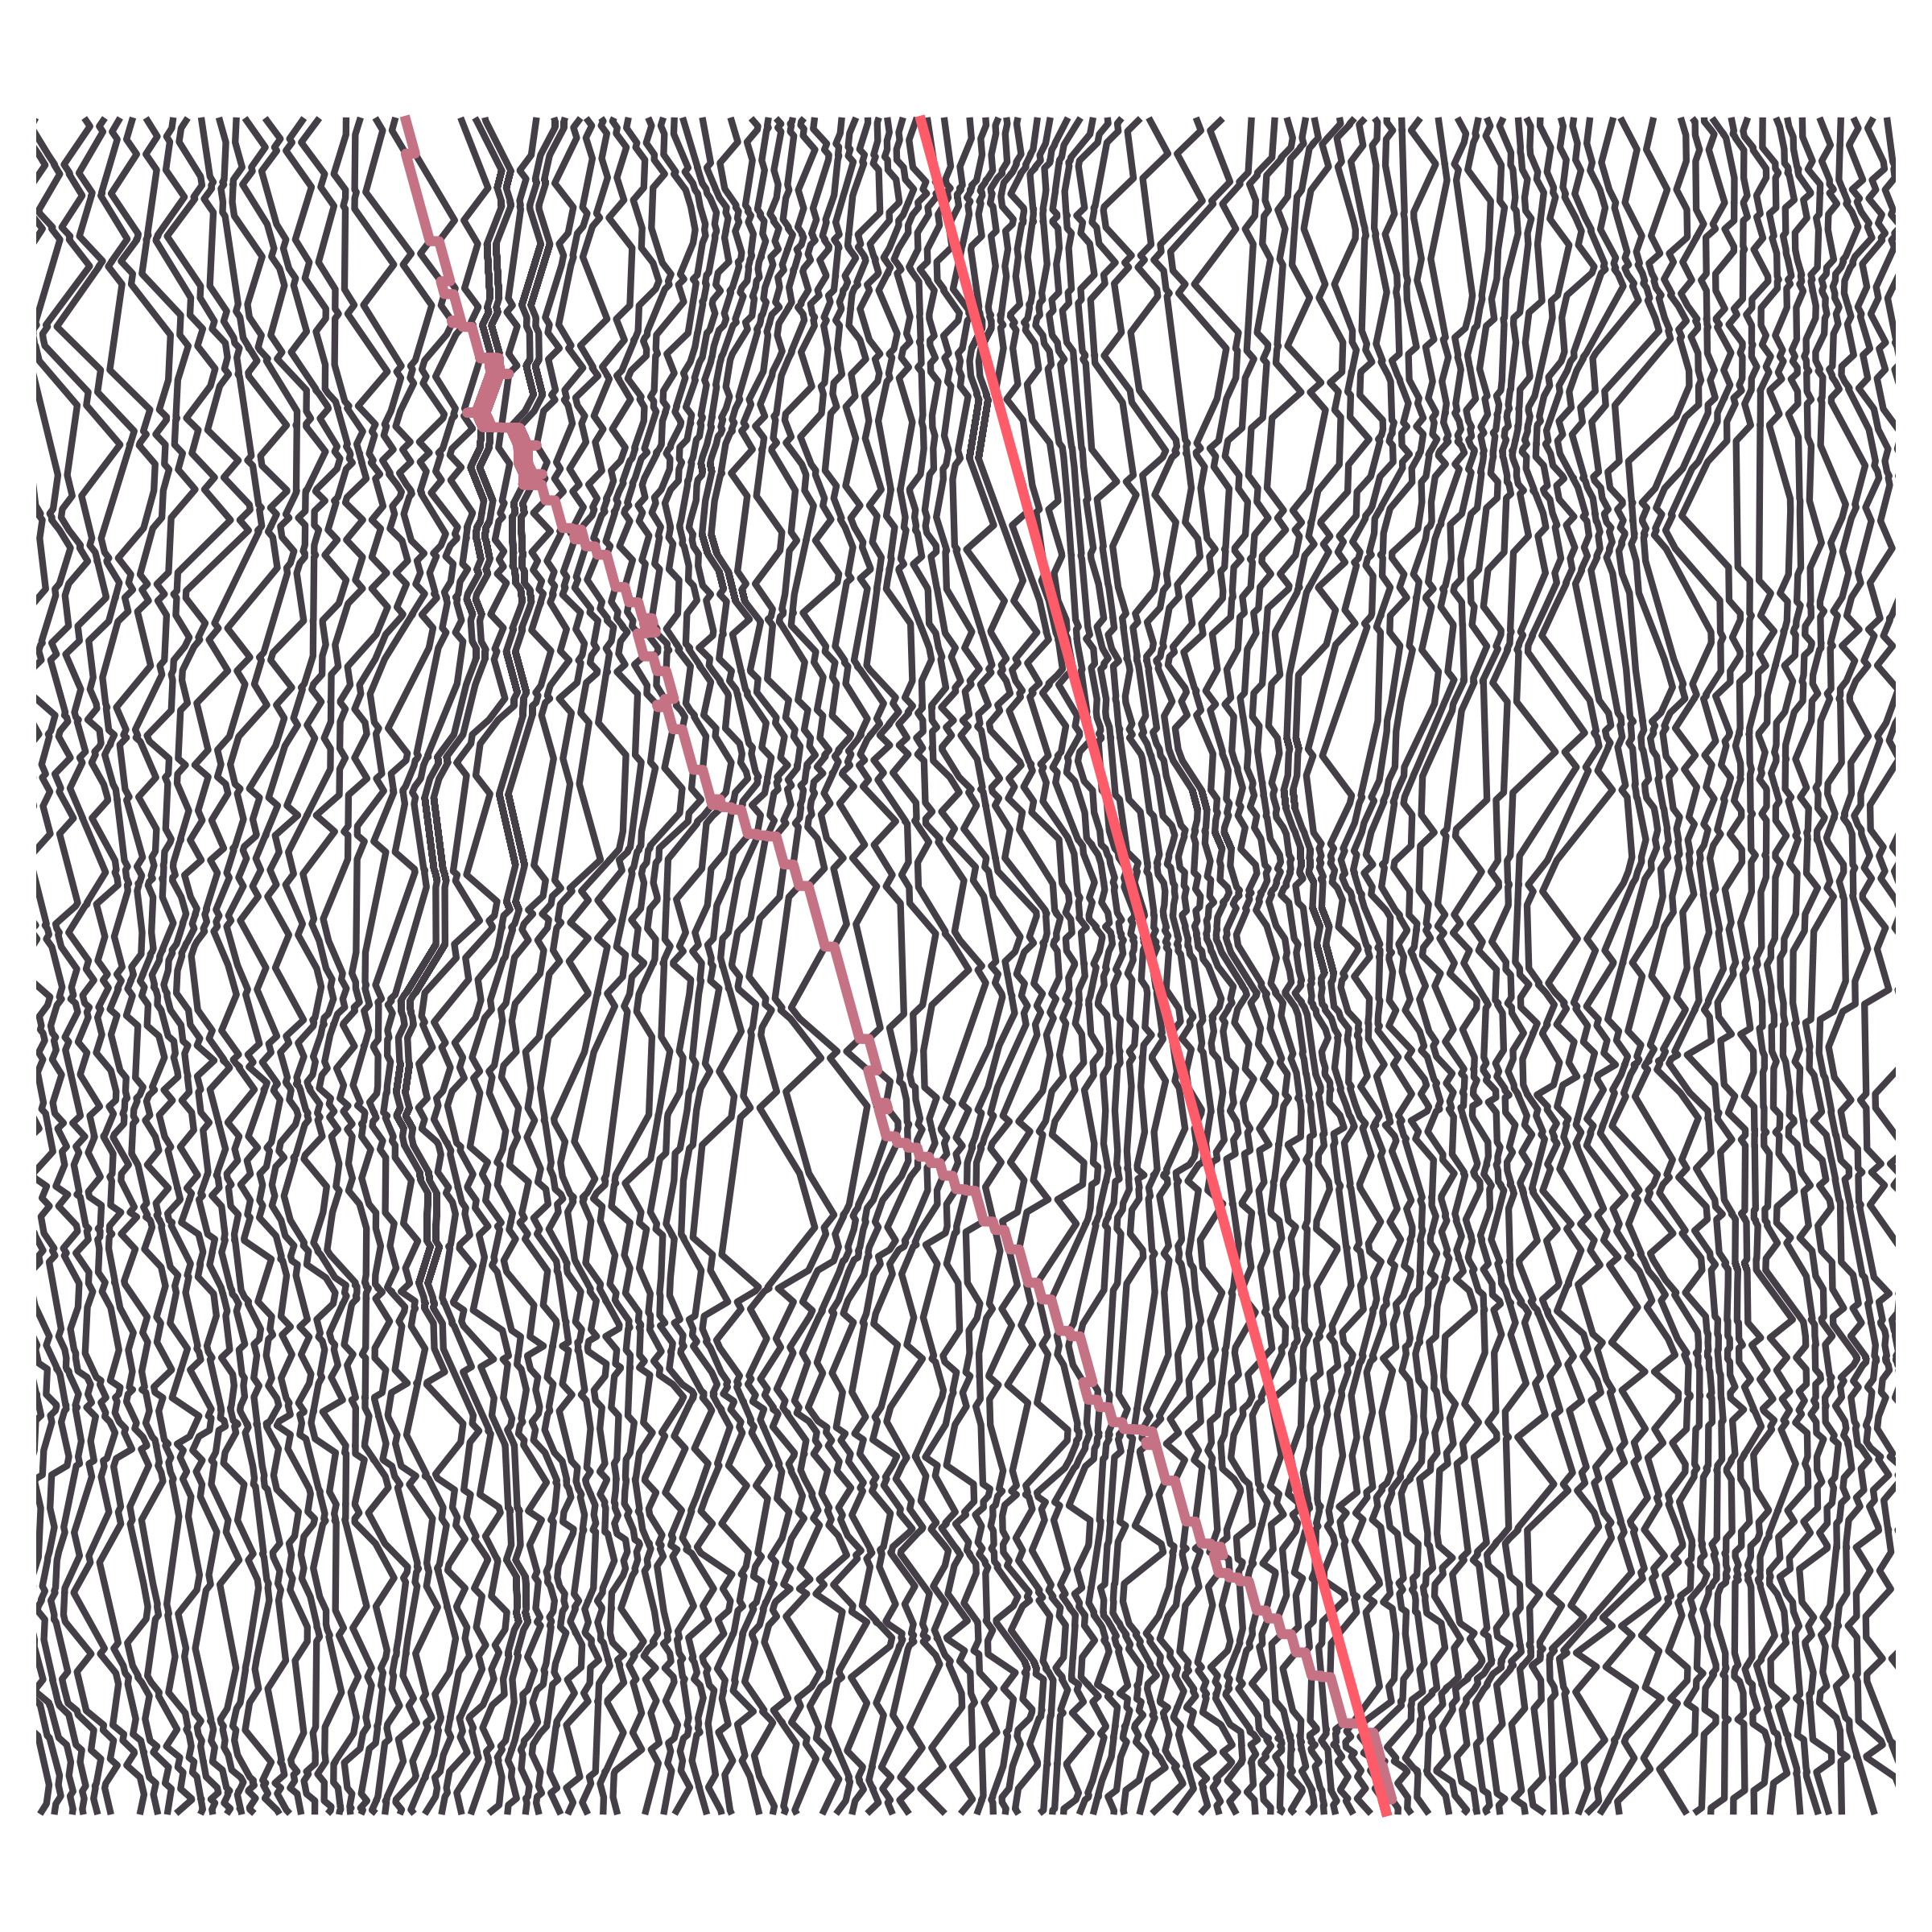
\includegraphics[width=1.0\textwidth]{trajectoires_hard_rods.png}
	};

	% Axxes 
	\draw[shift = {(-6.0,-5.5)}]
		(-1, 0) edge[thick, line width=0.5ex, ->, color=\colorOne] node[shift = {(0,0)} , pos=0.6, below]{\fontsize{12pt}{16pt}\selectfont \huge \color{\colorOne} position } (12, 0)
		(-0, -1) edge[thick, line width=0.5ex, ->, color=\colorOne] node[shift = {(0,0)} , pos=0.6, above , rotate = 90 ]{\fontsize{12pt}{16pt}\selectfont \huge \color{\colorOne} temps } (-0, 11)		
	;

	\node (pointveff) at (-3.5,5.2) {};
	\node (pointve)   at (-0.2,5.2) {};

	\draw[ opacity = 1.0 ]

	    (pointveff) edge[line width=0.4ex ,color = colorFive ,arrows = {Computer Modern Rightarrow[sharp ,length=0.2cm]-},  , out = 90 , in = 180  ]node[pos=1, right]{\color{colorFive} \fontsize{15}{10}\selectfont \bfseries  $ \displaystyle  v^{\mathrm{eff}}_{[\rho]}(v) = v + \ptFleche{motDelta}{$\Delta$} \int \ptFleche{motcolli}{\color{colorFive} $(v^{\mathrm{eff}}_{[\rho]}(w) -v^{\mathrm{eff}}_{[\rho]}(v) ) \rho ( w ) \, d w$ }  $ }($(pointveff) + (1cm,1.75cm)$)

        (pointve) edge[line width=0.4ex ,color = colorSix ,arrows = {Computer Modern Rightarrow[sharp ,length=0.2cm]-},  , out = 90 , in = 180  ]node[pos=1, right]{\color{colorSix} \fontsize{15}{10}\selectfont \bfseries  $ \displaystyle  v $ }($(pointve) + (1cm,0.75cm)$)

		(motDelta) edge[line width=0.4ex ,color = colorSix ,arrows = {Computer Modern Rightarrow[sharp ,length=0.2cm]-},  , out = 90 , in = 0  ]node[pos=1, left]{\color{colorSix} \fontsize{10}{10}\selectfont \bfseries  - diameters of balls }($(motDelta) + (-1cm,1.0cm)$)

		(motcolli) edge[line width=0.4ex ,color = colorSix ,arrows = {Computer Modern Rightarrow[sharp ,length=0.2cm]-},  , out = -150 , in = 150  ]node[pos=1, right]{\color{colorSix} \fontsize{10}{10}\selectfont \bfseries  number of collisions per second }($(motcolli) + (-1cm,-1.0cm)$)


	;

	%\drawgrid{-7}{7}{-7}{7}

\end{tikzpicture}

% veff quqntique 
\begin{tikzpicture}

	\draw[shift = {(0,-0)}]
		(-1, 0) edge[thick, line width=0.5ex, ->, color=\colorOne] node[shift = {(0,0)} , pos=1.0, right]{\fontsize{12pt}{16pt}\selectfont \huge \color{\colorOne} $x$ } (7, 0)
		(-1, 5) edge[thick, line width=0.5ex, ->, color=\colorOne] node[shift = {(0,0)} , pos=1.0, right]{\fontsize{12pt}{16pt}\selectfont \huge \color{\colorOne} $x$ } (7, 5)
		(-0, -1) edge[thick, line width=0.5ex, ->, color=\colorOne] node[shift = {(0,0)} , pos=0.5, above , rotate = 90 ]{\fontsize{12pt}{16pt}\selectfont \huge \color{\colorOne} time } (-0, 6)		
	;

	\draw[shift = {(0,-0)}]
		(3,-0.2) edge[thick, line width=0.5ex, color=\colorFive](3,0.2)
		(4,-0.2) edge[thick, line width=0.5ex, color=\colorFive](4,0.2)
	;

	

	\draw[
        decoration={
			markings,
			mark connection node=my node,
            mark=at position 0.5 with {
                \node[
                    color=\colorThree,
                    transform shape,
					draw = none ,
					rectangle,
					fill = colorTwo
                ] (my node) {
					\fontsize{15}{5}\selectfont \bfseries \color{\colorThree} $ L $
				};
            },
        },
        %postaction={decorate},
        color=\colorThree,
        thick,
        line width=0.5ex,
		shift = {(0,-0.5)}
        ] 
		(3, 0) edge[arrows={Computer Modern Rightarrow[line cap=round]-}] (3.2, 0) decorate {(3.2, 0) -- (3.8, 0)} (3.8, 0) edge[arrows={-Computer Modern Rightarrow[line cap=round]}] (4, 0)
	;

	\draw[
        decoration={
			markings,
			mark connection node=my node,
            mark=at position 0.5 with {
                \node[
                    color=\colorFour,
                    transform shape,
					draw = none ,
					rectangle,
					fill = colorTwo,
					%rotate = 90
                ] (my node) {
					\fontsize{10}{5}\selectfont \bfseries \color{\colorFour}  Interaction
				};
            },
        },
        %postaction={decorate},
        color=\colorFour,
        thick,
        line width=0.5ex,
		shift = {(8,0)}
        ] 
		(0, 0) edge[arrows={Computer Modern Rightarrow[line cap=round]-}] (0, 0.2) decorate {(0,0.2) -- (0, 2.8)} (0, 2.8) edge[arrows={-Computer Modern Rightarrow[line cap=round]}] (0, 3)
	;

	\draw[
        decoration={
			markings,
			mark connection node=my node,
            mark=at position 0.5 with {
                \node[
                    color=\colorFour,
                    transform shape,
					draw = none ,
					rectangle,
					fill = colorTwo,
					%rotate = 90
                ] (my node) {
					\fontsize{5}{5}\selectfont \bfseries \color{\colorFour} \begin{tabular}{c} no \\[0.01cm] interaction \end{tabular}  
				};
            },
        },
        %postaction={decorate},
        color=\colorFour,
        thick,
        line width=0.5ex,
		shift = {(8,3)}
        ] 
		(0, 0) edge[arrows={Computer Modern Rightarrow[line cap=round]-}] (0, 0.2) decorate {(0,0.2) -- (0, 1.8)} (0, 1.8) edge[arrows={-Computer Modern Rightarrow[line cap=round]}] (0, 2)
	;

	\node[] (v1) at (3.8,0) {
		\tikz \shade[draw = none , inner color = colorFour , outer color=colorTwo, opacity = 0.8 , shading=radial ] (0,0) circle (0.2) ;
	};
	\node[] (v2) at (3.9,0) {
		\tikz \shade[draw = none , inner color = colorFour , outer color=colorTwo, opacity = 0.8 , shading=radial ] (0,0) circle (0.2) ;
	};
	\node[] (v3) at (3.4,0) {
		\tikz \shade[draw = none , inner color = colorFour , outer color=colorTwo, opacity = 0.8 , shading=radial ] (0,0) circle (0.2) ;
	};
	\node[] (v4) at (3.5,0) {
		\tikz \shade[draw = none , inner color = colorFour , outer color=colorTwo, opacity = 0.8 , shading=radial ] (0,0) circle (0.2) ;
	};
	\node[] (v5) at (3.2,0) {
		\tikz \shade[draw = none , inner color = colorFour , outer color=colorTwo, opacity = 0.8 , shading=radial ] (0,0) circle (0.2) ;
	};

	\begin{scope}[shift = {(0,5)}]
	\node[] (v12) at (0.5,0) {
		\tikz \shade[draw = none , inner color = colorFour , outer color=colorTwo, opacity = 0.8 , shading=radial ] (0,0) circle (0.2); 
			
	};
	\node[] (v22) at (2,0) {
		\tikz \shade[draw = none , inner color = colorFour , outer color=colorTwo, opacity = 0.8 , shading=radial ] (0,0) circle (0.2) ; 
	};
	\node[] (v32) at (3,0) {
		\tikz \shade[draw = none , inner color = colorFour , outer color=colorTwo, opacity = 0.8 , shading=radial ] (0,0) circle (0.2) ;
	};
	\node[] (v42) at (5,0) {
		\tikz \shade[draw = none , inner color = colorFour , outer color=colorTwo, opacity = 0.8 , shading=radial ] (0,0) circle (0.2) ;
	};
	\node[] (v52) at (6.5,0) {
		\tikz \shade[draw = none , inner color = colorFour , outer color=colorTwo, opacity = 0.8 , shading=radial ] (0,0) circle (0.2) ;
	};
	\node [above = 0mm of v12 , shift = {(0,0mm)}]{\color{colorFour}\fontsize{12pt}{16pt}\selectfont $\theta_1$} ;
	\node [above = 0mm of v22 , shift = {(0,0mm)}]{\color{colorFour}\fontsize{12pt}{16pt}\selectfont $\theta_2$} ;
	\node [above = 0mm of v52 , shift = {(0,0mm)}]{\color{colorFour}\fontsize{12pt}{16pt}\selectfont $\theta_N$} ; 

	\end{scope}



	\draw[line width=0.4ex ,color = colorFour ,  opacity = 0.5 ]
	    (v1) edge[out = 90 , in = -50  ](v12)
		(v2) edge[out = 90 , in = -70  ](v22)
		(v3) edge[out = 90 , in = -90  ](v32)
		(v4) edge[out = 90 , in = -110  ](v42)
		(v5) edge[out = 90 , in = -140  ](v52)

	;

	\begin{scope}[shift={(3.5,2.1)} , opacity = 0.5]
    	\draw[
			draw = none ,
        	fill = colorFour,
       	 	color = colorFour,
       		decorate,
        	decoration={random steps, segment length=1mm, amplitude=1mm}
   		 ] (0,0) circle (1.6);

    	% Texte au centre
    	\node at (0,0.) {\color{colorTwo} \fontsize{10pt}{5pt}\selectfont \bf Interaction};
	\end{scope}


	%\drawgrid{-1}{7}{-1}{7}
\end{tikzpicture}

% tube 
\begin{tikzpicture}
	\draw[shift = {(0,-0)}]
		(-8, 0) edge[thick, line width=0.5ex, ->, color=\colorOne] node[shift = {(0,0)} , pos=1.0, above]{\fontsize{12pt}{16pt}\selectfont \huge \color{\colorOne} $\vec{e}_x$ } (8, 0)
		(-0, -1) edge[thick, line width=0.5ex, ->, color=\colorOne] node[shift = {(0,0)} , pos=0.8, above , rotate = 90 ]{\fontsize{12pt}{16pt}\selectfont \huge \color{\colorOne} $\vec{e}_y$ } (-0, 2)		
	;

	\draw[fill=\colorFive , opacity = 0.8 , draw = none , rounded corners = 4ex ]
		(-7.2,-0.75) rectangle (7.2,0.75)
	;
	\draw[line width=2.0ex, color=\colorFive ]
		(-7.0,-0.75) -- (7.0,-0.75)
		(-7.0,0.75) -- (7.0,0.75)
	;
\end{tikzpicture}

% harmonique transv exité
\begin{tikzpicture}

	\begin{scope}[shift = {(-6,-0)}]
		%\node[] (A) {
			%\begin{tikzpicture}
				\draw[shift = {(-0.5,-0)}, fill=colorFive , opacity = 0.8 , draw = colorOne , rounded corners = 0ex , thick, line width=0.5ex, ]
					(0,0) rectangle (1,5)
				;
				\draw[shift = {(-0.5,3.5)},opacity = 1.0 , draw = colorSix , thick, line width=0.8ex, scale = 1.0 ]
					(-0.2,0) -- (1.2,0)
				;
			%\end{tikzpicture}
		%};
		% \node[above = of (-5,7)]  { \fontsize{12pt}{16pt}\selectfont \huge \color{\colorFour}  Temperature T
		% }	
		% ;
		\node[]  at (0,6) {\fontsize{15}{5}\selectfont \bfseries \color{\colorFour}  Energy/Atom};
	\end{scope}

	\begin{scope}[shift = {(0,-0)}]
		% Points donnés
    	\pgfmathsetmacro{\xA}{-2}
    	\pgfmathsetmacro{\yA}{3}
    	\pgfmathsetmacro{\xB}{0}
    	\pgfmathsetmacro{\yB}{0}
    	\pgfmathsetmacro{\xC}{2}
    	\pgfmathsetmacro{\yC}{3}

    	% Résolution du système pour la parabole y = a*x^2 + b*x + c
    	\pgfmathsetmacro{\den}{(\xA-\xB)*(\xA-\xC)*(\xB-\xC)}
    	\pgfmathsetmacro{\a}{(\xC*(\yB-\yA)+\xB*(\yA-\yC)+\xA*(\yC-\yB))/\den}
    	\pgfmathsetmacro{\b}{(\xC*\xC*(\yA-\yB)+\xB*\xB*(\yC-\yA)+\xA*\xA*(\yB-\yC))/\den}
    	\pgfmathsetmacro{\c}{(\xB*\xC*(\xB-\xC)*\yA+\xC*\xA*(\xC-\xA)*\yB+\xA*\xB*(\xA-\xB)*\yC)/\den}

    	% Axes
    	%\draw[->] (-3,0) -- (3,0) node[right] {$x$};
    	%\draw[->] (0,-0.5) -- (0,4) node[above] {$V(x)$};

    	% Parabole ajustée
    	\draw[domain=-2.5:2.5, smooth, variable=\x, thick, line width=0.8ex, color = colorOne ]
        	plot ({\x},{\a*\x*\x + \b*\x + \c});

    	% Points donnés
    	%\filldraw[red] (\xA,\yA) circle (1.5pt);
    	%\filldraw[red] (\xB,\yB) circle (1.5pt);
    	%\filldraw[red] (\xC,\yC) circle (1.5pt);

		\begin{scope}[shift = {(0,-0)}]
			%\clip (-3,0) plot[domain=-2.5:2.5, smooth, variable=\x] ({\x},{\a*\x*\x + \b*\x + \c}) -- (2.5,0) -- cycle ;

			%\draw[domain=-2.5:2.5, smooth, variable=\x, thick, line width=0.8ex, color = colorOne ](-4,0) -- (-4,5) --  plot ({\x},{\a*\x*\x + \b*\x + \c}) -- (4,5) -- (4,0) -- cycle ;

			%\clip (-4,0) -- (-4,5) --  plot[domain=-2.5:2.5, smooth, variable=\x] ({\x},{\a*\x*\x + \b*\x + \c}) -- (4,5) -- (4,0) -- cycle ;

			\clip plot[domain=-2.5:2.5, smooth, variable=\x] ({\x},{\a*\x*\x + \b*\x + \c}) -- cycle ;

			\begin{scope}[shift = {(-3, 0.4)}]
				\draw[shift = {(0,0)}, line width=0.8ex, color=\colorFour , dashed] (0,0) -- (6,0);
				\draw[shift = {(0,1)}, line width=0.8ex, color=\colorFour!75!\colorSix , dashed] (0,0) -- (6,0);	
				\draw[shift = {(0,2)}, line width=0.8ex, color=\colorFour!50!\colorSix , dashed] (0,0) -- (6,0);	
				\draw[shift = {(0,3)}, line width=0.8ex, color=\colorFour!25!\colorSix , dashed] (0,0) -- (6,0);	
				\draw[shift = {(0,4)}, line width=0.8ex, color=\colorSix , dashed] (0,0) -- (6,0);		
			\end{scope}
		\end{scope}


		\draw[
        decoration={
			markings,
			mark connection node=my node,
            mark=at position 0.5 with {
                \node[
                    color=\colorFour,
                    transform shape,
					draw = none ,
					rectangle,
					fill = colorTwo,
					%rotate = 90
                ] (my node) {
					\fontsize{10}{5}\selectfont \bfseries \color{\colorFour}  \begin{tabular}{c} Excited \\[0.01cm] states \end{tabular} 
				};
            },
        },
        %postaction={decorate},
        color=\colorFour,
        thick,
        line width=0.5ex,
		shift = {(3,1.2)}
        ] 
		(0, 0) edge[arrows={Computer Modern Rightarrow[line cap=round]-}] (0, 0.2) decorate {(0,0.2) -- (0, 3.3)} (0, 3.3) edge[arrows={-Computer Modern Rightarrow[line cap=round]}] (0, 3.5)
		;

		\draw[
			color=\colorFour,
        	thick,
        	line width=0.5ex,
			shift = {(1.5,0.4)}
			]
			(0, 0) edge[arrows={Computer Modern Rightarrow[line cap=round]-Computer Modern Rightarrow[line cap=round]}]node[pos = 0.5 , right ]{\fontsize{8}{5}\selectfont \bfseries \color{\colorFour} $\Delta E_\perp = \hbar \omega_\perp $} (0, 1)
		;

		\draw[
			color=\colorFour,
        	thick,
        	line width=0.5ex,
			shift = {(0,0)}
			]
			(0, 0.35) edge[out = -50 , in = 180 , arrows={Computer Modern Rightarrow[line cap=round]-}]node[pos = 1.0, right ]{\fontsize{10}{5}\selectfont \bfseries \color{\colorFour} \begin{tabular}{c} Ground \\[0.01cm] state \end{tabular} } (2, -0.6)
		;

		\node[] at (0,6) {\fontsize{15}{5}\selectfont \bfseries \color{\colorFour} Transverse energy states };

		\begin{scope}[shift = {(0, 0.4)}]
			\draw[shift = {(-0.5, 1 )}, draw = none , inner color = colorSix , outer color=colorTwo, opacity = 0.8 , shading=radial ] (0,0) circle (0.2);
			\draw[shift = {(-1.0, 2)}, draw = none , inner color = colorSix , outer color=colorTwo, opacity = 0.8 , shading=radial ] (0,0) circle (0.2);
			\draw[shift = {(1.2, 2 )}, draw = none , inner color = colorSix , outer color=colorTwo, opacity = 0.8 , shading=radial ] (0,0) circle (0.2);
			\draw[shift = {(-1.0, 3)}, draw = none , inner color = colorSix , outer color=colorTwo, opacity = 0.8 , shading=radial ] (0,0) circle (0.2);
			\draw[shift = {(1.0, 3 )}, draw = none , inner color = colorSix , outer color=colorTwo, opacity = 0.8 , shading=radial ] (0,0) circle (0.2);
		\end{scope}
	\end{scope}

	%\drawgrid{-3}{3}{-1}{5}
\end{tikzpicture}

% harmonique transv fonda
\begin{tikzpicture}

	\begin{scope}[shift = {(-6,-0)}]
		%\node[] (A) {
			%\begin{tikzpicture}
				\draw[shift = {(-0.5,-0)}, fill=colorFive , opacity = 0.8 , draw = colorOne , rounded corners = 0ex , thick, line width=0.5ex, ]
					(0,0) rectangle (1,5)
				;
				\draw[shift = {(-0.5,0.5)},opacity = 1.0 , draw = colorSix , thick, line width=0.8ex, scale = 1.0 ]
					(-0.2,0) -- (1.2,0)
				;
			%\end{tikzpicture}
		%};
		% \node[above = of (-5,7)]  { \fontsize{12pt}{16pt}\selectfont \huge \color{\colorFour}  Temperature T
		% }	
		% ;
		\node[]  at (0,6) {\fontsize{15}{5}\selectfont \bfseries \color{\colorFour}  Energy/Atom};
	\end{scope}

	\begin{scope}[shift = {(0,-0)}]
		% Points donnés
    	\pgfmathsetmacro{\xA}{-2}
    	\pgfmathsetmacro{\yA}{3}
    	\pgfmathsetmacro{\xB}{0}
    	\pgfmathsetmacro{\yB}{0}
    	\pgfmathsetmacro{\xC}{2}
    	\pgfmathsetmacro{\yC}{3}

    	% Résolution du système pour la parabole y = a*x^2 + b*x + c
    	\pgfmathsetmacro{\den}{(\xA-\xB)*(\xA-\xC)*(\xB-\xC)}
    	\pgfmathsetmacro{\a}{(\xC*(\yB-\yA)+\xB*(\yA-\yC)+\xA*(\yC-\yB))/\den}
    	\pgfmathsetmacro{\b}{(\xC*\xC*(\yA-\yB)+\xB*\xB*(\yC-\yA)+\xA*\xA*(\yB-\yC))/\den}
    	\pgfmathsetmacro{\c}{(\xB*\xC*(\xB-\xC)*\yA+\xC*\xA*(\xC-\xA)*\yB+\xA*\xB*(\xA-\xB)*\yC)/\den}

    	% Axes
    	%\draw[->] (-3,0) -- (3,0) node[right] {$x$};
    	%\draw[->] (0,-0.5) -- (0,4) node[above] {$V(x)$};

    	% Parabole ajustée
    	\draw[domain=-2.5:2.5, smooth, variable=\x, thick, line width=0.8ex, color = colorOne ]
        	plot ({\x},{\a*\x*\x + \b*\x + \c});

    	% Points donnés
    	%\filldraw[red] (\xA,\yA) circle (1.5pt);
    	%\filldraw[red] (\xB,\yB) circle (1.5pt);
    	%\filldraw[red] (\xC,\yC) circle (1.5pt);

		\begin{scope}[shift = {(0,-0)}]
			%\clip (-3,0) plot[domain=-2.5:2.5, smooth, variable=\x] ({\x},{\a*\x*\x + \b*\x + \c}) -- (2.5,0) -- cycle ;

			%\draw[domain=-2.5:2.5, smooth, variable=\x, thick, line width=0.8ex, color = colorOne ](-4,0) -- (-4,5) --  plot ({\x},{\a*\x*\x + \b*\x + \c}) -- (4,5) -- (4,0) -- cycle ;

			%\clip (-4,0) -- (-4,5) --  plot[domain=-2.5:2.5, smooth, variable=\x] ({\x},{\a*\x*\x + \b*\x + \c}) -- (4,5) -- (4,0) -- cycle ;

			\clip plot[domain=-2.5:2.5, smooth, variable=\x] ({\x},{\a*\x*\x + \b*\x + \c}) -- cycle ;

			\begin{scope}[shift = {(-3, 0.4)}]
				\draw[shift = {(0,0)}, line width=0.8ex, color=\colorFour , dashed] (0,0) -- (6,0);
				\draw[shift = {(0,1)}, line width=0.8ex, color=\colorFour!75!\colorSix , dashed] (0,0) -- (6,0);	
				\draw[shift = {(0,2)}, line width=0.8ex, color=\colorFour!50!\colorSix , dashed] (0,0) -- (6,0);	
				\draw[shift = {(0,3)}, line width=0.8ex, color=\colorFour!25!\colorSix , dashed] (0,0) -- (6,0);	
				\draw[shift = {(0,4)}, line width=0.8ex, color=\colorSix , dashed] (0,0) -- (6,0);		
			\end{scope}
		\end{scope}


		\draw[
        decoration={
			markings,
			mark connection node=my node,
            mark=at position 0.5 with {
                \node[
                    color=\colorFour,
                    transform shape,
					draw = none ,
					rectangle,
					fill = colorTwo,
					%rotate = 90
                ] (my node) {
					\fontsize{10}{5}\selectfont \bfseries \color{\colorFour}  \begin{tabular}{c} Excited \\[0.01cm] states \end{tabular} 
				};
            },
        },
        %postaction={decorate},
        color=\colorFour,
        thick,
        line width=0.5ex,
		shift = {(3,1.2)}
        ] 
		(0, 0) edge[arrows={Computer Modern Rightarrow[line cap=round]-}] (0, 0.2) decorate {(0,0.2) -- (0, 3.3)} (0, 3.3) edge[arrows={-Computer Modern Rightarrow[line cap=round]}] (0, 3.5)
		;

		\draw[
			color=\colorFour,
        	thick,
        	line width=0.5ex,
			shift = {(1.5,0.4)}
			]
			(0, 0) edge[arrows={Computer Modern Rightarrow[line cap=round]-Computer Modern Rightarrow[line cap=round]}]node[pos = 0.5 , right ]{\fontsize{8}{5}\selectfont \bfseries \color{\colorFour} $\Delta E_\perp = \hbar \omega_\perp $} (0, 1)
		;

		\draw[
			color=\colorFour,
        	thick,
        	line width=0.5ex,
			shift = {(0,0)}
			]
			(0, 0.35) edge[out = -50 , in = 180 , arrows={Computer Modern Rightarrow[line cap=round]-}]node[pos = 1.0, right ]{\fontsize{10}{5}\selectfont \bfseries \color{\colorFour} \begin{tabular}{c} Ground \\[0.01cm] state \end{tabular} } (2, -0.6)
		;

		\node[] at (0,6) {\fontsize{15}{5}\selectfont \bfseries \color{\colorFour} Transverse energy states };

		\begin{scope}[shift = {(0, 0.4)}]
			\draw[shift = {(-0, 0 )}, draw = none , inner color = colorSix , outer color=colorTwo, opacity = 0.8 , shading=radial ] (0,0) circle (0.2);
		\end{scope}
	\end{scope}

	%\drawgrid{-3}{3}{-1}{5}
\end{tikzpicture}

%coupe puce
\begin{tikzpicture}


\begin{scope}


	% \draw[shift={(-2cm , 1.25cm)} , thick,line width=2.5cm, color = \colorThree , opacity = 1 ]
	% 	(0,0) -- node[shift={(-0.75cm , -0.5cm)} , pos = 0.0, right , color = \colorTwo]{{\color{\colorTwo} \fontsize{15pt}{8pt}\selectfont \bf SiC} } (13.5,0)
	% ;
	% \draw[shift={(-2cm , 3.5cm)} , thick,line width=2.cm, color = \colorFour , opacity = 1 ]
	% 	(0,0) -- node[shift={(-0.75cm , -0.5cm)} , pos = 0.0, right , color = \colorTwo]{{\color{\colorTwo} \fontsize{15pt}{8pt}\selectfont \bf BCB} } (13.5,0)
	% ;
	\draw[shift={(-2cm , 1.25cm)} , thick,line width=2.5cm, color = \colorThree , opacity = 1 ]
		(0,0) -- (13.5,0)
	;
	\draw[shift={(-2cm , 3.5cm)} , thick,line width=2.cm, color = \colorFour , opacity = 1 ]
		(0,0) -- (13.5,0)
	;

	\draw[shift={(-2cm , 5.cm)} , thick,line width=1.cm, color = \colorGold , opacity = 1 ]
		(0,0) -- node[shift={(-0.2cm , 0.cm)} , pos = 0.0, right , color = \colorTwo]{{\color{\colorOne} \fontsize{15pt}{8pt}\selectfont \bf Au} } (13.5,0)
	;
	
	
	\begin{scope}[shift={(2cm , 2.5cm)}]
		\draw[thick,line width=0.1cm , rounded corners=0cm,  color = \colorTwo , fill = \colorFive ] 
			(0,0) rectangle (1,1)
			;
		% croix
		\draw[ thick,line width=0.1cm , color = \colorOne] 
			(0,0) -- (1,1)
			(0,1) -- (1,0)
		;
		\node[left , shift={(-0.3cm , 0.5cm)} , color = \colorTwo] at (0,0) {{\color{\colorTwo}\fontsize{20pt}{8pt}\selectfont$-I$}};
	\end{scope}
	
	\begin{scope}[shift={(5cm , 2.5cm)}]
		\draw[thick,line width=0.1cm , rounded corners=0cm,  color = \colorTwo , fill = \colorFive ] 
			(0,0) rectangle (1,1)
			;
		% croix
		\fill[ thick,line width=0.1cm , color = \colorOne] 
			(0.5,0.5) circle (0.1cm);
		\node[left , shift={(-0.3cm , 0.5cm)} , color = \colorTwo] at (0,0) {{\color{\colorTwo}\fontsize{20pt}{8pt}\selectfont$I$}};
	\end{scope}
	
	\begin{scope}[shift={(8cm , 2.5cm)}]
		\draw[thick,line width=0.1cm , rounded corners=0cm,  color = \colorTwo , fill = \colorFive ] 
			(0,0) rectangle (1,1)
			;
		% croix
		\draw[ thick,line width=0.1cm , color = \colorOne] 
			(0,0) -- (1,1)
			(0,1) -- (1,0)
		;
		\node[left , shift={(-0.3cm , 0.5cm)} , color = \colorTwo] at (0,0) {{\color{\colorTwo}\fontsize{20pt}{8pt}\selectfont$-I$}};
	\end{scope}
	
	\draw[shift={(2.5cm , 2.cm)}]
		(0,0) edge [decoration={
   							markings,
    						mark connection node=midnode,
    						mark=at position 0.5 with {
      							\node[draw = none ,fill= \colorThree ,transform shape , opacity = 1] (midnode) {{\color{\colorTwo} \fontsize{10pt}{8pt}\selectfont
					$d = 15 \mu m $}};
    							}
 						 	},
  							postaction={decorate},
		thick,line width=0.1cm , <->, color = \colorTwo	, >=Stealth	
		] (3,0)
	;
	
	\draw[shift={(3.8cm , 3.cm)}]
		(0,0) edge [decoration={
   							markings,
    						mark connection node=midnode,
    						mark=at position 0.5 with {
      							\node[draw = none ,fill= \colorGold ,transform shape , opacity = 1] (midnode) {{\color{\colorOne} \fontsize{20pt}{8pt}\selectfont
					$d$}};
    							}
 						 	},
  							postaction={decorate},
		thick,line width=0.1cm , <->, color = \colorOne , >=Stealth	
		] (0,3.6)
	;
	
	% \draw[shift={(10.25cm , 0.cm)}]
	% 	(0,0) edge [decoration={
   	% 						markings,
    % 						mark connection node=midnode,
    % 						mark=at position 0.5 with {
    %   							\node[draw = none ,fill= \colorThree ,transform shape , opacity = 1] (midnode) {{\color{\colorTwo} \fontsize{10pt}{8pt}\selectfont
	% 				$\sim 300 \mu m $}};
    % 							}
 	% 					 	},
  	% 						postaction={decorate},
	% 	thick,line width=0.1cm , <->, color = \colorTwo	, >=Stealth	
	% 	] (0,2.5)
	% ;
	
	% \draw[shift={(10.25cm , 2.5cm)}]
	% 	(0,0) edge [decoration={
   	% 						markings,
    % 						mark connection node=midnode,
    % 						mark=at position 0.5 with {
    %   							\node[draw = none ,fill= \colorFour ,transform shape , opacity = 1] (midnode) {{\color{\colorTwo} \fontsize{10pt}{8pt}\selectfont
	% 				$< 6 \,\mu m $}};
    % 							}
 	% 					 	},
  	% 						postaction={decorate},
	% 	thick,line width=0.1cm , <->, color = \colorTwo	, >=Stealth	
	% 	] (0,2)
	% ;
	
	% \draw[shift={(10.25cm , 4.5cm)}, thick,line width=0.1cm , {Triangle[scale=0.5]}-{Triangle[scale=0.5]}, color = \colorOne ]
	% 	(0,0) -- node[pos = 0.5 , left ]{{\color{\colorOne} \fontsize{15pt}{8pt}\selectfont $\sim 150 \, nm $}}  (0,1)
	% ;
	
	\draw[shift={(2.5cm , 5.5cm)}, thick,line width=0.08cm , >-< ,   {Triangle[scale=0.7, reversed]}-{Triangle[scale=0.7, reversed]}, color = \colorOne ]
		(0,0) -- node[pos = 0.5 , left ]{{\color{\colorOne} \fontsize{17pt}{8pt}\selectfont $\sim 7 \,\mu m $}}  (0,1.1)
	;
	
	\begin{scope}[shift={(4.5cm , 5.5cm)} , decoration={
    		markings,% switch on markings
    		mark=between positions 0.3 and 1 step 1cm with {\arrow[\colorSix,line width=1mm]{>}}}
    	]
  		\draw [postaction={decorate} , color = \colorSix , line width=1mm] (0,0) .. controls (1,1) and (1,1) .. (2,0);
  		\draw [ shift={(2.25cm , 2.25cm)} , rotate = 90, xscale=-1 ,  postaction={decorate} , color = \colorSix , line width=1mm] (0,0) .. controls (1,1) and (1,1) .. (2,0);
  		\draw [shift={(-0.25cm , 0.25cm)} , rotate = -90, xscale=-1 , postaction={decorate} , color = \colorSix , line width=1mm] (0,0) .. controls (1,1) and (1,1) .. (2,0);
  		\draw [shift={(2.cm , 2.5cm)} , rotate = 180, xscale=1 , postaction={decorate} , color = \colorSix , line width=1mm] (0,0) .. controls (1,1) and (1,1) .. (2,0);
  		
  		\node[align=center, font=\fontsize{15}{12}\selectfont, text=\colorSix] at (3.95,1.25) {Field produced \\ by the micro-wires};
	\end{scope}
	

	\draw[shift={(-0.0cm , -0.0cm)} , thick,line width=0.1cm, color = \colorOne , opacity = 1 ]
		(-0.,0)edge[, ->] node[pos = 1.01, above]{\fontsize{20pt}{8pt}\selectfont$\bm{\vec{e}_u}$} (12,0)
		(0,-0.) edge[, ->] node[pos = 0.99, left]{\fontsize{20pt}{8pt}\selectfont$\bm{\vec{e}_v}$} (0,7.25)
	;
	
	\draw[thick ,line width=0.1cm] (0,0) circle (0.3cm);
	\fill (0,0) circle (1mm);
	\node[below , shift={(-0.0cm , -0.4cm)}] at (0,0) {\fontsize{20pt}{8pt}\selectfont$\bm{\vec{e}_x}$};
	
	
	
	%\drawgrid{-3}{12}{-1}{10}
\end{scope}
\end{tikzpicture}

% bipartition Oms
\begin{tikzpicture}
	\draw[shift = {(0,-0)}]
		(-2, 0) edge[thick, line width=0.5ex, ->, color=\colorOne] node[shift = {(0,0)} , pos=1.0, above]{\fontsize{12pt}{16pt}\selectfont \huge \color{\colorOne} $x$ } (3, 0)
		(-0, -0.5) edge[thick, line width=0.5ex, ->, color=\colorOne] node[shift = {(0,0)} , pos=0.8, above , rotate = 90 ]{\fontsize{12pt}{16pt}\selectfont \huge \color{\colorOne} $n(x)$ } (-0, 3)		
	;

	% Zone remplie
\fill[
    shift={(0,0)},
    color=\colorFour,
    ultra thick,
    line width=0.6ex,
	opacity = 0.6
]
(-1.5,0) -- (0,0) -- (0,2) -- (3,2) -- (3,0) -- cycle;

\draw[
    shift={(0,0)},
    fill=none,
    color=\colorFour,
    ultra thick,
    line width=0.6ex
]
(-1.5,0) -- (0,0) -- (0,2) -- (2,2);

% Prolongement pointillé
\draw[
    color=\colorFour,
    ultra thick,
    line width=0.6ex,
    dashed
]
(2,2) -- (3,2);



\end{tikzpicture}


% bipartition tms
\begin{tikzpicture}[use Hobby shortcut]
	\draw[shift = {(0,-0)}]
		(-2, 0) edge[thick, line width=0.5ex, ->, color=\colorOne] node[shift = {(0,0)} , pos=1.0, above]{\fontsize{12pt}{16pt}\selectfont \huge \color{\colorOne} $x$ } (3, 0)
		(-0, -0.5) edge[thick, line width=0.5ex, ->, color=\colorOne] node[shift = {(0,0)} , pos=0.8, above , rotate = 90 ]{\fontsize{12pt}{16pt}\selectfont \huge \color{\colorOne} $n(x)$ } (-0, 3)		
	;

	% Zone remplie
% Zone remplie semi-transparente
\fill[
    shift={(0,0)},
    fill=\colorFour,
    opacity=0.6
]
(-1.5,0) -- (-1,0) .. controls (0,0) and (0,2) .. (1,2) -- (3,2) -- (3,0) -- cycle;

% Contour plein jusqu'à (2,2)
\draw[
    shift={(0,0)},
    color=\colorFour,
    line width=0.6ex,
    line cap=round,
    line join=round
]
(-1.5,0) -- (-1,0) .. controls (0,0) and (0,2) .. (1,2) -- (2,2);

% Prolongement pointillé à partir de (2,2)
\draw[
    color=\colorFour,
    line width=0.6ex,
    line cap=round,
    dashed
]
(2,2) -- (3,2);

\end{tikzpicture}


%potentiel 4 
\begin{tikzpicture}[use Hobby shortcut]

	\begin{scope}[shift = {(0,-0)}]
		\draw[shift = {(0,-0)}]
			(-3, 0) edge[thick, line width=0.5ex, ->, color=\colorOne] node[shift = {(0,0)} , pos=1.0, below]{\fontsize{12pt}{16pt}\selectfont \huge \color{\colorOne} $x$ } (3, 0)	
		;
		\def\a{0.05}
		\def\xmax{2.5}	

		\draw[domain=-2.7:2.7, smooth, variable=\x, thick, line width=0.8ex, color = colorOne ]
        	plot ({\x},{\a*\x*\x*\x*\x}  );

		\draw[domain=-\xmax:\xmax, smooth, variable=\x, thick, line width=0.8ex, color = colorFour ]
        	plot ({\x},{-\a*\x*\x*\x*\x  + \a*\xmax^4 } );

	
		\draw[line width=0.8ex, color = colorSix , fill = colorFive , opacity = 0.7 ] (-2.8, 0 ) rectangle (-1,2.3) ; 


		\draw[opacity = 1.0 ]
            (0,0) edge[shift = {(-2,-0.1)}, line width=0.4ex ,color = colorSix ,arrows = {Computer Modern Rightarrow[sharp ,length=0.2cm]-},  , out = -90 , in = 180 ]node[pos=1, right ]{\color{colorSix} \fontsize{20pt}{10pt}\selectfont \bfseries  light beams  }($(0,0) + (0.5cm,-0.75cm)$)

			(0,0) edge[shift = {(2.6,2.5)}, line width=0.4ex ,color = colorOne ,arrows = {Computer Modern Rightarrow[sharp ,length=0.2cm]-},  , out = 150 , in = 0 ]node[pos=1, left ]{\color{colorOne} \fontsize{20pt}{10pt}\selectfont \bfseries  \begin{tabular}{r}potential \\ $V_\parallel(x) \propto x^4 $ \end{tabular}  }($(0,0) + (-1.25cm,1.75cm)$)

			(0,0) edge[shift = {(0,2.1)}, line width=0.4ex ,color = colorFour ,arrows = {Computer Modern Rightarrow[sharp ,length=0.2cm]-},  , out = 130, in = 0 ]node[pos=1, left ]{\color{colorFour} \fontsize{20pt}{10pt}\selectfont \bfseries  density $n(x)$ }($(0,0) + (-1.0cm,0.75cm)$)
	    ;
	\end{scope}

	\begin{scope}[shift = {(4.8,-0)}]
		\node[rectangle] at (0,1) {\color{colorFour} \fontsize{40}{10}\selectfont \bfseries  $\Rightarrow$ } ;
	\end{scope}



	\begin{scope}[shift = {(9,-0)}]
		\draw[shift = {(0,-0)}]
			(-3, 0) edge[thick, line width=0.5ex, ->, color=\colorOne] node[shift = {(0,0)} , pos=1.0, below]{\fontsize{12pt}{16pt}\selectfont \huge \color{\colorOne} $x$ } (3, 0)	
		;
		\def\a{0.05}
		\def\xmax{2.5}	

		%\draw[domain=-2.7:2.7, smooth, variable=\x, thick, line width=0.8ex, color = colorOne ]plot ({\x},{\a*\x*\x*\x*\x}  );

		\draw[line width=0.8ex, color = colorFour ]
        	(-3,0) -- (-1,0) -- plot[domain=-1:\xmax, smooth, variable=\x] ({\x},{-\a*\x*\x*\x*\x  + \a*\xmax^4 } ) -- (3,0);

	
%		\draw[line width=0.8ex, color = colorSix , fill = colorFive , opacity = 0.7 ] (-2.8, 0 ) rectangle (-1,2.3) ; 


		\draw[opacity = 1.0 ]
            %(0,0) edge[shift = {(-2,-0.1)}, line width=0.4ex ,color = colorSix ,arrows = {Computer Modern Rightarrow[sharp ,length=0.2cm]-},  , out = -90 , in = 0 ]node[pos=1, left ]{\color{colorSix} \fontsize{10}{10}\selectfont \bfseries  light beams  }($(0,0) + (-0.5cm,-0.75cm)$)

			%(0,0) edge[shift = {(2.6,2.5)}, line width=0.4ex ,color = colorOne ,arrows = {Computer Modern Rightarrow[sharp ,length=0.2cm]-},  , out = 150 , in = 0 ]node[pos=1, left ]{\color{colorOne} \fontsize{10}{10}\selectfont \bfseries  \begin{tabular}{r}potential \\ $V_\parallel(x) \propto x^4 $ \end{tabular}  }($(0,0) + (-1.0cm,0.75cm)$)

			(0,0) edge[shift = {(0,2.1)}, line width=0.4ex ,color = colorFour ,arrows = {Computer Modern Rightarrow[sharp ,length=0.2cm]-},  , out = 130, in = 0 ]node[pos=1, left ]{\color{colorFour} \fontsize{20pt}{10}\selectfont \bfseries  \begin{tabular}{r} Remaining \\[1mm] atoms \end{tabular} }($(0,0) + (-1.0cm,0.75cm)$)
	    ;
	\end{scope}

	%\drawgrid{-4}{20}{-1}{4}

\end{tikzpicture}


% rho Fondamentale 

\newcommand{\AxeBethe}{
	\def\traitx{0.3}
	\def\traity{0.5}
	\draw[shift={(0,0)}]
		(-13.5 , 0 ) edge [thick,line width=0.8ex ]( -3.2  , 0 )
		( -3.2 - \traitx  , 0 - \traity ) edge [thick,line width=0.8ex ]( -3.2 + \traitx  , 0 + \traity  )
		( -2.8 - \traitx  , 0 - \traity ) edge [thick,line width=0.8ex ]( -2.8 + \traitx  , 0 + \traity  )
		(-2.8 , 0 ) edge [thick,line width=0.8ex ](2.8  , 0 )
		( 2.8 - \traitx  , 0 - \traity ) edge [thick,line width=0.8ex ]( 2.8 + \traitx  , 0 + \traity  )
		( 3.2 - \traitx  , 0 - \traity ) edge [thick,line width=0.8ex ]( 3.2 + \traitx  , 0 + \traity  )
		(3.2, 0 ) edge [thick,line width=0.8ex,->,>=Stealth , color = black ]node [pos=1.01,below  ]{\huge \color{\colorOne}  $I$}	( 13.5  , 0 )
	;
}

\newcommand{\DeltaUn}{
	\draw[shift={(-10.75cm,-1cm)}]
			(0,0) edge[color=\colorFour, thick , line width=0.5ex , >-<] node [pos = 0.5 , below]{\color{colorFour} \fontsize{20pt}{102pt}\selectfont \bfseries $1$} (0.5,0)
	;
}
	
\newcommand{\LegendeBetheUn}{
	%\begin{scope}[shift={(-0,-0.5)},rotate=0,opacity=1,color=black]			

		\begin{scope}[shift={(0.5,0.5)}]
			\draw[color=\colorOne, thick, line width=0.5ex] 
            (0, -0.3) -- (0, 0.3) ;
            \filldraw[line width=0.5ex, color=\colorSix, outer color=\colorSix, inner color=\colorSix] 
            (0, 0) circle (4pt);
            
            \node[anchor=west, font=\bfseries] at (0.2, 0) {\color{\colorSix}\large : quasi-particul};
		\end{scope}

	%\end{scope}
}	

\newcommand{\LegendeBethe}{	
		\draw[shift={(0,0)} ,line width=1ex,rounded corners = 1ex,color=\colorOne , opacity =1 ,fill=\colorOne!00 , pattern={north east lines} , pattern color=\colorOne!00 ]
			(0 , -1 ) rectangle (5,1)
		;
		
		\LegendeBetheUn
		
		\begin{scope}[shift={(0.5,-0.5)}]
			\draw[color=\colorOne, thick, line width=0.5ex] 
            (0, -0.3) -- (0, 0.3) ;
            \filldraw[line width=0.5ex, color=\colorSix, outer color=\colorTwo, inner color=\colorTwo] 
            (0, 0) circle (4pt);
            
            \node[anchor=west, font=\bfseries] at (0.2, 0) {\color{\colorSix}\large : hole};
		\end{scope}

	%\end{scope}
}

\def\listetrais{
	-13, -12.5, -12, -11.5, -11, -10.5, -10, -9.5, -9, -8.5, -8, -7.5, -7, -6.5, -6, -5.5, -5, -4.5, -4, -3.5,  -2.0, -1.5, -1, -0.5, 0, 0.5, 1, 1.5, 2, 2.5, 4, 4.5, 5, 5.5, 6, 6.5, 7, 7.5, 8, 8.5, 9, 9.5, 10, 10.5, 11, 11.5, 12, 12.5, 13
	}

\def\listetuple{
	-11.5/{I_{1}}/{}, -9/{I_{2}}/{} , -7.5/{I_{3}}/{} , -7/{}/{} , -6/{}/{}  , -4.5/{}/{} , -4/{}/{} , -3.5/{}/{} ,  -2.0/{}/{}  , -1/{}/{} , -0.5/{I_{a}}/{} , 0/{}/{} ,  1/{}/{} ,  2/{}/{} , 2.5/{}/{} , 5/{}/{} , 5.5/{}/{} , 6/{}/{}  , 7/{}/{} , 8/{}/{}  , 9.5/{}/{} , 11/{I_N}/{}
	}
%1
\begin{tikzpicture}

	\clip (-14,-2) rectangle (14,16);

	\begin{scope}[shift={(0,0)},scale=1.0]

		\AxeBethe

		% Loop over listetrais
		\foreach \r in \listetrais {
   	 		\draw[color=\colorFour, thick , line width=0.5ex] (\r - 0.25, -0.5) -- (\r - 0.25, 0.5);
		}

		
		\DeltaUn
			
	
	\end{scope}



	%\draw[dashed, color=gray!70 , line width=0.8ex] (-14,-2) rectangle (14,16);
	\path (-14,-2) rectangle (14,16);
	%\drawgrid{-14}{14}{-2}{17}


\end{tikzpicture}

%2
\begin{tikzpicture}

	\clip (-14,-2) rectangle (14,16);

	\begin{scope}[shift={(0,0)},scale=1.0]

		\AxeBethe

		%%%delta = 1 
		\DeltaUn
		% \begin{scope}[shift={(-10.5,1.8)},rotate=0,opacity=1,color=black]
		% 	\LegendeBetheUn
		% \end{scope}

		% Loop over listetrais
		\foreach \r in \listetrais {
   	 		% Initialize found variable to zero
    		% Initialize found variable to zero
    		%\pgfmathsetmacro\found{0}
    		\global\def\found{0}
    		\xdef\nomtheta{}
			\def\nomI{}
  			\def\nomN{}
    
    		% Check if \r is in listetuple
    		\foreach \x/\y/\nomN in \listetuple { 
        		\ifdim \r pt=\x pt % If \r matches any \x in listetuple
            		\global\def\found{1} ;
           		 	\xdef\nomI{\y} % Set \nomtheta to the corresponding \y
            		%\pgfmathsetmacro\found{1} % Set found to 1            
          		  	%\global\pgfmathsetmacro\found{1}
					\xdef\nomN{\nomN}
        		\fi
    		}
    
    		%\node [circle, draw, red] (A) at (\r, 2) {\found , $\nomI$};
    
    		% Draw the line and display \nomI if found
    		\ifnum\found=1
        		\draw[color=\colorOne, thick, line width=0.5ex] 
        	    	(\r - 0.25, -0.5) -- (\r - 0.25, 0.5) node[shift = {(0, 0.0)} ,color=\colorSix , pos=-0.5] {\color{colorSix} \fontsize{20pt}{102pt}\selectfont \bfseries  $\nomI$} node[shift = {(0,-1.0)} ,color=\colorOne , pos=-0.5] {\color{colorOne} \fontsize{20pt}{102pt}\selectfont \bfseries $\nomN$};
        	 	\filldraw[line width=0.5ex, color=\colorSix, outer color=\colorSix, inner color=\colorSix] 
        	    	(\r - 0.25, 0) circle (4pt);
    		\else 
        		% Draw without \nomIand add a blue circle if not found
				\draw[color=\colorFour, thick , line width=0.5ex] (\r - 0.25, -0.5) -- (\r - 0.25, 0.5);
    		\fi
		}

	\end{scope}



	%\draw[dashed, color=gray!70 , line width=0.8ex] (-14,-2) rectangle (14,16);
	%\path (-14,-2) rectangle (14,16);
	%\drawgrid{-14}{14}{-2}{17}


\end{tikzpicture}

%3
\newcommand{\BetheUn}{	
	\AxeBethe

		%%%delta = 1 
		\DeltaUn
		% \begin{scope}[shift={(-10.5,1.8)},rotate=0,opacity=1,color=black]
		% 	\LegendeBethe
		% \end{scope}

		% Loop over listetrais
		\foreach \r in \listetrais {
   	 		% Initialize found variable to zero
    		% Initialize found variable to zero
    		%\pgfmathsetmacro\found{0}
    		\global\def\found{0}
    		\xdef\nomtheta{}
			\def\nomI{}
  			\def\nomN{}
    
    		% Check if \r is in listetuple
    		\foreach \x/\y/\nomN in \listetuple { 
        		\ifdim \r pt=\x pt % If \r matches any \x in listetuple
            		\global\def\found{1} ;
           		 	\xdef\nomI{\y} % Set \nomtheta to the corresponding \y
            		%\pgfmathsetmacro\found{1} % Set found to 1            
          		  	%\global\pgfmathsetmacro\found{1}
					\xdef\nomN{\nomN}
        		\fi
    		}
    
    		%\node [circle, draw, red] (A) at (\r, 2) {\found , $\nomI$};
    
    		% Draw the line and display \nomI if found
    		\ifnum\found=1
        		\draw[color=\colorOne, thick, line width=0.5ex] 
        	    	(\r - 0.25, -0.5) -- (\r - 0.25, 0.5) node[shift = {(0, 0.0)} ,color=\colorSix , pos=-0.5] {\color{colorSix} \fontsize{20pt}{102pt}\selectfont \bfseries  $\nomI$} node[shift = {(0,-1.0)} ,color=\colorOne , pos=-0.5] {\color{colorOne} \fontsize{20pt}{102pt}\selectfont \bfseries $\nomN$};
        	 	\filldraw[line width=0.5ex, color=\colorSix, outer color=\colorSix, inner color=\colorSix] 
        	    	(\r - 0.25, 0) circle (4pt);
    		\else 
        		% Draw without \nomIand add a blue circle if not found
        		% \draw[color=\colorOne, dashed , line width=0.5ex] 
         	  	%  	(\r - 0.25, -0.5) -- (\r - 0.25, 0.5);
        		% \filldraw[line width=0.5ex, color=\colorSix, outer color=\colorTwo, inner color=\colorTwo]  
            	% 	(\r - 0.25, 0) circle (4pt); 
				\draw[color=\colorFour, thick , line width=0.5ex] (\r - 0.25, -0.5) -- (\r - 0.25, 0.5);
    		\fi
		}
}
\begin{tikzpicture}

	\clip (-14,-2) rectangle (14,16);

	\begin{scope}[shift={(0,0)},scale=1.0]
		\BetheUn
	\end{scope}

	%\draw[dashed, color=gray!70 , line width=0.8ex] (-14,-2) rectangle (14,16);
	%\path (-14,-2) rectangle (14,16);
	%\drawgrid{-14}{14}{-2}{17}

\end{tikzpicture}



\newcommand{\AxeTheta}{
	\def\traitx{0.3}
	\def\traity{0.5}
	\draw[shift={(0,0)}]
		(-13.5 , 0 ) edge [thick,line width=0.8ex ]( -3.2  , 0 )
		( -3.2 - \traitx  , 0 - \traity ) edge [thick,line width=0.8ex ]( -3.2 + \traitx  , 0 + \traity  )
		( -2.8 - \traitx  , 0 - \traity ) edge [thick,line width=0.8ex ]( -2.8 + \traitx  , 0 + \traity  )
		(-2.8 , 0 ) edge [thick,line width=0.8ex ](2.8  , 0 )
		( 2.8 - \traitx  , 0 - \traity ) edge [thick,line width=0.8ex ]( 2.8 + \traitx  , 0 + \traity  )
		( 3.2 - \traitx  , 0 - \traity ) edge [thick,line width=0.8ex ]( 3.2 + \traitx  , 0 + \traity  )
		(3.2, 0 ) edge [thick,line width=0.8ex,->,>=Stealth , color = black ]node [pos=1.01,below  ]{\huge \color{\colorOne}  $\theta$}	( 13.5  , 0 )
	;
}

\def\listetupletheta{-12/\theta_{1}, -7.5/\theta_{2} ,  -5/\theta_{3} , -4/{} , -1/\theta_{a} , 0/{}  , 1/{}  , 4/{}  , 5.5/{},  7/{} , 9/\theta_{N} }
\def\listetraistheta{-13, -12 , -11, -10, -9 , -8 , -7.5 , -7,  -6 , -5, -4, -1.5 , -1, 0 , 0.5, 1, 2, 4 , 5 , 5.5, 6 , 6.5,  7 , 8 , 8.5,  9 ,  10 , 11, 12 }

% \def\listetraisthetatherm{-11/\theta_{i-1}, -6/\theta_{i}  ,   -2/\theta_{j} , 2/\theta_{j+1} , 5.5/\theta_{\ell} , 9.5/\theta_{\ell+1} };
\def\listetraisthetatherm{-2/{} , 2/{} };


%\def\listetraisItherm{-1.5/I_{j}, 1.5/I_{j+1} , 5.5/I_{\ell} , 8.5/I_{\ell+1}  };
%\def\listetraisItherm{-1.5/I_{j}, 1.5/I_{j+1}};
\def\listetraisItherm{-1.5/{}, 1.5/{}};



\newcommand{\ThetaUn}{	
	\AxeTheta


		% Loop over listetrais
		\foreach \r in \listetraistheta {
   	 		% Initialize found variable to zero
    		% Initialize found variable to zero
    		%\pgfmathsetmacro\found{0}
    		\global\def\found{0}
    		\xdef\nomtheta{}
			\def\nomtheta{}
    
    		% Check if \r is in listetuple
    		\foreach \x/\y in \listetupletheta { 
        		\ifdim \r pt=\x pt % If \r matches any \x in listetuple
            		\global\def\found{1} ;
           		 	\xdef\nomtheta{\y} % Set \nomtheta to the corresponding \y
            		%\pgfmathsetmacro\found{1} % Set found to 1            
          		  	%\global\pgfmathsetmacro\found{1}
        		\fi
    		}
    
    		%\node [circle, draw, red] (A) at (\r, 2) {\found , $\nomI$};
    
    		% Draw the line and display \nomI if found
    		\ifnum\found=1
        		\draw[color=\colorOne, thick, line width=0.5ex] 
        	    	(\r - 0.25, -0.5) -- (\r - 0.25, 0.5) node[shift = {(0, 0.0)} ,color=\colorSix , pos=-0.5] {\color{colorSix} \fontsize{20pt}{102pt}\selectfont \bfseries  $\nomtheta$};
        	 	\filldraw[line width=0.5ex, color=\colorSix, outer color=\colorSix, inner color=\colorSix] 
        	    	(\r - 0.25, 0) circle (4pt);
    		\else 
        		% Draw without \nomIand add a blue circle if not found
        		% \draw[color=\colorOne, dashed , line width=0.5ex] 
         	  	%  	(\r - 0.25, -0.5) -- (\r - 0.25, 0.5);
        		% \filldraw[line width=0.5ex, color=\colorSix, outer color=\colorTwo, inner color=\colorTwo]  
            	% 	(\r - 0.25, 0) circle (4pt); 
    		\fi
		}
}

\newcommand{\ThetaDeux}{	
	\ThetaUn

		\foreach \r/\nomx in \listetraisthetatherm {
			\draw[
				decoration={
				markings,
    			mark connection node=my node,
    			mark=at position .8 with{\node [blue,transform shape] (my node) {\large \color{\colorFour} $\nomx$};}},
				color=\colorThree , thick, 
				line width=0.5ex] decorate { 
            (\r, 1.12) -- (\r, -1.4)}
        	;
		}

		\draw[
			decoration={
			markings,
    		mark connection node=my node,
    		mark=at position .5 with{\node [blue,transform shape] (my node) {\color{colorThree} \fontsize{20pt}{102pt}\selectfont \bfseries $\delta \theta $ };} },
			color=\colorThree , thick, 
			line width=0.5ex,
			shift={(0,-3)}
			] (-2, 1.2) edge[arrows={Computer Modern Rightarrow[line cap=round]-}] (-1 , 1.2)decorate { 
            (-1.5, 1.2) -- (1.5, 1.2)}(1.0, 1.2) edge[arrows={-Computer Modern Rightarrow[line cap=round]}] (2 , 1.2)
        ;
}

%4
\begin{tikzpicture}

	\clip (-14,-2) rectangle (14,16);

	\begin{scope}[shift={(0,5)},scale=1.0]
		\ThetaUn
	\end{scope}

	\begin{scope}[shift={(0,0)},scale=1.0]
		\BetheUn
		% \foreach \r/\nomx in \listetraisItherm {
		% 	\draw[
		% 		decoration={
		% 		markings,
    	% 		mark connection node=my node,
    	% 		mark=at position .8 with{\node [blue,transform shape] (my node) {\large \color{\colorFour} $\nomx$};}},
		% 		color=\colorThree , thick, 
		% 		line width=0.5ex] decorate { 
        %     (\r, 1.12) -- (\r, -1.2)}
        % ;
		% }
		% \draw[
		% 	decoration={
		% 	markings,
    	% 	mark connection node=my node,
    	% 	mark=at position .5 with{\node [blue,transform shape] (my node) {\color{colorThree} \fontsize{20pt}{102pt}\selectfont \bfseries $\delta I$ };}},
		% 	color=\colorThree , thick, 
		% 	line width=0.5ex] (-1.5, 1.2) edge[arrows={Computer Modern Rightarrow[line cap=round]-}] (-1 , 1.2)decorate { 
        %     (-1.5, 1.2) -- (1.5, 1.2)}(1.0, 1.2) edge[arrows={-Computer Modern Rightarrow[line cap=round]}] (1.5 , 1.2)
        % ;
	\end{scope}

	% \begin{scope}[shift={(0,0)}]
	% 	\draw[color=\colorThree, dashed , line width=0.5ex]
	% 		(-1.5 , 1.5) --  (-2 , 3)
	% 		(1.5 , 1.5) --  (2 , 3)
	% 	;
	% \end{scope}
	

	%\draw[dashed, color=gray!70 , line width=0.8ex] (-14,-2) rectangle (14,16);
	%\path (-14,-2) rectangle (14,16);
	%\drawgrid{-14}{14}{-2}{17}

\end{tikzpicture}

%5
\begin{tikzpicture}

	\clip (-14,-2) rectangle (14,16);

	\begin{scope}[shift={(0,5)},scale=1.0]
		\ThetaDeux
	\end{scope}

	\begin{scope}[shift={(0,0)},scale=1.0]
		\BetheUn
		\foreach \r/\nomx in \listetraisItherm {
			\draw[
				decoration={
				markings,
    			mark connection node=my node,
    			mark=at position .8 with{\node [blue,transform shape] (my node) {\large \color{\colorFour} $\nomx$};}},
				color=\colorThree , thick, 
				line width=0.5ex] decorate { 
            (\r, 1.12) -- (\r, -1.2)}
        ;
		}
		\draw[
			decoration={
			markings,
    		mark connection node=my node,
    		mark=at position .5 with{\node [blue,transform shape] (my node) {\color{colorThree} \fontsize{20pt}{102pt}\selectfont \bfseries $\delta I$ };}},
			color=\colorThree , thick, 
			line width=0.5ex] (-1.5, 1.2) edge[arrows={Computer Modern Rightarrow[line cap=round]-}] (-1 , 1.2)decorate { 
            (-1.5, 1.2) -- (1.5, 1.2)}(1.0, 1.2) edge[arrows={-Computer Modern Rightarrow[line cap=round]}] (1.5 , 1.2)
        ;
	\end{scope}

	\begin{scope}[shift={(0,0)}]
		\draw[color=\colorThree, dashed , line width=0.5ex]
			(-1.5 , 1.5) --  (-2 , 3)
			(1.5 , 1.5) --  (2 , 3)
		;
	\end{scope}
	

	%\draw[dashed, color=gray!70 , line width=0.8ex] (-14,-2) rectangle (14,16);
	%\path (-14,-2) rectangle (14,16);
	%\drawgrid{-14}{14}{-2}{17}

\end{tikzpicture}

%6

\newcommand{\FinDefRhoUn}{	
	

	\begin{scope}[shift={(0,10)}]
		\draw[shift={(0,0)}]
			(-13, 0 ) edge [thick,line width=0.8ex,->,>=Stealth , color = colorOne ]node [pos=1.01,below  ]{\huge$\theta$}	( 13  , 0 )
		;
		% \draw[shift={(0,0)}]
		% 	(-12, -1 ) edge [thick,line width=0.8ex,->,>=Stealth , color = colorOne ]node [pos=0.9,left  ]{\huge$\rho$}	( -12  , 10 )
		% ;
		% \draw[shift={(0,0)}]
		% 	(12, -1 ) edge [thick,line width=0.8ex,->,>=Stealth , color = colorOne ]node [pos=0.9,right  ]{\huge$\nu$}	( 12  , 10 )
		% ;

		
		% \draw[shift={(0,0)} , thick,line width=1.6ex  , color = colorSix ]
		% 	(-13,0) -- (-7,0) -- ( -7 , 3 ) to [controls=+(90:4) and +(90:4)] ( 7 , 3 ) -- ( 7 , 0 ) -- ( 13 , 0 )
		% ;
		\draw[line width=0.8ex, color = colorSix](-12,0) .. ( -11,1 ).. (-9,2).. (-7,2.5).. (-1,3.5) .. (4,4).. (7.5,4.2) .. ( 11, 1 ).. (12,0);
		\node[font=\fontsize{40pt}{10pt}\selectfont\bfseries] at (4,5) {\textcolor{colorSix}{$\rho$}};


		% \draw[shift={(0,0)} , thick,line width=1.0ex  , color = colorFour ]
		% 	(-13,0) -- (-7,0) -- ( -7 , 8 ) -- ( 7 , 8 ) -- ( 7 , 0 ) -- ( 13 , 0 )
		% ;

		%\drawgrid{-12}{12}{-1}{7}
	\end{scope}


	\begin{scope}[shift={(0,5)},scale=1.0]
		\ThetaDeux
	\end{scope}

	\begin{scope}[shift={(0,0)},scale=1.0]
		\BetheUn
		\foreach \r/\nomx in \listetraisItherm {
			\draw[
				decoration={
				markings,
    			mark connection node=my node,
    			mark=at position .8 with{\node [blue,transform shape] (my node) {\large \color{\colorFour} $\nomx$};}},
				color=\colorThree , thick, 
				line width=0.5ex] decorate { 
            (\r, 1.12) -- (\r, -1.2)}
        ;
		}
		\draw[
			decoration={
			markings,
    		mark connection node=my node,
    		mark=at position .5 with{\node [blue,transform shape] (my node) {\color{colorThree} \fontsize{20pt}{102pt}\selectfont \bfseries $\delta I$ };}},
			color=\colorThree , thick, 
			line width=0.5ex] (-1.5, 1.2) edge[arrows={Computer Modern Rightarrow[line cap=round]-}] (-1 , 1.2)decorate { 
            (-1.5, 1.2) -- (1.5, 1.2)}(1.0, 1.2) edge[arrows={-Computer Modern Rightarrow[line cap=round]}] (1.5 , 1.2)
        ;
	\end{scope}

	\begin{scope}[shift={(0,0)}]
		\draw[color=\colorThree, dashed , line width=0.5ex]
			(-1.5 , 1.5) --  (-2 , 3)
			(1.5 , 1.5) --  (2 , 3)
		;
	\end{scope}

	\begin{scope}[shift={(0,0)}]
		\draw[color=\colorThree, dashed , line width=0.5ex]
			(-2 , 6.5) --  (0 , 10)
			(2 , 6.5) --  (0 , 10)
		;
		\draw[color=\colorThree, thick, line width=0.9ex]
			(0 , 10) --  (0 , 14)
		;
	\end{scope}

	

	
}

\begin{tikzpicture}[use Hobby shortcut]

	\clip (-14,-2) rectangle (14,16);

	\FinDefRhoUn

	\begin{scope}[shift={(1.7,4.5)},rotate=0,opacity=1,color= colorSix , transform canvas = {scale=1.5}]	
		
		\draw[shift={(0,0)} ,line width=1ex,rounded corners = 1ex,color=\colorSix , opacity =1 ,fill=\colorOne!00  ]
			(0.1 , -3.5 ) rectangle (7.5,1)
		;
		
		\node[anchor=west] at (0.2, 0.5) {\color{\colorSix}\large $L\rho (\theta) \delta \theta$ };\node[anchor=west, font=\bfseries] at (2, 0.5) {\color{\colorSix}\large : $\#$ rapidities $\in [\theta , \theta + \delta \theta  [$ };
		
		\node[anchor=west] at (0.2, -0.5) {\color{\colorSix}\large $L\rho_s (\theta) \delta \theta = \delta I $ };\node[anchor=west, font=\bfseries] at (2.9, -0.5) {\color{\colorSix}\large  : $\#$ states $\in [\theta , \theta + \delta \theta [$};
		

		\node[anchor=west] at (0.5, -2) {\color{\colorSix}\large $ \displaystyle \nu(\theta) = \frac{\rho(\theta)}{\rho_s(\theta)}$ };\node[anchor=west, font=\bfseries] at (2.95,-2) {\color{\colorSix}\large : Occupation factor };

		\node[anchor=west] at (0.5, -3) {\color{\colorSix}\large $ \displaystyle \rho(\theta) \rightleftharpoons
 		\nu(\theta)$ } ;
		
		
	\end{scope}

	

	%\draw[dashed, color=gray!70 , line width=0.8ex] (-14,-2) rectangle (14,16);
	%\path (-14,-2) rectangle (14,16);
	%\drawgrid{-14}{14}{-2}{17}

\end{tikzpicture}

\begin{tikzpicture}[use Hobby shortcut]

	\clip (-14,-2) rectangle (14,16);
	
	\FinDefRhoUn



	%\draw[dashed, color=gray!70 , line width=0.8ex] (-14,-2) rectangle (14,16);
	%\path (-14,-2) rectangle (14,16);
	%\drawgrid{-14}{14}{-2}{17}

\end{tikzpicture}


\begin{tikzpicture}[use Hobby shortcut]

	\clip (-14,-2) rectangle (14,16);
	
	\FinDefRhoUn

	\begin{scope}[shift={(1.7,4.8)},rotate=0,opacity=1,color= colorSix , transform canvas = {scale=1.5}]	
		
		\draw[shift={(0,0)} ,line width=1ex,rounded corners = 1ex,color=\colorSix , opacity =1 ,fill=\colorOne!00 , pattern={north east lines} , pattern color=\colorOne!00 ]
			(0.1 , -0.3 ) rectangle (7.5,1.3)
		;
		
		\node[anchor=west] at (0.5, 0.5) {\color{\colorSix}\large $ \displaystyle \nu(\theta) = \frac{\rho(\theta)}{\rho_s(\theta)}$ };\node[anchor=west, font=\bfseries] at (2.95, 0.5) {\color{\colorSix}\large : Occupation factor };
		
		
	\end{scope}


	\begin{scope}[shift={(1.7,0)},rotate=0,opacity=1,color= colorSix , transform canvas = {scale=1.5}]	
		
		\draw[shift={(0,0)} ,line width=1ex,rounded corners = 1ex,color=\colorSix , opacity =1 ,fill=\colorOne!00 , pattern={north east lines} , pattern color=\colorOne!00 ]
			(0.1 , -0.3 ) rectangle (7.5,1.3)
		;
		
		\node[anchor=west] at (0.5, 0.5) {\color{\colorSix}\large $ \displaystyle \rho(\theta) \rightleftharpoons
 \nu(\theta)$ } ;
		
		
	\end{scope}

	

	%\draw[dashed, color=gray!70 , line width=0.8ex] (-14,-2) rectangle (14,16);
	%\path (-14,-2) rectangle (14,16);
	\drawgrid{-14}{14}{-2}{17}

\end{tikzpicture}


%%%%%%%%%%
\begin{tikzpicture}

	% Axxes 
	\draw[shift = {(0,0)}]
		(-1, 0) edge[thick, line width=0.5ex, ->, >=Stealth, color=\colorOne] node[shift = {(0,0)} , pos=0.6, below]{ \huge \color{\colorOne} position } (6, 0)
		(0, -1) edge[thick, line width=0.5ex, ->, >=Stealth, color=\colorOne] node[shift = {(0,0)} , pos=0.6, above , rotate = 90 ]{ \huge \color{\colorOne} temps } (0, 6)		
	;
	
	\draw[]
		(1,1) edge[thick, line width=0.5ex , color = colorFour] (3,3)
		(3,3) edge[dashed, line width=0.5ex , color = colorThree] (5,5)
		(5,1) edge[thick, line width=0.5ex , color = colorFive] (3,3)
		(3,3) edge[dashed, line width=0.5ex , color = colorThree] (1,5) 
	;
	
	\draw[]
		(0,0) edge[shift = {(2.5,3)}, thick, line width=0.5ex , -> ,  >=Triangle , color = colorFour] (2.5,2.5)
		(0,0) edge[shift = {(3.5,3)}, thick, line width=0.5ex , -> , >=Triangle , color = colorFive] (-2.5,2.5)
	;
	
	\begin{scope}[shift = {(3.85,4.5)}]
		\draw[thick, line width=0.2ex , -> ,  >=Stealth , color = colorThree] 
			(-0.5,0) -- (0,0) 
		;
		\draw[shift = {(0.8,0)}]
			(0,0) edge [thick, line width=0.2ex , <- , >=Stealth , color = colorThree] node [ pos = 1.0 , right ]{ \color{colorThree} $\Delta(\theta_1 - \theta_2)$ } (0.5,0) 
		;			
	\end{scope}
	
	\begin{scope}[shift={(3,3.2)}]
    	\draw[
        	fill=colorSix,
       	 	color=colorSix,
       		decorate,
        	decoration={random steps, segment length=1mm, amplitude=1mm}
   		 ] (0,0) circle (0.8);

    	% Texte au centre
    	\node at (0,0.) {\color{colorTwo} \fontsize{10pt}{5pt}\selectfont \bf Collision};
	\end{scope}
	
	%Legende
	\begin{scope}[shift = {(4.5cm,2.3cm)}]
		\draw[
  			shift={(0cm,0cm)},
  			line width=0.5ex,
  			draw=\colorThree,
  			fill=\colorThree!50!\colorTwo,
  			rounded corners=6pt,
  			opacity = 0.2
			] 
  			(0,0) rectangle (1.7,1.2)
  		;
  		
    	\draw[shift={(0.4cm,0.85cm)} , line width=0.5ex  ,color=\colorFive ,  fill = none] 	
			(0,0) edge[] node[shift = {(0,0)} , pos=1, right ]{\fontsize{10pt}{5pt}\selectfont \bf $\theta_1$  } (0.5,0)
		;
		\draw[shift={(0.4cm,0.35cm)} , line width=0.5ex  ,color=\colorFour ,  fill = none] 	
			(0,0) edge[] node[shift = {(0,0)} , pos=1, right ]{\fontsize{10pt}{5pt}\selectfont \bf $\theta_2$  } (0.5,0)
		;
	
	\end{scope}

	

	%\drawgrid{-1}{7}{-1}{7}	
\end{tikzpicture}

\begin{tikzpicture}[use Hobby shortcut]
           
	\fill[fill=\colorFour , decoration={random steps,segment length=2mm} , decorate , closed] (-1,-1) -- (-1,11) --(11,11) -- (11,-1)-- cycle ;
    %\fill[fill=\colorFour ] (0,0) -- (0,10)  -- (10,0) ;
	
        
	\begin{scope}[shift={(4.5,5)} , scale = 1.3]
		%\draw[fill= black ] (-5,-5) rectangle + (10 , 10) ;
  		\newcommand{\curve}{(-2,-1) .. (1,-2) .. (2,2) .. (0,1)} 

		\foreach \i in {0,...,49} { % 50 couches
    		\pgfmathsetmacro{\s}{1.5 - 0.015*\i}
    		\pgfmathsetmacro{\c}{2*\i}   % mélange de 0% à 98%
    		\draw[closed, scale=\s, fill=colorSix!\c!colorFour, draw=none] \curve -- cycle;
		}

		\begin{scope}[shift={(-4.5,1)} , scale = 1.0]
			\draw[fill=\colorOne , opacity = 0.5 , draw = none  ]
				(-0.1,0) rectangle (9.85, 0.5 )
			;
			\draw[line width=0.5ex, color=\colorThree , dashed]
				(0,0) -- (9.75,0)
				(0,0.5) -- (9.75,0.5)
			;
			\draw[color=\colorThree]
				(10,0) edge[<->, line width=0.1ex , ultra thick] node[pos= 0.5 , right]{\fontsize{12pt}{16pt}\selectfont $\delta \theta$} (10,0.5)
			;
			\begin{scope}%[overlay]
				\node[] (point) at (4,0.1) {};
	        	\draw[  opacity = 0.5 ]
		        	(point) edge[line width=0.4ex ,color = colorOne ,arrows = {Computer Modern Rightarrow[sharp ,length=0.2cm]-} , out = 90 , in = 180  ]node[pos=1, right]{\color{colorOne} \fontsize{20}{10}\selectfont \bfseries  $ \int dx \rho ( x , \theta ; t ) \, \delta \theta $ }($(point) + (2.0cm,2.0cm)$)
             	;
        	\end{scope}
		\end{scope}
	
	

  	% Partie 0–40% : dashed en colorTwo + label
  
  	% \begin{scope}
  	% \clip (-5,-3) -- (5,3) -- (-5, 5 ) -- cycle;
  	% \draw[shift={(0,0)}, postaction={decorate}, 
    %     decoration={markings,
    %       mark=at position 0.2 with   {
    %         \node[sloped, pos = 0.5 , above , \colorGold ]{\fontsize{12pt}{16pt}\selectfont $\theta_-(x,t)$} ;
    %       },
    %       reverse path,
    %     }]
    % [closed, dashed, ultra thick,line width=0.6ex, color=\colorGold] \curve -- cycle;
	
	
	% %\fill[white , opacity = 0.5](-5,-5) -- (5,4) -- (-5, 5 ) -- cycle ;
	% \end{scope}
  	% \begin{scope}
  	% 	\clip (-5,-3) -- (5,3) -- (5, -5 ) -- cycle;
  	% 	\draw[shift={(0,0)}, postaction={decorate}, 
    %     decoration={markings,
    %       mark=at position 0.6 with   {
    %         \node[sloped, pos = 0.5 , above , \colorTwo ]{\fontsize{12pt}{16pt}\selectfont $\theta_+(x,t)$} ;
    %       },
    %       reverse path,
    %     }]
    % [closed, dashed, ultra thick,line width=0.6ex, color=\colorTwo] \curve -- cycle;
    % %\fill[white , opacity = 0.5](-5,-5) -- (5,4) -- (5, -5 ) -- cycle ;
    % \end{scope}
    
	\end{scope}

	\node[draw = none , fill=none, minimum width=3cm, minimum height=2cm, align=center, \colorTwo] 
        at (5,4) {\fontsize{20pt}{16pt}\selectfont $\rho(x , \theta ; t )$};
	%\node[draw = none , fill=none, minimum width=3cm, minimum height=2cm, align=center, \colorTwo] 
    %    at (8,1.5) {\fontsize{20pt}{16pt}\selectfont $\nu = 0 $};


    % \node[draw = none , fill=none, minimum width=3cm, minimum height=2cm, align=center , \colorTwo , rotate = 40] 
    %     at (5,4.5) {\fontsize{20pt}{16pt}\selectfont $\nu = 1$};
    


   
%    \draw[ ]
%    		%(8,6.5) edge[line width=0.3ex, color=\colorThree , dashed ] node [pos = 0 , below ,\colorThree ]{\fontsize{10pt}{16pt}\selectfont $x_2$} (8,9)
%    		%(8,7.25) edge[line width=0.3ex, color=\colorThree , ->] node [pos = 1 , below ,\colorThree ]{\fontsize{10pt}{16pt}\selectfont $v^{\mathrm{eff}}_{[\rho ]}(\theta_+)$}(9,7.25) 
%    		(3,1.5) edge[line width=0.5ex, color=\colorGold!50!\colorThree , dashed ] node [pos = 0 , below ,\colorGold!50!\colorThree]{\fontsize{15pt}{16pt}\selectfont $x_1$}(3,6)
%    		(3,5.4) edge[line width=0.5ex, color=\colorGold!50!\colorThree , ->] node [pos = 1 , below ,\colorGold!50!\colorThree]{\fontsize{15pt}{16pt}\selectfont $v^{\mathrm{eff}}_{[\rho  ]}(\theta_-)$}(2.0,5.4) 
%    ;
          
    
    
    
    % Axe horizontal (gamma)
    \draw[ line width=0.8ex, color=\colorTwo , ->] 
        (-0.5,0) -- (10.5,0) 
        node[shift = {(0,0)} , pos=0.5, below] {\fontsize{20pt}{19pt}\selectfont $x$};

    % Axe vertical (t)
    \draw[ line width=0.8ex, color=\colorTwo , ->] 
        (0,-0.5) -- (0,10.5) 
        node[ shift = {(0,0)} , pos=0.5, above, rotate=90] {\fontsize{20pt}{19pt}\selectfont $\theta$};
        
    
        
    %\drawgrid{-2}{10}{-1}{10};
\end{tikzpicture}


\begin{tikzpicture}[use Hobby shortcut]
    
        
    % Rectangle avec texte "Tonks Girardeau"
    
        
    \fill[fill=\colorFour , decoration={random steps,segment length=2mm} , decorate ] (1,1) -- (0,10) --(10,10) -- (10,0) ;
    \fill[fill=\colorFour ] (0,0) -- (0,10)  -- (10,0) ;
    \node[draw = none , fill=none, minimum width=3cm, minimum height=2cm, align=center, \colorTwo] 
        at (2.5,9) {\fontsize{20pt}{16pt}\selectfont $\nu_{[\rho]}(x , \theta ; t )$};
    \node[draw = none , fill=none, minimum width=3cm, minimum height=2cm, align=center, \colorTwo] 
        at (8,1.5) {\fontsize{20pt}{16pt}\selectfont $\nu = 0 $};
        
%    \fill[fill=\colorSix] 
%    plot[smooth cycle] coordinates {
%    	(2,2)
%        (4,8)
%        (7,9)
%        (8.5,6)
%        (8,4)
%        (5.5,3)        
%        %(3.5,4)
%        %(4,5)
%    };

	\begin{scope}[shift={(4.5,5)} , scale = 1.3]
	%\draw[fill= black ] (-5,-5) rectangle + (10 , 10) ;
  \newcommand{\curve}{(-2,-1) .. (1,-2) .. (2,2) .. (0,1)} 

  % Remplissage
  \fill[shift={(0,0)}, \colorSix, closed] \curve -- cycle;

  % Partie 0–40% : dashed en colorTwo + label
  
  \begin{scope}
  	\clip (-5,-3) -- (5,3) -- (-5, 5 ) -- cycle;
  	\draw[shift={(0,0)}, postaction={decorate}, 
        decoration={markings,
          mark=at position 0.2 with   {
            \node[sloped, pos = 0.5 , above , \colorGold ]{\fontsize{12pt}{16pt}\selectfont $\theta_-(x,t)$} ;
          },
          reverse path,
        }]
    [closed, dashed, ultra thick,line width=0.6ex, color=\colorGold] \curve -- cycle;
	
	
	%\fill[white , opacity = 0.5](-5,-5) -- (5,4) -- (-5, 5 ) -- cycle ;
	\end{scope}
  	\begin{scope}
  		\clip (-5,-3) -- (5,3) -- (5, -5 ) -- cycle;
  		\draw[shift={(0,0)}, postaction={decorate}, 
        decoration={markings,
          mark=at position 0.6 with   {
            \node[sloped, pos = 0.5 , above , \colorTwo ]{\fontsize{12pt}{16pt}\selectfont $\theta_+(x,t)$} ;
          },
          reverse path,
        }]
    [closed, dashed, ultra thick,line width=0.6ex, color=\colorTwo] \curve -- cycle;
    %\fill[white , opacity = 0.5](-5,-5) -- (5,4) -- (5, -5 ) -- cycle ;
    \end{scope}
    
    \end{scope}


    \node[draw = none , fill=none, minimum width=3cm, minimum height=2cm, align=center , \colorTwo , rotate = 40] 
        at (5,4.5) {\fontsize{20pt}{16pt}\selectfont $\nu = 1$};
    
    %\newcommand{\curve}{(-2,-1) .. (1,-2) .. (2,2) .. (0,1)}    
    % Remplissage de la patate
	%\fill[\colorSix , shift = {(5,5)} , closed] 
	%\curve -- cycle;
%   	(3,3) .. controls (2.5,6) and (5,8.5) .. (7,9)
%           .. controls (8,8) and (9,6.5) .. (8.5,4.5)
%           .. controls (7.5,3) and (6,2.5) .. (5.5,3)
%           .. controls (4.5,2.5) and (3.5,2.5) .. (3,3);
           
       
    %\fill[closed,\colorSix,] \curve;
    
    % Remplissage de la forme
%\fill[\colorSix] \curve -- cycle;

% Contour de 0 à 40% en or pointillé


%% Contour de 40% à 100% en gris pointillé
%\draw[, shift = {(5,5)} , closed ,dashed, ultra thick, %color=\colorTwo,
%      postaction={decorate,
%        decoration={show path construction,
%          lineto code={
%            \draw[dashed, ultra thick, color=\colorTwo] (\tikzinputsegmentfirst) edge[dashed, ultra thick, color=\colorTwo] node[sloped, pos = 0.5 ,below , \colorTwo ]{\fontsize{10pt}{16pt}\selectfont $\theta_+(x,t)$} (\tikzinputsegmentlast);
%          }
%        }
%      }]
%  \curve -- cycle;
%  
%  \draw[, shift = {(5,5)} , closed ,dashed, ultra thick, %color=\colorTwo,
%      postaction={decorate,
%        decoration={show path construction,
%          %lineto code={
%          mark=between positions 0 and 0.4 step 1 with {
%            \draw[dashed, ultra thick, color=\colorTwo] (\tikzinputsegmentfirst) edge[dashed, ultra thick, color=\colorTwo] node[sloped, pos = 0.5 ,below , \colorTwo ]{\fontsize{10pt}{16pt}\selectfont $\theta_+(x,t)$} (\tikzinputsegmentlast);
%          }
%        }
%      }]
%  \curve -- cycle;
  
%  decoration={markings,
%    mark=between positions 0 and 0.4 step 1 with {
%      \draw[dashed, ultra thick, \colorTwo] 
%        (\tikzinputsegmentfirst) -- (\tikzinputsegmentlast);
%           
%% Partie gauche (θ_-)
%\draw[
%    dashed, thick, color=\colorGold, line width=0.6ex,
%    decoration={markings,
%        mark=at position 0.5 with {
%            \node[sloped, above, font=\fontsize{10pt}{16pt}\selectfont, color=\colorGold] {$\theta_-(x,t)$};
%        }
%    },
%    postaction=decorate
%] 
%    (3,3) .. controls (3.5,6) and (5,8.5) .. (7,9);
%
%% Partie droite (θ_+)
%\draw[
%    dashed, thick, color=\colorTwo, line width=0.6ex,
%    decoration={markings,
%        mark=at position 0.5 with {
%            \node[sloped, above, line width=0.6ex, font=\fontsize{10pt}{16pt}\selectfont, color=\colorTwo] {$\theta_+(x,t)$};
%        }
%    },
%    postaction=decorate
%]
%    (7,9) .. controls (8,8) and (9,6.5) .. (8.5,4.5)
%           .. controls (7.5,3) and (6,2.5) .. (5.5,3)
%           .. controls (4.5,2.5) and (3.5,2.5) .. (3,3);
%
%   

   
   \draw[ ]
   		%(8,6.5) edge[line width=0.3ex, color=\colorThree , dashed ] node [pos = 0 , below ,\colorThree ]{\fontsize{10pt}{16pt}\selectfont $x_2$} (8,9)
   		%(8,7.25) edge[line width=0.3ex, color=\colorThree , ->] node [pos = 1 , below ,\colorThree ]{\fontsize{10pt}{16pt}\selectfont $v^{\mathrm{eff}}_{[\rho ]}(\theta_+)$}(9,7.25) 
   		(3,1.5) edge[line width=0.5ex, color=\colorGold!50!\colorThree , dashed ] node [pos = 0 , below ,\colorGold!50!\colorThree]{\fontsize{15pt}{16pt}\selectfont $x_1$}(3,6)
   		(3,5.4) edge[line width=0.5ex, color=\colorGold!50!\colorThree , ->] node [pos = 1 , below ,\colorGold!50!\colorThree]{\fontsize{15pt}{16pt}\selectfont $v^{\mathrm{eff}}_{[\rho  ]}(\theta_-)$}(2.0,5.4) 
   ;
          
    
    
    
    % Axe horizontal (gamma)
    \draw[ line width=0.8ex, color=\colorOne , ->] 
        (-0.2,0) -- (10.5,0) 
        node[shift = {(0,0)} , pos=0.5, below] {\fontsize{20pt}{19pt}\selectfont $x$};

    % Axe vertical (t)
    \draw[ line width=0.8ex, color=\colorOne , ->] 
        (0,-0.2) -- (0,10.5) 
        node[ shift = {(0,0)} , pos=0.5, above, rotate=90] {\fontsize{20pt}{19pt}\selectfont $\theta$};
        
    
        
    %\drawgrid{-2}{10}{-1}{10};
\end{tikzpicture}




%%%%%%%%%%%%%
\begin{tikzpicture}

	% Axxes 
	\draw[shift = {(0,0)}]
		(-1, 0) edge[thick, line width=0.5ex, ->, >=Stealth, color=\colorOne] node[shift = {(0,0)} , pos=0.6, below]{ \huge \color{\colorOne} position } (6, 0)
		(0, -1) edge[thick, line width=0.5ex, ->, >=Stealth, color=\colorOne] node[shift = {(0,0)} , pos=0.6, above , rotate = 90 ]{ \huge \color{\colorOne} temps } (0, 6)		
	;
	
	\draw[]
		(1,1) edge[thick, line width=0.5ex , color = colorFour] (3,3)
		(3,3) edge[dashed, line width=0.5ex , color = colorThree] (5,5)
		(5,1) edge[thick, line width=0.5ex , color = colorFive] (3,3)
		(3,3) edge[dashed, line width=0.5ex , color = colorThree] (1,5) 
	;
	
	\draw[]
		(0,0) edge[shift = {(2.5,3)}, thick, line width=0.5ex , -> ,  >=Triangle , color = colorFour] (2.5,2.5)
		(0,0) edge[shift = {(3.5,3)}, thick, line width=0.5ex , -> , >=Triangle , color = colorFive] (-2.5,2.5)
	;
	
	\begin{scope}[shift = {(3.85,4.5)}]
		\draw[thick, line width=0.2ex , -> ,  >=Stealth , color = colorThree] 
			(-0.5,0) -- (0,0) 
		;
		\draw[shift = {(0.8,0)}]
			(0,0) edge [thick, line width=0.2ex , <- , >=Stealth , color = colorThree] node [ pos = 1.0 , right ]{ \color{colorThree} $\Delta(\theta_1 - \theta_2)$ } (0.5,0) 
		;			
	\end{scope}
	
	\begin{scope}[shift={(3,3.2)}]
    	\draw[
        	fill=colorSix,
       	 	color=colorSix,
       		decorate,
        	decoration={random steps, segment length=1mm, amplitude=1mm}
   		 ] (0,0) circle (0.8);

    	% Texte au centre
    	\node at (0,0.) {\color{colorTwo} \fontsize{10pt}{5pt}\selectfont \bf Collision};
	\end{scope}
	
	%Legende
	\begin{scope}[shift = {(4.5cm,2.3cm)}]
		\draw[
  			shift={(0cm,0cm)},
  			line width=0.5ex,
  			draw=\colorThree,
  			fill=\colorThree!50!\colorTwo,
  			rounded corners=6pt,
  			opacity = 0.2
			] 
  			(0,0) rectangle (1.7,1.2)
  		;
  		
    	\draw[shift={(0.4cm,0.85cm)} , line width=0.5ex  ,color=\colorFive ,  fill = none] 	
			(0,0) edge[] node[shift = {(0,0)} , pos=1, right ]{\fontsize{10pt}{5pt}\selectfont \bf $\theta_1$  } (0.5,0)
		;
		\draw[shift={(0.4cm,0.35cm)} , line width=0.5ex  ,color=\colorFour ,  fill = none] 	
			(0,0) edge[] node[shift = {(0,0)} , pos=1, right ]{\fontsize{10pt}{5pt}\selectfont \bf $\theta_2$  } (0.5,0)
		;
	
	\end{scope}

	

	%\drawgrid{-1}{7}{-1}{7}	
\end{tikzpicture}

\begin{tikzpicture}
	\begin{scope}[shift={(0,0)}]
	
		\node[right] at (-12 , 1) {\fontsize{20pt}{5pt}\selectfont \bf (a) État fondamental (Mer de Fermi) } ;
	
		\draw[shift = {(0,0)}]
		(-14, 0) edge[thick, line width=0.5ex, ->, >=Stealth, color=\colorOne] node[shift = {(0,0)} , pos=1.0, below]{ \huge \color{\colorOne} $I$ } (14, 0)
		;
		
		\def\listetuple{-9/{-\frac{N-1}{2}{\quad}} ,  9/{+\frac{N-1}{2}{\quad}} }
		\def\listetrais{ -9 , -8.5 ,  -8 , -7.5,  -7 , -6.5 ,  -6 , -5.5 ,-5, -4.5 ,-4,  -3.5 , -3 , -2.5 , -2, -1.5 ,  -1 , -0.5 ,   0 , 0.5 ,   1, 1.5 , 2, 2.5 , 3 , 3.5 ,  4, 4.5 ,  5 , 5.5,   6 , 6.5 ,  7 , 7.5 , 8 , 8.5,  9 }

		% Loop over listetrais
		\foreach \r in \listetrais {
   	 		% Initialize found variable to zero
    		% Initialize found variable to zero
    		%\pgfmathsetmacro\found{0}
    		\global\def\found{0}
    		\xdef\nomtheta{}
    
    		% Check if \r is in listetuple
    		\foreach \x/\y in \listetuple { 
        		\ifdim \r pt=\x pt % If \r matches any \x in listetuple
            		\global\def\found{1} ;
           		 	\xdef\nomtheta{\y} % Set \nomtheta to the corresponding \y
            		%\pgfmathsetmacro\found{1} % Set found to 1            
          		  	%\global\pgfmathsetmacro\found{1}
        		\fi
    		}
    
    		%\node [circle, draw, red] (A) at (\r, 2) {\found , $\nomtheta$};
    
    		% Draw the line and display \nomtheta if found
    		\ifnum\found=1
        		\draw[color=\colorOne, thick, line width=0.5ex] 
        	    	(\r, -0.5) -- (\r, 0.5) node[color=\colorOne , pos=-0.5] {\fontsize{20pt}{5pt}\selectfont \bf $\nomtheta$} ;
        	 	\filldraw[line width=0.5ex, color=\colorSix, outer color=\colorSix, inner color=\colorSix] 
        	    	(\r, 0) circle (4pt);
    		\else 
        		% Draw without \nomtheta and add a blue circle if not found
        		\draw[color=\colorOne, thick, line width=0.5ex] 
         	  	 	(\r, -0.5) -- (\r, 0.5);
        		\filldraw[line width=0.5ex, color=\colorSix, outer color=\colorSix, inner color=\colorSix]  
            		(\r, 0) circle (4pt); 
    		\fi
		}
		
		%\drawgrid{-12}{7}{-1}{7}			
	\end{scope}
	
	\begin{scope}[shift={(0,-4)}]
		
		\node[right] at (-12 , 1) {\fontsize{20pt}{5pt}\selectfont \bf (b) Excitation de type I } ;
		
		\draw[shift = {(0,0)}]
		(-14, 0) edge[thick, line width=0.5ex, ->, >=Stealth, color=\colorOne] node[shift = {(0,0)} , pos=1.0, below]{ \huge \color{\colorOne} $I$ } (14, 0)
		;
		\draw[color=\colorOne, dashed, line width=0.5ex] 
        	   (-9, -0.5) -- (-9, 0.5) node[color=\colorOne , pos=-0.5] {\fontsize{20pt}{5pt}\selectfont \bf $-\frac{N-1}{2}{\quad}$} 
        	   (9, -0.5) -- (9, 0.5) node[color=\colorOne , pos=-0.5] {\fontsize{20pt}{5pt}\selectfont \bf $+\frac{N-1}{2}{\quad}$} 
        	   
        ;
		
		\def\listetuple{-9 , -8.5 ,  -8 , -7.5,  -7 , -6.5 ,  -6 , -5.5 ,-5, -4.5 ,-4,  -3.5 , -3 , -2.5 , -2, -1.5 ,  -1 , -0.5 ,   0 , 0.5 ,   1, 1.5 , 2, 2.5 , 3 , 3.5 ,  4, 4.5 ,  5 , 5.5,   6 , 6.5 ,  7 , 7.5 , 8 , 8.5,  12 }
		\def\listetrais{ -9 , -8.5 ,  -8 , -7.5,  -7 , -6.5 ,  -6 , -5.5 ,-5, -4.5 ,-4,  -3.5 , -3 , -2.5 , -2, -1.5 ,  -1 , -0.5 ,   0 , 0.5 ,   1, 1.5 , 2, 2.5 , 3 , 3.5 ,  4, 4.5 ,  5 , 5.5,   6 , 6.5 ,  7 , 7.5 , 8 , 8.5,  9 , 12 }

		% Loop over listetrais
		\foreach \r in \listetrais {
   	 		% Initialize found variable to zero
    		% Initialize found variable to zero
    		%\pgfmathsetmacro\found{0}
    		\global\def\found{0}
    		\xdef\nomtheta{}
    
    		% Check if \r is in listetuple
    		\foreach \x/\y in \listetuple { 
        		\ifdim \r pt=\x pt % If \r matches any \x in listetuple
            		\global\def\found{1} ;
           		 	\xdef\nomtheta{\y} % Set \nomtheta to the corresponding \y
            		%\pgfmathsetmacro\found{1} % Set found to 1            
          		  	%\global\pgfmathsetmacro\found{1}
        		\fi
    		}
    
    		%\node [circle, draw, red] (A) at (\r, 2) {\found , $\nomtheta$};
    
    		% Draw the line and display \nomtheta if found
    		\ifnum\found=1
        		\draw[color=\colorOne, thick, line width=0.5ex] 
        	    	(\r, -0.5) -- (\r, 0.5) ;
        	 	\filldraw[line width=0.5ex, color=\colorSix, outer color=\colorSix, inner color=\colorSix] 
        	    	(\r, 0) circle (4pt);
    		\else 
        		% Draw without \nomtheta and add a blue circle if not found
        		\draw[color=\colorOne, dashed , line width=0.5ex] 
         	  	 	(\r, -0.5) -- (\r, 0.5);
        		\filldraw[line width=0.5ex, color=\colorSix, outer color=\colorTwo, inner color=\colorTwo]  
            		(\r, 0) circle (4pt); 
    		\fi
		}	
		
		\draw[->,  color=\colorSix , thick , line width=0.5ex] (9, 1 ) to[out=45, in=135] (12 , 1 );
			
	\end{scope}
	
	
	\begin{scope}[shift={(0,-8)}]
		
		\node[right] at (-12 , 1) {\fontsize{20pt}{5pt}\selectfont \bf (c) Excitation de type II } ;
		
		\draw[shift = {(0,0)}]
		(-14, 0) edge[thick, line width=0.5ex, ->, >=Stealth, color=\colorOne] node[shift = {(0,0)} , pos=1.0, below]{ \huge \color{\colorOne} $I$ } (14, 0)
		;
		\draw[color=\colorOne, dashed, line width=0.5ex] 
        	   (-9, -0.5) -- (-9, 0.5) node[color=\colorOne , pos=-0.5] {\fontsize{20pt}{5pt}\selectfont \bf $-\frac{N-1}{2}{\quad}$} 
        	   (9, -0.5) -- (9, 0.5) node[color=\colorOne , pos=-0.5] {\fontsize{20pt}{5pt}\selectfont \bf $+\frac{N-1}{2}{\quad}$} 
        	   
        ;
		
		\def\listetuple{-9 , -8.5 ,  -8 , -7.5,  -7 , -6.5 ,  -6 , -5.5 ,-5, -4.5 ,-4,  -3.5 , -3 , -2.5 , -2, -1.5 ,  -1 , -0.5 ,   0 , 0.5 ,   1, 1.5 , 2, 2.5 , 3 , 3.5 ,  4, 4.5 ,  5 , 5.5,   6  ,  7 , 7.5 , 8 , 8.5,  9 , 9.5 }
		\def\listetrais{ -9 , -8.5 ,  -8 , -7.5,  -7 , -6.5 ,  -6 , -5.5 ,-5, -4.5 ,-4,  -3.5 , -3 , -2.5 , -2, -1.5 ,  -1 , -0.5 ,   0 , 0.5 ,   1, 1.5 , 2, 2.5 , 3 , 3.5 ,  4, 4.5 ,  5 , 5.5,   6 , 6.5 ,  7 , 7.5 , 8 , 8.5,  9 , 9.5 }

		% Loop over listetrais
		\foreach \r in \listetrais {
   	 		% Initialize found variable to zero
    		% Initialize found variable to zero
    		%\pgfmathsetmacro\found{0}
    		\global\def\found{0}
    		\xdef\nomtheta{}
    
    		% Check if \r is in listetuple
    		\foreach \x/\y in \listetuple { 
        		\ifdim \r pt=\x pt % If \r matches any \x in listetuple
            		\global\def\found{1} ;
           		 	\xdef\nomtheta{\y} % Set \nomtheta to the corresponding \y
            		%\pgfmathsetmacro\found{1} % Set found to 1            
          		  	%\global\pgfmathsetmacro\found{1}
        		\fi
    		}
    
    		%\node [circle, draw, red] (A) at (\r, 2) {\found , $\nomtheta$};
    
    		% Draw the line and display \nomtheta if found
    		\ifnum\found=1
        		\draw[color=\colorOne, thick, line width=0.5ex] 
        	    	(\r, -0.5) -- (\r, 0.5) ;
        	 	\filldraw[line width=0.5ex, color=\colorSix, outer color=\colorSix, inner color=\colorSix] 
        	    	(\r, 0) circle (4pt);
    		\else 
        		% Draw without \nomtheta and add a blue circle if not found
        		\draw[color=\colorOne, dashed , line width=0.5ex] 
         	  	 	(\r, -0.5) -- (\r, 0.5);
        		\filldraw[line width=0.5ex, color=\colorSix, outer color=\colorTwo, inner color=\colorTwo]  
            		(\r, 0) circle (4pt); 
    		\fi
		}	
		
		\draw[->,  color=\colorSix , thick , line width=0.5ex] (6.5, 1 ) to[out=45, in=135] (9.5 , 1 );
			
	\end{scope}

\end{tikzpicture}


\begin{tikzpicture}


\def\colorslide{blue!50!black}

\def\Occupation{
	\def\traitx{0.3}
	\def\traity{0.5}
	\draw[shift={(0,0)}]
		(-13.5 , 0 ) edge [thick,line width=0.8ex ]( -3.2  , 0 )
		( -3.2 - \traitx  , 0 - \traity ) edge [thick,line width=0.8ex ]( -3.2 + \traitx  , 0 + \traity  )
		( -2.8 - \traitx  , 0 - \traity ) edge [thick,line width=0.8ex ]( -2.8 + \traitx  , 0 + \traity  )
		(-2.8 , 0 ) edge [thick,line width=0.8ex ](2.8  , 0 )
		( 2.8 - \traitx  , 0 - \traity ) edge [thick,line width=0.8ex ]( 2.8 + \traitx  , 0 + \traity  )
		( 3.2 - \traitx  , 0 - \traity ) edge [thick,line width=0.8ex ]( 3.2 + \traitx  , 0 + \traity  )
		(3.2, 0 ) edge [thick,line width=0.8ex,->,>=Stealth , color = black ]node [pos=1.01,below  ]{\huge$\theta$}	( 13  , 0 )
	;
	\draw[shift={(0,0)}, color=\colorOne]
		(-10.5 , -1.5 ) edge [thick,line width=0.8ex , ->,>=Stealth  ]( -10.5  , 4.5 )
	;
		
	\foreach \r in {1 , ... , 3 } {
%		\draw[
%		decoration={
%		markings,
%    	mark connection node=my node,
%    	mark=at position 0 with{\node [blue,transform shape] (my node) {\large \r};}},
%		color=gray, thick, 
%		line width=0.5ex] decorate { 
%            (-11.0, \r) -- (-10.1, \r )}
%        ;
        \draw[
			color=\colorOne,
			] 
            (-11.0, \r) edge[color=\colorThree , thick,line width=0.5ex] node [pos=-0.5 ]{\large\color{\colorFour} $\frac{\r}{L \delta \theta}$ } (-10.3, \r )
        	;
	
	}
	

	
	% Graduation abcsisse 
	% Définitions des listes
% Definitions of the lists
\def\listetuple{-9/\theta_{1}, -8/\theta_{2} , -5/\theta_{3} , -2/\theta_{a-1} , 0/\theta_{a} , 1/\theta_{a+1} , 2/\theta_{a+2} ,  5/\theta_{N-4} , 7/\theta_{N-3},8/\theta_{N-1},9/\theta_{N} }
\def\listetrais{-12 , -11, -10, -9 , -8 , -7 ,  -6 , -5, -4.5,-4, -2 , -1, 0 , 0.5, 1, 2, 4 , 5 ,  6 , 7 , 8 ,8.5, 9 ,  10 , 11, 12 }

% Loop over listetrais
\foreach \r in \listetrais {
    % Initialize found variable to zero
    % Initialize found variable to zero
    %\pgfmathsetmacro\found{0}
    \global\def\found{0}
    \xdef\nomtheta{}
    
    % Check if \r is in listetuple
    \foreach \x/\y in \listetuple { 
        \ifdim \r pt=\x pt % If \r matches any \x in listetuple
            \global\def\found{1} ;
            \xdef\nomtheta{\y} % Set \nomtheta to the corresponding \y
            %\pgfmathsetmacro\found{1} % Set found to 1            
            %\global\pgfmathsetmacro\found{1}
        \fi
    }
    
    %\node [circle, draw, red] (A) at (\r, 2) {\found , $\nomtheta$};
    
    % Draw the line and display \nomtheta if found
    \ifnum\found=1
        \draw[color=\colorOne, thick, line width=0.5ex] 
            (\r, -0.3) -- (\r, 0.3) node[color=\colorSix , pos=-0.5] {\large $\nomtheta$};
         \filldraw[line width=0.5ex, color=\colorSix, outer color=\colorSix, inner color=\colorSix] 
            (\r, 0) circle (4pt);
    \else 
        % Draw without \nomtheta and add a blue circle if not found
        \draw[color=\colorOne, thick, line width=0.5ex] 
            (\r, -0.3) -- (\r, 0.3);
        \filldraw[line width=0.5ex, color=\colorSix, outer color=\colorTwo, inner color=\colorTwo] 
            (\r, 0) circle (4pt); 
    \fi
}

\def\listetrais{-9.5/\theta_{i-1}/2/3, -6.5/\theta_{i}/1/4  ,   -1.5/\theta_{j}/2/4 , 1.5/\theta_{j+1}/-1/3 , 3.5/\theta_{\ell-1}/1/3 , 6.5/\theta_{\ell}/3/4 , 9.5/\theta_{\ell+1}/-1/3 };



\foreach \r/\nomx/\y/\ys in \listetrais {
	\draw[
		decoration={
		markings,
    	mark connection node=my node,
    	mark=at position .5 with{\node [blue,transform shape] (my node) {\large \color{\colorFour} $\nomx$};}},
		color=\colorThree , thick, 
		line width=0.5ex] decorate { 
            (\r, 0.12) -- (\r, -1.2)}
        ;
     
     \ifdim \y pt > -1 pt 
     	\draw[
			decoration={
			markings,
    		mark connection node=my node,
    		mark=at position .5 with{\node [blue,transform shape] (my node) {\large \color{\colorFour} $\rho(\nomx) $};}},
			color=\colorThree, thick, 
			line width=0.5ex] decorate { 
            (\r, \y) -- (\r +3, \y)}
        ;
        \draw[
			decoration={
			markings,
    		mark connection node=my node,
    		mark=at position .5 with{\node [blue,transform shape] (my node) {\large \color{\colorFive} $\rho_s(\nomx) $};}},
			color=\colorFive, thick, 
			line width=0.5ex] decorate { 
            (\r, \ys) -- (\r +3, \ys)}
        ;
     \fi 
     \ifdim \r pt= -1.5 pt
     	\draw[
     		decoration={
			markings,
    		mark connection node=my node,
    		mark=at position .5 with{\node [blue,transform shape] (my node) {\large \color{\colorFour}  $\delta \theta $};},
    		%mark=at position 0.1  with {\arrow[blue, line width=0.5ex]{<}},
    		%mark=at position 1  with {\arrow[blue, line width=0.5ex]{>}}
    		},
        	color=\colorThree,
        	thick,
        	line width=0.5ex,
        	%arrows={Computer Modern Rightarrow[line cap=round]-Computer Modern Rightarrow[line cap=round]}
   			](\r, -1.2) edge[arrows={Computer Modern Rightarrow[line cap=round]-}] (\r + 0.4, -1.2)decorate {
    		(\r, -1.2) -- (\r + 3, -1.2)}(\r + 2, -1.2) edge[arrows={-Computer Modern Rightarrow[line cap=round]}] (\r + 3, -1.2)
    		;
    \fi
			
	
}


			
}


\begin{scope}
	%\draw[help lines , width=1.5ex] (-8,-3) grid (8,3);\draw[help lines ,width=0.5ex , opacity = 0.5] (-3,-3) grid[step=0.1] (3,3));
	
	%\draw[help lines] 
	%	(-3,-3) edge[width=1.5ex] grid (3,3)	
	%	(-3,-3) edge[width=0.5ex , opacity = 0.5] grid (3,3)	
	%;
	\begin{scope}[shift={(0,1)},rotate=0,opacity=1,color=black]
		\Occupation	
		
		%\node[anchor=east, font=\bfseries] at (-11, 0) {\color{red}\large (T = 0 )} ;	
	\end{scope}
	
	
	
	
	\begin{scope}[shift={(-10.5,7)},rotate=0,opacity=1,color=black]
	
	\begin{scope}[shift={(-0,0)},rotate=0,opacity=1,color=black]
	
		\draw[shift={(0,0)} ,line width=1ex,rounded corners = 1ex,color=\colorOne , opacity =1 ,fill=\colorOne!00 , pattern={north east lines} , pattern color=\colorOne!00 ]
			(0 , -1 ) rectangle (5,1)
		;
		

		\begin{scope}[shift={(0.5,0.5)}]
			\draw[color=\colorOne, thick, line width=0.5ex] 
            (0, -0.3) -- (0, 0.3) ;
            \filldraw[line width=0.5ex, color=\colorSix, outer color=\colorSix, inner color=\colorSix] 
            (0, 0) circle (4pt);
            
            \node[anchor=west, font=\bfseries] at (0.2, 0) {\color{\colorSix}\large : quasi-particule};
		\end{scope}
		
		\begin{scope}[shift={(0.5,-0.5)}]
			\draw[color=\colorOne, thick, line width=0.5ex] 
            (0, -0.3) -- (0, 0.3) ;
            \filldraw[line width=0.5ex, color=\colorSix, outer color=\colorTwo, inner color=\colorTwo] 
            (0, 0) circle (4pt);
            
            \node[anchor=west, font=\bfseries] at (0.2, 0) {\color{\colorSix}\large : troue};
		\end{scope}

	\end{scope}
	
	\begin{scope}[shift={(6,0)},rotate=0,opacity=1,color=black]	
		
		\draw[shift={(0,0)} ,line width=1ex,rounded corners = 1ex,color=\colorOne , opacity =1 ,fill=\colorOne!00 , pattern={north east lines} , pattern color=\colorOne!00 ]
			(0 , -1 ) rectangle (7.5,1)
		;
		
		\node[anchor=west] at (0.5, 0.5) {\color{\colorFour}\large $\rho$ };\node[anchor=west, font=\bfseries] at (1, 0.5) {\color{\colorFour}\large : distribution de rapidité};
		
		\node[anchor=west] at (0.5, -0.5) {\color{\colorFour}\large $\rho_h$ };\node[anchor=west, font=\bfseries] at (1, -0.5) {\color{\colorFour}\large  : densité de troue};
		
	\end{scope}
	
	\begin{scope}[shift={(14.5,0)},rotate=0,opacity=1,color=black]	
		
		\draw[shift={(0,0)} ,line width=1ex,rounded corners = 1ex,color=\colorOne , opacity =1 ,fill=\colorOne!00 , pattern={north east lines} , pattern color=\colorOne!00 ]
			(0 , -0.5 ) rectangle (7.0,0.5)
		;
		
		\node[anchor=west] at (0.2, 0) {\color{\colorFour}\large ${\color{\colorFive}\rho_s} = \rho + \rho_h $ } node[anchor=west , font=\bfseries] at (3.1 , 0 )  {\color{\colorFour}\large {\color{\colorFive} : densité d'état}};
		
	\end{scope}
	
	
	\end{scope}


		
	
\end{scope}

%\begin{scope}[shift={(0,-5)},transform canvas={scale=0.6}]
\begin{scope}[shift={(0,-5)},scale=0.7]

		
		\draw[shift = {(0,0)}]
		(-23, 0) edge[thick, line width=0.5ex, ->, >=Stealth, color=\colorOne] node[shift = {(0,0)} , pos=1.0, below]{ \huge \color{\colorOne} $I$ } (23, 0)
		;
		
		\def\listetuple{
			 -22, -21.5, -21, -20.5, -20, -19.5, -19, -18.5, -18, -17.5, -17, -16.5, -16, -15.5,  -14.5, -14, -13.5, -13, -12.5, -12, -11.5, -11, -10.5, -10,  -8, -7.5, -7, -6.5, -6, -5.5, -5, -4.5, -4,   -1, 0, 1, 1.5, 2, 2.5, 3, 3.5, 4, 4.5, 5, 5.5, 6, 6.5, 7, 7.5,  9, 9.5, 10, 10.5,  12,  13,  14, 14.5, 15, 15.5, 16, 16.5, 17, 17.5, 18, 18.5, 19, 19.5, 20, 20.5, 21
		}
		\def\listetrais{
			-22.5, -22, -21.5, -21, -20.5, -20, -19.5, -19, -18.5, -18, -17.5, -17, -16.5, -16, -15.5, -15, -14.5, -14, -13.5, -13, -12.5, -12, -11.5, -11, -10.5, -10, -9.5, -9, -8.5, -8, -7.5, -7, -6.5, -6, -5.5, -5, -4.5, -4, -3.5, -3, -2.5, -2, -1.5, -1, -0.5, 0, 0.5, 1, 1.5, 2, 2.5, 3, 3.5, 4, 4.5, 5, 5.5, 6, 6.5, 7, 7.5, 8, 8.5, 9, 9.5, 10, 10.5, 11, 11.5, 12, 12.5, 13, 13.5, 14, 14.5, 15, 15.5, 16, 16.5, 17, 17.5, 18, 18.5, 19, 19.5, 20, 20.5, 21, 21.5, 22
		}


		% Loop over listetrais
		\foreach \r in \listetrais {
   	 		% Initialize found variable to zero
    		% Initialize found variable to zero
    		%\pgfmathsetmacro\found{0}
    		\global\def\found{0}
    		\xdef\nomtheta{}
    
    		% Check if \r is in listetuple
    		\foreach \x/\y in \listetuple { 
        		\ifdim \r pt=\x pt % If \r matches any \x in listetuple
            		\global\def\found{1} ;
           		 	\xdef\nomtheta{\y} % Set \nomtheta to the corresponding \y
            		%\pgfmathsetmacro\found{1} % Set found to 1            
          		  	%\global\pgfmathsetmacro\found{1}
        		\fi
    		}
    
    		%\node [circle, draw, red] (A) at (\r, 2) {\found , $\nomtheta$};
    
    		% Draw the line and display \nomtheta if found
    		\ifnum\found=1
        		\draw[color=\colorOne, thick, line width=0.5ex] 
        	    	(\r - 0.25, -0.5) -- (\r - 0.25, 0.5) ;
        	 	\filldraw[line width=0.5ex, color=\colorSix, outer color=\colorSix, inner color=\colorSix] 
        	    	(\r - 0.25, 0) circle (4pt);
    		\else 
        		% Draw without \nomtheta and add a blue circle if not found
        		\draw[color=\colorOne, dashed , line width=0.5ex] 
         	  	 	(\r - 0.25, -0.5) -- (\r - 0.25, 0.5);
        		\filldraw[line width=0.5ex, color=\colorSix, outer color=\colorTwo, inner color=\colorTwo]  
            		(\r - 0.25, 0) circle (4pt); 
    		\fi
		}
		
	\draw[
     		decoration={
			markings,
    		mark connection node=my node,
    		mark=at position .5 with{\node [blue,transform shape] (my node) {\fontsize{10pt}{5pt}\selectfont \bf \color{\colorFour}  $\delta I $};},
    		%mark=at position 0.1  with {\arrow[blue, line width=0.5ex]{<}},
    		%mark=at position 1  with {\arrow[blue, line width=0.5ex]{>}}
    		},
        	color=\colorThree,
        	thick,
        	line width=0.5ex,
        	%arrows={Computer Modern Rightarrow[line cap=round]-Computer Modern Rightarrow[line cap=round]}
   			](-1.1, -1.2) edge[arrows={Computer Modern Rightarrow[line cap=round]-}] (-1, -1.2)decorate {
    		(-1, -1.2) -- (1, -1.2)}(1, -1.2) edge[arrows={-Computer Modern Rightarrow[line cap=round]}] (1.1, -1.2)
    		;	
		
	
\end{scope}

\begin{scope}[shift={(0,-5)}]
	\draw[color=\colorOne, dashed , line width=0.5ex]
		(-0.8 , 0.7) --  (-1.5 , 4.6)
		(0.8 , 0.7) --  (1.5 , 4.6)
	;
	
\end{scope}


%\drawgrid{-12}{7}{-4}{7}


\end{tikzpicture}



%article_distribution_24-04-2024
\begin{tikzpicture}

	%\clip[scale = 0.95 , decorate, decoration={random steps, segment length=0.1 cm, amplitude=0.2cm}](#1 , #2 ) rectangle ( #3 , #4 ) ;
	\clip[](-14 , -3) rectangle (9.5 , 12) ;
	
	% Définition de l’échelle
	\def\echelleY{10}
	\pgfmathsetmacro{\echelleYCm}{11/6}
	\def\echelleX{50}
	\pgfmathsetmacro{\echelleXCm}{20/7}

	% Définition de la liste
	\def\listeLabelsY{{0,10,20,30,40,50,60}}
	\def\listeLabelsX{{-200,-150,-100,-50,0,50,100,150}}
	
	
	
	\pgfmathparse{-4*\echelleXCm}  
    \let\valXmin\pgfmathresult

    
    \begin{scope}
    	\pgfmathparse{-4*\echelleXCm}  
    	\let\valXmin\pgfmathresult
    	\clip[](\valXmin , -1) rectangle (9.2 , 11.5) ;
    	\backgrowngrid{-4}{0}{3}{6}{\echelleXCm}{\echelleYCm}
    	
    	\draw[
  			shift={(-11cm,6cm)},
  			line width=0.5ex,
  			draw=\colorThree,
  			fill=\colorThree!50!\colorTwo,
  			rounded corners=6pt,
  			opacity = 0.2
			] 
  			(0,0) rectangle (10.7,5);
  			
    	\draw[line width=0.8ex  ,color=\colorFive ,  fill = none] 	
			plot[smooth] file {data/donnee_bord_article_distribution_24-04-2024.table}
			(-10.5,10) edge[] node[shift = {(0,0)} , pos=1, right ]{\fontsize{19pt}{19pt}\selectfont \bf Profil de bord } (-9,10)
		;
		\draw[line width=1.0ex  ,color=\colorSix ,  fill = none] 	
			plot[] file {data/GHD_bord_article_distribution_24-04-2024.table}
			(-10.5,9) edge[] node[shift = {(0,0)} , pos=1, right ]{\fontsize{19pt}{19pt}\selectfont \bf Ajustement : T = 560~nK } (-9,9)
		;
		\draw[line width=1.0ex  ,color=\colorThree ,  fill = none] 	
			plot[] file {data/GHD_bord_2_article_distribution_24-04-2024.table}
			(-10.5,7) edge[] node[shift = {(0,0)} , pos=1, right ]{\fontsize{19pt}{19pt}\selectfont \bf   T = 1550~nK } (-9,7)
		;
		\draw[line width=0.8ex  ,color=\colorFour ,  fill = none] 
			plot[smooth] file {data/donnee_selection_1_article_distribution_24-04-2024.table}
			(-10.5,8) edge[] node[shift = {(0,0)} , pos=1, right ]{\fontsize{19pt}{19pt}\selectfont \bf Sélection} (-9,8)
		;
    \end{scope}
    
    
    % Graduations     
	\begin{scope}[shift = {(\valXmin,0)}]
		\GraduationYCm{0}{6}{\listeLabelsY}{\echelleYCm}	
	\end{scope}			
	\begin{scope}[shift = {(0,-1)}]	
		\GraduationXCm{-4}{3}{\listeLabelsX}{\echelleXCm}
	\end{scope}
	
	
	% Axxes 
	\draw[shift = {(0,-1)}](\valXmin, 0) edge[thick, line width=0.8ex, ->, >=Triangle, color=\colorOne] node[shift = {(0,-1)} , pos=0.5, below]{ \huge $x~(\mu m)$ } (9.5, 0);
    \draw   (\valXmin, -1) edge[thick, line width=0.8ex, ->, >=Triangle, color=\colorOne] node[shift = {(-1,0)} , pos=0.5, above , rotate = 90 ]{ \huge $n~({\mu m}^{-1})$ } (\valXmin, 12)
		
		
	;
	
	%\draw[line width=2.5ex , color = red ] (-14 , -1) rectangle (9.5 , 12) ;
	%\drawgrid{-13}{9.5}{-1}{12}
	
\end{tikzpicture}


%Assymetrie
\begin{tikzpicture}

	%\clip[scale = 0.95 , decorate, decoration={random steps, segment length=0.1 cm, amplitude=0.2cm}](#1 , #2 ) rectangle ( #3 , #4 ) ;
	\clip[](-12 , -4) rectangle (11 , 12) ;
	
	% Définition de l’échelle
	%\def\echelleY{10}
	\pgfmathsetmacro{\echelleYCm}{9/3}
	%\def\echelleX{50}
	\pgfmathsetmacro{\echelleXCm}{16/4}

	% Définition de la liste
	\def\listeLabelsY{{0,1,2,3}}
	\def\listeLabelsX{{-400,-200,0,200,400}}
	
	

    
    \begin{scope}

    	\clip[](-10 , -2) rectangle (10, 11.5) ;
    	\backgrowngrid{-2}{0}{2}{3}{\echelleXCm}{\echelleYCm}
    	
    	\draw[
  			shift={(2cm,8cm)},
  			line width=0.5ex,
  			draw=\colorThree,
  			fill=\colorThree!50!\colorTwo,
  			rounded corners=6pt,
  			opacity = 0.2
			] 
  			(0,0) rectangle (7,3);
  			
    	\draw[line width=0.8ex  ,color=\colorFour ,  fill = none] 	
			plot[smooth] file {data/donnee_article_asymetrie_24-04-202.table}
			(2.5,10) edge[] node[shift = {(0,0)} , pos=1, right ]{\fontsize{25pt}{19pt}\selectfont \bf $\tilde{n}(x)$ } (4,10)
		;
		\draw[line width=0.8ex  ,color=\colorFive,  fill = none] 	
			plot[smooth] file {data/donnee_2_article_asymetrie_24-04-202.table}
			(2.5,9) edge[] node[shift = {(0,0)} , pos=1, right ]{\fontsize{25pt}{19pt}\selectfont \bf $\tilde{n}(2x_s-x)$  } (4,9)
		;
    \end{scope}
    
    
    % Graduations     
	\begin{scope}[shift = {(-10,0)}]
		\GraduationYCm{0}{3}{\listeLabelsY}{\echelleYCm}	
	\end{scope}			
	\begin{scope}[shift = {(0,-2)}]	
		\GraduationXCm{-2}{2}{\listeLabelsX}{\echelleXCm}
	\end{scope}
	
	
	% Axxes 
	\draw[shift = {(0,-2)}](-10, 0) edge[thick, line width=0.8ex, ->, >=Triangle, color=\colorOne] node[shift = {(0,-1)} , pos=0.5, below]{ \huge $x~(\mu m)$ } (11, 0);
    \draw [shift = {(-10,0)}]  (0, -2) edge[thick, line width=0.8ex, ->, >=Triangle, color=\colorOne] node[shift = {(-1,0)} , pos=0.5, above , rotate = 90 ]{ \huge $n~({\mu m}^{-1})$ } (0, 12)
		
		
	;
	
	%\draw[line width=2.5ex , color = red ] (-14 , -1) rectangle (9.5 , 12) ;
	%\drawgrid{-11}{13}{-4}{12}
		
\end{tikzpicture}


%theorie 
\begin{tikzpicture}
	%\clip[scale = 0.95 , decorate, decoration={random steps, segment length=0.1 cm, amplitude=0.2cm}](#1 , #2 ) rectangle ( #3 , #4 ) ;
	\clip[](-15 , -3) rectangle (7 , 11.5) ;
	
	% Définition de l’échelle
	%\def\echelleY{10}
	\pgfmathsetmacro{\echelleYCm}{10/6}
	%\def\echelleX{50}
	\pgfmathsetmacro{\echelleXCm}{10/4}

	% Définition de la liste
	\def\listeLabelsY{{0,20,40,60,80,100,120}}
	\def\listeLabelsX{{-12.5,-10,-7.5,-5,-2.5 , 0 , 2.5, 5}}
	
	

    
    \begin{scope}

    	\clip[](-13 , -1) rectangle (6.6, 11.0) ;
    	\backgrowngrid{-5}{0}{2}{6}{\echelleXCm}{\echelleYCm}
    	
    	\draw[
  			shift={(-12cm,6.2cm)},
  			line width=0.5ex,
  			draw=\colorThree,
  			fill=\colorThree!50!\colorTwo,
  			rounded corners=6pt,
  			opacity = 0.2
			] 
  			(0,0) rectangle (8,3.5);
  			
    	\draw[line width=0.8ex  ,color=\colorSix ,  fill = none] 	
			plot[smooth] file {data/GHD_article_distribution_24-04-2024.table}
			(-11.5,9) edge[] node[shift = {(0,0)} , pos=1, right ]{\fontsize{20pt}{19pt}\selectfont \bf $\tau \ast n_{\mbox{\tiny GHD}}(\tau \ast \cdot - x_0)$ } (-10,9)
		;
		\draw[line width=0.8ex  ,color=\colorFive,  fill = none] 	
			plot[smooth] file {data/Pi_article_distribution_24-04-2024.table}
			(-11.5,8) edge[] node[shift = {(0,0)} , pos=1, right ]{\fontsize{20pt}{19pt}\selectfont \bf $\Pi $  } (-10,8)
		;
		\draw[line width=0.8ex  ,color=\colorFour, dashed , dash pattern=on 10pt off 6pt,  fill = none] 	
			plot[] file {data/rho_article_distribution_24-04-2024.table}
			(-11.5,7) edge[] node[shift = {(0,0)} , pos=1, right ]{\fontsize{20pt}{19pt}\selectfont \bf $\ell \ast \rho  $  } (-10,7)
		;
    \end{scope}
    
    
    % Graduations     
	\begin{scope}[shift = {(-13,0)}]
		\GraduationYCm{0}{6}{\listeLabelsY}{\echelleYCm}	
	\end{scope}			
	\begin{scope}[shift = {(0,-1)}]	
		\GraduationXCm{-5}{2}{\listeLabelsX}{\echelleXCm}
	\end{scope}
	
	
	% Axxes 
	\draw[shift = {(-3,-1)}](-10, 0) edge[thick, line width=0.8ex, ->, >=Triangle, color=\colorOne] node[shift = {(0,-1)} , pos=0.5, below]{ \huge $\theta~(\mu m / m s) $ } (10, 0);
    \draw [shift = {(-13,0)}]  (0, -1) edge[thick, line width=0.8ex, ->, >=Triangle, color=\colorOne] node[shift = {(-1,0)} , pos=0.5, above , rotate = 90 ]{ \huge $ms/\mu m$ } (0, 11.5)
		
		
	;
	
	%\draw[line width=2.5ex , color = red ] (-14 , -1) rectangle (9.5 , 12) ;
	%\drawgrid{-10}{13}{4}{12}
	
\end{tikzpicture}


%Fit expension
\begin{tikzpicture}
	%\clip[scale = 0.95 , decorate, decoration={random steps, segment length=0.1 cm, amplitude=0.2cm}](#1 , #2 ) rectangle ( #3 , #4 ) ;
	\clip[](-13 , -3) rectangle (9.5 , 11.4) ;
	
	% Définition de l’échelle
	%\def\echelleY{10}
	\pgfmathsetmacro{\echelleYCm}{10/4}
	%\def\echelleX{50}
	\pgfmathsetmacro{\echelleXCm}{20/9}

	% Définition de la liste
	\def\listeLabelsY{{0,1,2,3,4}}
	\def\listeLabelsX{{-500,-400,-300,-200,-100 , 0 ,100, 200 , 300 , 400}}
	
	

    \pgfmathparse{-5*\echelleXCm}  
    \let\valXmin\pgfmathresult
    \begin{scope}
		
    	\clip[](\valXmin , -1) rectangle (9, 11.0) ;
    	\backgrowngrid{-6}{0}{4}{4}{\echelleXCm}{\echelleYCm}
    	
    	\draw[
  			shift={(-10.5cm,7.2cm)},
  			line width=0.5ex,
  			draw=\colorThree,
  			fill=\colorThree!50!\colorTwo,
  			rounded corners=6pt,
  			opacity = 0.2
			] 
  			(0,0) rectangle (8.6,3.5);
  			
    	\draw[line width=0.8ex  ,color=\colorFour ,  fill = none] 	
			plot[smooth] file {data/Donnee_article_simul_expansion_1_24-04-2024-T-x0.table}
			(-10.2,10) edge[] node[shift = {(0,0)} , pos=1, right ]{\fontsize{16pt}{19pt}\selectfont \bf Données } (-8.7,10)
		;
		\draw[line width=0.8ex  ,color=\colorSix,  fill = none] 	
			plot[smooth] file {data/GHD_1_article_simul_expansion_1_24-04-2024-T-x0.table}
			(-10.2,9) edge[] node[shift = {(0,0)} , pos=1, right ]{\fontsize{16pt}{19pt}\selectfont \bf T = 560 nK  } (-8.7,9)
		;
		\draw[line width=0.8ex  ,color=\colorThree,  fill = none] 	
			plot[] file {data/GHD_2_article_simul_expansion_1_24-04-2024-T-x0.table}
			(-10.2,8) edge[] node[shift = {(0,0)} , pos=1, right ]{\fontsize{16pt}{19pt}\selectfont \bf Ajust : T = 1550 nK  } (-8.7,8)
		;
    \end{scope}
    
    
    % Graduations     
	\begin{scope}[shift = {(\valXmin,0)}]
		\GraduationYCm{0}{4}{\listeLabelsY}{\echelleYCm}	
	\end{scope}			
	\begin{scope}[shift = {(0,-1)}]	
		\GraduationXCm{-5}{4}{\listeLabelsX}{\echelleXCm}
	\end{scope}
	
	
	% Axxes 
	\draw[shift = {(0,-1)}](\valXmin, 0) edge[thick, line width=0.8ex, ->, >=Triangle, color=\colorOne] node[shift = {(0,-1)} , pos=0.5, below]{ \huge $x~(\mu m) $ } (9.5, 0);
    \draw [shift = {(\valXmin,0)}]  (0, -1) edge[thick, line width=0.8ex, ->, >=Triangle, color=\colorOne] node[shift = {(-1,0)} , pos=0.5, above , rotate = 90 ]{ \huge ${\mu m}^{-1}$ } (0, 11.5)
		
		
	;
	
	%\draw[line width=2.5ex , color = red ] (-14 , -1) rectangle (9.5 , 12) ;
	%\drawgrid{-13}{13}{-4}{12}
	
\end{tikzpicture}






%\tikz \InsitutDiagram ; 


\end{document}
